\newcommand{\DoNotLoadEpstopdf}{}
\documentclass[11pt]{article}
\pdfinfoomitdate=1
\pdftrailerid{}
\pdfsuppressptexinfo=15
\usepackage[T1]{fontenc}
\usepackage{lmodern}
\usepackage[margin=1.08in]{geometry}
\usepackage{amsmath,amssymb,amsthm,mathtools}
\usepackage{microtype,enumitem,booktabs,array}
\usepackage{tikz}
\usetikzlibrary{arrows.meta,calc,patterns,positioning}
\usepackage{xurl}
\usepackage[hidelinks]{hyperref}
\hypersetup{pdftitle={Natural Occupation Measures for Critical Square-Lattice FK Interfaces},pdfauthor={OpenAI}}
\setlength{\emergencystretch}{2em}
\numberwithin{equation}{section}
\newtheorem{theorem}{Theorem}[section]
\newtheorem{proposition}[theorem]{Proposition}
\newtheorem{lemma}[theorem]{Lemma}
\newtheorem{corollary}[theorem]{Corollary}
\theoremstyle{definition}
\newtheorem{definition}[theorem]{Definition}
\newtheorem{remark}[theorem]{Remark}
\newtheorem{standinginput}[theorem]{Input}
\newcommand{\R}{\mathbb R}
\newcommand{\C}{\mathbb C}
\newcommand{\Z}{\mathbb Z}
\newcommand{\N}{\mathbb N}
\newcommand{\Pp}{\mathbb P}
\newcommand{\E}{\mathbb E}
\newcommand{\1}{\mathbf 1}
\newcommand{\dd}{\,\mathrm d}
\newcommand{\tr}{\operatorname{tr}}
\newcommand{\dist}{\operatorname{dist}}
\newcommand{\diam}{\operatorname{diam}}
\newcommand{\supp}{\operatorname{supp}}
\newcommand{\sgn}{\operatorname{sgn}}
\newcommand{\law}{\mathcal L}
\newcommand{\id}{\mathrm{id}}
\newcommand{\TV}{\mathrm{TV}}
\DeclareMathOperator{\Rea}{Re}
\DeclareMathOperator{\Ima}{Im}
\title{Natural Occupation Measures for\\[0.15em]
Critical Square-Lattice FK Interfaces}
\author{OpenAI}
\date{October 5, 2026}
\begin{document}
\maketitle
\begin{abstract}
We prove that the rescaled counting measure of a critical square-lattice
Fortuin--Kasteleyn Dobrushin interface in the unit square converges to the
Minkowski-content measure of its Schramm--Loewner limit, for every fixed
cluster weight $1\le q<4$. A single deterministic constant times the
predicted power of the mesh gives the normalization. Convergence is joint
with the ordered curve and includes the total mass, giving the scaling
limit of the interface's total number of steps.
\end{abstract}

\section{Introduction}\label{sec:introduction}

A scaling limit of an interface describes its shape, but does not by
itself describe how many lattice steps it takes to traverse that shape.
The latter question requires a measure on the limiting curve. For
Schramm--Loewner evolution (SLE), the appropriate measure is its
dimensional Minkowski content. The problem here is to identify that
measure as the limit of the unweighted number of steps of a critical
Fortuin--Kasteleyn (FK) interface on the square lattice.

The distinction between shape and occupation is quantitative. A
visitation exponent predicts the appropriate power of the mesh, but
does not rule out a slowly varying or nonconvergent factor. We prove
convergence with a single constant multiplying the power law. We also
control the mass near the boundary, so the result concerns the whole
interface, including its total number of steps.

\subsection{The lattice model and the main result}

Fix $q\in[1,4)$ and put
\begin{equation}\label{eq:parameters}
 p_q=\frac{\sqrt q}{1+\sqrt q},\qquad
 \kappa=\frac{4\pi}{\arccos(-\sqrt q/2)},\qquad
 d=1+\frac{\kappa}{8},\qquad x=2-d.
\end{equation}
Thus $4<\kappa\le6$ and $1/4\le x<1/2$.
Let $D=(0,1)^2$, with marked corners $a=(0,0)$ and $b=(1,1)$.
The counterclockwise boundary arc from $a$ to $b$, consisting of the
bottom and right sides, is denoted by $F$. The complementary arc is $W$.

For $n\ge1$, the graph has vertex set
$n^{-1}\Z^2\cap\overline D$ and all nearest-neighbor edges in
$\overline D$. Identify all vertices on $W$, including $a,b$, in a
single block; all other vertices are distinct. Denote this partition by
$\xi$. Remove the boundary edges on $W$ from the sampled set of edges,
and call the remaining set $E_n'$. The probability of a set of open
edges $A\subset E_n'$ is
\[
 \Pp_n(A)=\frac{1}{Z_n}
 p_q^{|A|}(1-p_q)^{|E_n'|-|A|}q^{k_\xi(A)},
\]
where $k_\xi(A)$ counts connected components after the prescribed
identification, including isolated vertices. The removed edges on $W$
are declared open for drawing the interface. Edges on $F$ remain random.

We use the Dobrushin medial strand from $a$ to $b$. Medial vertices are
midpoints of primal edges; medial edges join midpoints of consecutive
sides of a lattice square. At an open primal edge, pair the four medial
half-edges in the two turns around the adjacent dual faces. At a closed
primal edge, use the turns around the primal endpoints. The boundary
turns separate the primal wired arc from the complementary dual wired
arc. Two distinguished terminal half-edges occur at the boundary changes.
The pairing determines the strand and its order, including the order at
a medial vertex visited twice.

Let $e_{n,1},\ldots,e_{n,N_n}$ be the full medial-edge traversals of
this strand, including boundary traversals but excluding the two
terminal half-edges. Let $z_{n,j}$ be the midpoint of $e_{n,j}$.
Define
\[
 \Pi(u,v)=\bigl(\max(0,\min(1,u)),\max(0,\min(1,v))\bigr).
\]
Project the drawn strand by $\Pi$ and join its terminal points to $a,b$
by straight segments. The resulting oriented curve is $\eta_n$.
The terminal connectors lie within $O(n^{-1})$ of the marked corners
and carry no counting mass. For $c>0$, set
\begin{equation}\label{eq:counting-measure}
 \nu_{n,c}=c n^{-d}\sum_{j=1}^{N_n}\delta_{\Pi(z_{n,j})}.
\end{equation}
This convention counts traversals, not Euclidean length. In fact, a full
medial edge cannot recur on this strand: after resolving the pairings,
the strand is a component of a graph of degree two, with its two terminal
ends. A medial vertex can nevertheless be visited twice. This distinction
will matter when we replace counting by local hit indicators.

For continuous oriented curves $\gamma_1,\gamma_2:[0,1]\to\overline D$,
use the distance
\begin{equation}\label{eq:curve-metric}
 d_{\mathrm{curv}}(\gamma_1,\gamma_2)
 =\inf_{\phi_1,\phi_2}\sup_{0\le t\le1}
 |\gamma_1(\phi_1(t))-\gamma_2(\phi_2(t))|,
\end{equation}
where the infimum is over increasing homeomorphisms of $[0,1]$.
We identify curves at distance zero. This topology retains traversal
order, unlike a topology on trace sets alone.

Let $\eta$ be chordal $\mathrm{SLE}_\kappa$ in $(D;a,b)$, oriented
from $a$ to $b$. Its $d$-dimensional Minkowski-content measure is
normalized by
\begin{equation}\label{eq:content-measure}
 \mu_{\eta,r}
 =r^{-x}\Pi_*\bigl[
 \1\{\dist(z,\tr\eta)<r\}\,\mathrm dA(z)\bigr],
 \qquad \mu_{\eta,r}\longrightarrow\mu_\eta
 \quad\text{in probability as }r\downarrow0.
\end{equation}
Here the area measure is on the whole plane, not only on $D$.
The convergence is weak convergence of finite measures on
$\overline D$. The existence of this whole-trace measure, including
the stated projection convention, is justified in
Lemma~\ref{lem:whole-content} from the SLE content and Green-function
theorems.

\begin{theorem}\label{thm:main}
For each fixed $q\in[1,4)$ there is a deterministic constant
$c(q)\in(0,\infty)$ such that, along all positive integers $n$,
\[
 \bigl([\eta_n],\nu_{n,c(q)}\bigr)
 \ \Longrightarrow\
 \bigl([\eta],\mu_\eta\bigr).
\]
The first coordinate has the ordered curve topology
\eqref{eq:curve-metric}, and the second has the weak topology of finite
measures on $\overline D$. The two limiting coordinates belong to the
same SLE sample. In particular,
\[
 c(q)n^{-d}N_n\ \Longrightarrow\ \mu_\eta(\overline D)
\]
jointly with the curve and all continuous spatial tests of its measure.
\end{theorem}

The value of $c(q)$ depends on the stated discrete and continuum units;
its numerical evaluation is not needed. Every estimate below is for a
fixed $q$. We make no claim of uniformity as $q\uparrow4$.

\subsection{Context and inputs}

Schramm introduced SLE to describe conformally invariant limits of
planar lattice interfaces \cite{Schramm}. Beffara proved that the SLE
trace has dimension $1+\kappa/8$ for $\kappa\le8$ \cite{Beffara}.
Dimension predicts the exponent in \eqref{eq:counting-measure}; it
does not identify a counting-measure limit. Lawler and Sheffield
introduced a Doob--Meyer construction of natural parametrization
\cite{LawlerSheffield}; Lawler and Zhou established its existence
throughout $0<\kappa<8$ \cite{LawlerZhou}. Lawler and Rezaei proved
that the resulting natural measure agrees, up to normalization, with
$d$-dimensional Minkowski content \cite{LawlerRezaeiContent}. We use
their interior content theorem and Euclidean Green-function estimates
\cite{LawlerRezaeiBasic}, and supply the whole-square boundary argument
in Section~\ref{sec:occupation}.

There are two particularly relevant precedents for passing from a
lattice curve to its natural measure. For critical triangular-lattice
site percolation, Garban, Pete, and Schramm constructed an interface
measure measurable from the limiting SLE$_6$ curve, with conformal
covariance exponent $7/4$ \cite{GPS}. Their normalization at mesh
$\eta$ is $\eta^2/\alpha_2^\eta(\eta,1)$, where
$\alpha_2^\eta(\eta,1)$ is the alternating two-arm probability.
Holden, Li, and Sun identified the resulting measure with Minkowski
content and proved convergence in natural parametrization \cite{HLS}.
The later sharp alternating-arm asymptotics of Du, Gao, Li, and Zhuang
\cite{DGLZ} permit that normalization to be replaced by a constant
times $\eta^{7/4}$. These are triangular-site percolation results,
not occupation results for square-lattice FK interfaces.

For square-lattice loop-erased random walk, Lawler and Viklund proved
convergence to SLE$_2$ when each step receives a deterministic constant
times the $5/4$ power of the mesh \cite{LawlerViklund}. Their result
uses model-specific Green-function estimates and is stated for bounded
simply connected domains with analytic boundary. In the FK setting,
the Ising case already has ordered-trace convergence to SLE$_{16/3}$
\cite{IsingInterfaces}. These precedents distinguish the geometric
trace limit from the microscopic estimates required for natural
measure convergence.

For the present FK model we take chordal ordered-trace convergence
from the companion manuscript \cite[Theorem \texttt{chordal:trace}]{FKCompanion}.
This is the trace input specified in Input~\ref{inp:trace}. We separately
identify the additional companion results used in the argument:
buffered FK comparison and passage estimates, the whole-plane loop
limit, and the square-row representation. They are cited at their
stated scopes in Section~\ref{sec:inputs}; none supplies the occupation
asymptotic proved here. The public crossing and arm-separation inputs
are due to Duminil-Copin, Manolescu, and Tassion \cite{DMT}, building
on the FK-Ising separation arguments of Chelkak, Duminil-Copin, and
Hongler \cite{CDCH}. The electric normalization is fixed by the
six-vertex height covariance \cite{DKLM,GFFCompanion}.

One parameter issue requires care. The angular-current proofs in the
GFF companion are presented in a parameter interval different from
the FK interval. In Section~\ref{sec:spectral} we apply their algebraic
arguments to the FK companion's row representation and verify the
required hypotheses there. We do not import an angular-spectrum
theorem outside its stated range.

\subsection{How the normalization is determined}

There are two distinct obstacles. First, one must obtain information
more precise than an arm exponent. Second, one must compare that
information with visits to a single medial edge. The proof separates
these tasks.

We orient loops and insert phases depending on their winding around
marked lattice points. Summing the orientations gives scalar loop
weights; for small charges these weights are positive. Regeneration
across surrounding open circuits gives quantitative loss of dependence
on the exterior and zero-free complex neighborhoods for the associated
partition functions. These estimates are developed in
Section~\ref{sec:radial}.

The height potential associated with small electric charges is nearly
harmonic, with a summable power error. The proof uses two directions
of row slicing: the untwisted current controls the potential away from
the line of insertions, and twisted rows control its differences near
that line. Step-two lattice potential theory then gives a Coulomb
correlation formula with a power remainder. Complex continuation
extends it to charges that impose arm events, and a reflection symmetry
removes the remaining linear ambiguity in the local normalization.
Sections~\ref{sec:spectral} and~\ref{sec:electric} contain this part of
the argument.

To reach a single lattice edge, we condition two opposite-color arms
to reach a large radius. Section~\ref{sec:coupling} constructs a
coupling that makes the exterior configurations identical with power
accuracy. The successful separating band has exactly two medial
strands crossing it, so its exterior continuation is independent of
the microscopic starting configuration. This last property is stronger
than separation of two chosen arms; it is what makes the coupling
useful for counting a distinguished interface.

Section~\ref{sec:calibration} compares two electric charges at a
mesoscopic separation with charges at neighboring lattice points.
The coupling applies even though the remaining electric factor is
signed. A nonzero mesoscopic amplitude controls the relative error,
and a summable comparison between scales $n$ and $N\in[n,2n]$ gives a
genuine microscopic amplitude. A second comparison, with a disk probe,
produces deterministic constants for replacing lattice visits by
neighborhood area.

Finally, Section~\ref{sec:occupation} performs this replacement in
$L^2$. Ordered-trace convergence identifies the disk probes, while
SLE Minkowski content identifies their small-radius limit. Integrable
boundary-strip estimates complete the passage to measures on the
closed square.

The potentially reusable ingredients are the complex stability of
radially tilted loop partition functions, the two-direction estimate
for the electric height potential, and the separating-band coupling
used to convert mesoscopic correlation amplitudes into microscopic
normalization. Their roles are quantitative: they remove errors that
an exponent-only argument cannot detect.

\tableofcontents
\section{Model conventions and inputs}\label{sec:inputs}

Throughout the proof $q\in[1,4)$ is fixed. Constants may depend on $q$,
on a compact set of charge parameters, and on the stated geometric
separations. No estimate is asserted uniformly as $q\uparrow4$.
Write
\[
 m=\sqrt q=2\cos\lambda,\qquad
 \rho=\frac{\lambda}{\pi}\in(0,1/3],\qquad
 \kappa=\frac{4\pi}{\pi-\lambda}.
\]
We use unit square tiles in the intermediate arguments. Their corners
alternate between primal and dual sites, and the primal edges are tile
diagonals. Thus the primal mesh is $\sqrt2$ times the tile-edge length.
Each tile has one of the two noncrossing pairings of its four side
midpoints. An actual primal or dual path uses open edges of that color;
boundary identifications are not path edges. This distinction is essential
when a crossing must reach a wall or separate two arm clusters.

The two arcs in each tile can be drawn disjointly, with their order at
successive ports retained. This rounded drawing and the usual medial
drawing have uniform distance $O(1)$ in tile units under corresponding
parametrizations. In physical coordinates their distance is $O(n^{-1})$.
When a strand visits a medial vertex twice, the two occurrences retain
their traversal order. For a simply connected domain, the usual
Dobrushin completion pairs the boundary ports along the wired and free
arcs. More generally, a positive cap completion wires each designated
primal boundary interval separately and adds no primal identification
on a dual interval. The switch law with weight $m$ per completed loop
is then exactly the critical FK law, up to a deterministic factor.
Indeed, Euler's formula gives
\[
 \#\{\text{completed loops}\}=2k_\xi(\omega)+|\omega|+C,
 \qquad m^2=q,\qquad \frac{p_q}{1-p_q}=m.
\]
Consequently all conditional laws obtained by exposing switches have
the FK domain Markov property with their induced boundary partitions.
These conventions are those of \cite[Section ``Tiles, positive laws,
and localization,'' Lemma ``The positive loop law'']{FKCompanion}.

\subsection{Trace and local FK estimates}

\begin{standinginput}[Chordal trace convergence]\label{inp:trace}
For the marked uniform polygon approximations of a bounded marked
Jordan domain used in Theorem~\ref{thm:main}, the critical Dobrushin
interface converges in law to chordal $\mathrm{SLE}_\kappa$ in the
uniform Euclidean oriented-curve topology modulo increasing
reparametrization.
\end{standinginput}

This is precisely \cite[Theorem ``Dobrushin convergence for
$1\le q<4$,'' label \texttt{chordal:trace}]{FKCompanion}. We use it
as the trace input, without deriving any assertion about occupation
measures from trace convergence alone.

Here and below, a buffer has fixed positive relative width and at least
a sufficiently large fixed number of mesh layers. A collar is a full
annulus, or one of the fixed rectangular or straight-wall sector
geometries explicitly described below. The graph and deterministic
wire portions are fixed inside the collar; only the partition transmitted
from the unobserved side varies. Only the number of prescribed
deterministic through-wire blocks is bounded, and no additional
identification jumps the collar. The exterior-induced partition on
the unobserved side is arbitrary: its number of blocks is not bounded.
Nor is any bound imposed on the number of random open components
crossing the collar. The full annuli used for inward comparison have
no prescribed through-wires.

\begin{standinginput}[FK localization]\label{inp:fk}
The following estimates hold for critical square-lattice FK at the
fixed parameter $q$.
\begin{enumerate}[label=(\roman*),leftmargin=*]
\item An actual crossing of a discrete simple-polygon quadrilateral
with bounded extremal distance has probability bounded below uniformly
in the boundary partition. The dual statement holds as well. Arm
separation, quasi-multiplicativity, and localization to fixed separated
landing intervals hold for each fixed color word, in particular for
one arm and for a primal--dual pair.
\item If two positive laws agree on a collar between radii $r$ and
$16r$, their marginals beyond its fixed side have mutually bounded
densities. Equivalently, expectations of every nonnegative function
on the remote edge set are comparable. This holds for a full annulus,
for a bounded number of sectors separated by straight coordinate walls
with matching deterministic wire portions, and for a fixed-shape
rectangular bulk collar. Coincident banks of a slit are treated as
distinct boundary incidences.
\item Through $k$ sufficiently separated full annuli, the ratio of
remote expectations improves to $1+O((1-c)^k)$, or both expectations
are zero. The assertion holds in either radial direction and after
positive modifications supported on the unobserved side.
\item If $X$ counts disjoint raw strand passages through a fixed
buffered annulus or one of the preceding sectors, then, for every
fixed $B<\infty$,
\[
 \E\bigl[e^{BX}\mid\text{exterior}\bigr]\le C_B.
\]
The bound is uniform in scale and in the exterior-induced boundary
partition. It also holds for a fixed finite family of such counts.
\item Let $r_j$ be dyadic radii and $N_j$ the number of raw nests wholly
inside $r_j$, in a geometry extending beyond the largest cutoff by a
buffer. A bulk nest is a closed loop surrounding the marked point.
The increment satisfies $0\le N_j-N_{j-1}\le X_j$, where the buffer
of $X_j$ is disjoint from $B_{r_{j-k_0}}$ for a fixed $k_0$.
For $b>0$, set $F_j=\E b^{N_j}$ and
$\dd\nu_j=F_j^{-1}b^{N_j}\dd\Pp$. Then
\[
 C_b^{-1}\le\frac{F_j}{F_{j-1}}\le C_b,
 \qquad \E_{\nu_j}e^{BX_i}\le C_{b,B}\quad(i\ge j).
\]
These statements remain valid conditionally on exterior data of the
specified geometry, and with a fixed family of buffered passage counts
adjoined at or beyond the outer tilt level. The constants can be chosen
uniformly for $b$ in a compact subset of $(0,\infty)$.
\end{enumerate}
\end{standinginput}

Part~(i) is \cite[Theorem~1.2 and Propositions~6.2, 6.3, and~6.5]{DMT}.
The last three propositions apply to fixed color words, including the
two words needed here. Parts~(ii)--(v) are respectively the lemmas
``Bounded densities across a collar,'' ``Relative comparison,''
``Exponential passage moments,'' and ``Local tilt bounds'' in
\cite[Section ``Tiles, positive laws, and localization'']{FKCompanion};
their source labels are \texttt{prelim:collar},
\texttt{prelim:relative-collar}, \texttt{prelim:passages}, and
\texttt{prelim:tilts}. The compact-uniform assertion in Part~(v)
follows from those proofs by bounding $|\log b|$ on the compact set.
We require Part~(iii) only in full annuli. In particular, these inputs
do not assert comparison across arbitrary irregular walls or under
complex-valued tilts.

The separation argument with high probability used in
Section~\ref{sec:coupling} is the actual-cluster construction of
\cite[Lemma~5.9]{CDCH}, whose original statement concerns FK-Ising.
For our range of $q$, its conditional crossing steps are supplied by
\cite[Theorem~1.2]{DMT}, as in the proof of that paper's
Proposition~6.2. Section~\ref{sec:coupling} specifies the extra buffers
and the arm continuations needed for the coupling; we do not identify
ordinary separation up to constants with that stronger conclusion.

The free and wired plane laws coincide, are invariant under lattice
symmetries, and are exchanged by primal--dual symmetry at these
self-dual weights; see \cite[Theorem~1.1]{DCLM} and its square-lattice
specialization in \cite[Section ``Crossing estimates and finite plane
loops'']{FKCompanion}. Buffered circuits of both colors show that
every plane medial strand is almost surely a finite loop. A translation
by one tile may interchange the two colors, but preserves this loop law.

\subsection{Plane loops and angular rows}

\begin{standinginput}[The nested plane loop limit]\label{inp:loops}
The entire loop collection of the free infinite-volume critical
square-lattice FK law converges, through the full mesh sequence, to
nested whole-plane $\mathrm{CLE}_\kappa$. Convergence is in spherical
loop-matching topology, with curves compared modulo their traversal
parametrizations, and includes all nested generations. The limit is
invariant under similarities and, more generally, M\"obius maps.
\end{standinginput}

This is the separately cited Theorem ``Nested full-plane convergence
for $q<4$,'' label \texttt{loop:plane}, in
\cite[Section ``From squares to the free plane law and the
sphere'']{FKCompanion}. Its statement concerns exactly the plane law
used here. It is stronger than Input~\ref{inp:trace}, and is used for
the finite-resolution nesting limits in Sections~\ref{sec:radial}
and~\ref{sec:calibration}. Passage moments from Input~\ref{inp:fk}
provide the required uniform integrability when nesting functionals
are unbounded.

Orienting a completed contractible loop and assigning total turning
weights $e^{i\lambda}$ and $e^{-i\lambda}$ recovers its unoriented
weight $m$. Summing the local orientations gives the homogeneous
six-vertex weights
\[
 a=b=1,\qquad c=2\cos(\lambda/2),\qquad
 \Delta=\frac{2-c^2}{2}=-\cos\lambda.
\]
The induced height changes by one across an arrow. The plane arrow
law is the zero-slope law obtained by first taking the longitudinal
limit of balanced even-width tori and then letting the width tend to
infinity. Here balance means zero total arrow flux across a transverse
section. The identification of finite local arrow and phase words
with the FK loop expansion is part of the plane-kernel construction
in \cite[Section ``Row algebra and the infinite-plane state'']{FKCompanion}.
It agrees with the balanced-plane law in \cite[Theorem~2.2 and
Equation~(18)]{DKLM}.

\begin{standinginput}[Physical angular representation]\label{inp:rows}
At $0<\lambda\le\pi/3$, the normalized homogeneous rows have a plane
Hilbert-space representation with vacuum $\Omega$. Finite ordinary
spin and diagonal phase words have the expectations of the preceding
physical plane law. With the angular coordinate normalized so that
the strip is $|\Rea z|<\pi/2$, marked rows $A^D(z)$ are bounded and
holomorphic, satisfy $\|A^D(z)\|\le2\|D\|$, and obey
\[
 A^D(z+ib)=U_bA^D(z)U_b^{-1},\qquad U_b=e^{ibB},
\]
where $B$ is self-adjoint. For a diagonal unitary twist, the normalized
commuting row family has scalar spectral functions which, under
$w=e^{iz}$, are inner in the right half-plane. They continue without
zeros through a common-width band at each strip edge. In particular,
their zeros lie in a fixed cone $\Rea w_j\ge c_*|w_j|$, and their
general factorization has the form
\[
 f(w)=\eta\exp(-a_*w-b_*/w)\prod_j\beta_j(w),\qquad
 a_*,b_*\ge0,\quad |\eta|=1,
\]
where $\beta_j$ are normalized half-plane Blaschke factors and
$\sum_j\Rea w_j/(1+|w_j|^2)<\infty$. The sum may initially be infinite.
\end{standinginput}

These are the plane-kernel, angle-generator, and fixed-band
continuation lemmas, labels \texttt{bulk:plane-kernels},
\texttt{bulk:boost}, and \texttt{bulk:edge-band}, together with
Equation \texttt{bulk:inner-factorization}, in
\cite[Section ``Angular transfer and its two leading modes'']{FKCompanion}.
The argument in \cite[Section~4]{GFFCompanion} for the current
cocycle, finite-inner spectrum, spectral-width tails, and variogram
is stated there for $\pi/3<\lambda<\pi$. Those stronger conclusions
are not included in Input~\ref{inp:rows}. In
Section~\ref{sec:spectral} we transfer the needed arguments to the
representation above and prove the conclusions at our parameter.

\subsection{The covariance normalization}

Only a separated-increment covariance, rather than a pointwise
Gaussian limit for the height, is needed to determine the electric
constant. Let $h_\delta$ be the height of the preceding balanced plane
law on mesh $\delta$, with an arbitrary additive constant, and put
$G(u,v)=-(2\pi)^{-1}\log|u-v|$.

\begin{standinginput}[Separated height covariance]\label{inp:covariance}
For four distinct points $u,u',v,v'$ and lattice approximants tending
to them,
\begin{align*}
 &\lim_{\delta\downarrow0}
 \E\bigl[(h_\delta(u')-h_\delta(u))
          (h_\delta(v')-h_\delta(v))\bigr]\\
 &\qquad=\sigma^2\bigl(G(u',v')-G(u',v)-G(u,v')+G(u,v)\bigr),
 \qquad \sigma^2=\frac{2}{\pi-\lambda}.
\end{align*}
The convergence is locally uniform away from endpoint collisions.
\end{standinginput}

Indeed, $c=2\cos(\lambda/2)\in[\sqrt3,2)$, so the covariance
part of \cite[Definition~2.7 and Theorem~2.8]{DKLM} applies directly
to this physical law and unit-height convention. Its multiplier is
$1/\arcsin(c/2)=2/(\pi-\lambda)$. The same normalization is recorded
in the main theorem of \cite{GFFCompanion}. In
Section~\ref{sec:electric} we use Input~\ref{inp:covariance} only
for four distinct collinear points. Thus this use needs neither the
smaller-$c$ part of that companion's GFF theorem nor an extension
of the DKLM theorem beyond its stated range.

\section{Radial regeneration and normalized correlations}\label{sec:radial}

The first normalization problem is local. A loop surrounding a marked
point can be arbitrarily small, so convergence of macroscopic loops does
not directly give convergence of an insertion which weights every such
loop. We prove that the dependence on these small loops cancels in ratios
of partition functions. The cancellation must remain bounded under a
complex perturbation of the weights, because Section~\ref{sec:electric}
will use analytic continuation.

We work in unit tile coordinates. For a rounded loop $\ell$ and a tile
vertex $u$, put
\[
 R_u(\ell)=\max_{z\in\ell}|z-u|.
\]
Enclosure refers to the disjoint switch drawing from
Section~\ref{sec:inputs}. A circuit state $\gamma$ consists of an actual
primal-open circuit surrounding $u$, with all its vertices wired, and
the ordinary FK law in its interior. Its size is $R$ if its inscribed
and outer radii about $u$ lie between fixed positive multiples of $R$.
No further regularity of the circuit is required. At a circuit edge,
the two switch arcs belong to its respective sides. Consequently the
interior loop configuration separates exactly from the exterior, also
when a loop uses an inward arc beside the circuit.

Let $N_\gamma$ count its interior loops enclosing $u$, and define
\begin{equation}\label{eq:radial-partition}
 F(\gamma;v)=\E_\gamma v^{N_\gamma},
 \qquad
 \frac{\dd\Pp_{\gamma,v}}{\dd\Pp_\gamma}
       =\frac{v^{N_\gamma}}{F(\gamma;v)},\qquad v>0.
\end{equation}
A plane state of size $R$ uses the plane FK law and counts precisely
the loops enclosing $u$ with $R_u(\ell)\le R$. We use the notation
$F(\gamma;v)$ for this state as well. An exchange of the two colors
gives the corresponding statements for dual circuits. In comparisons
the color of $u$ is fixed, or transported by a lattice symmetry together
with the two color names.

\begin{proposition}[Radial estimates]\label{prop:radial}
Fix $1\le q<4$, fixed radius-comparison constants, and a compact interval
$V\subset(0,\infty)$. The following bounds are uniform over the above
circuit and plane states and over $v\in V$.

For states $\gamma,\gamma'$ of sizes $R,R'\ge r_0$,
\begin{equation}\label{eq:radial-comparison}
 \left|\log\frac{F(\gamma;v)}{F(\gamma';v)}\right|
       \le C\bigl(1+|\log(R/R')|\bigr).
\end{equation}
There is $\delta>0$ such that every $F(\gamma;ve^w)$ is nonzero for
$|w|<\delta$. Its logarithm, continued from its real value at $w=0$,
has absolute value at most $C\log(2+R)$. Moreover
\begin{equation}\label{eq:radial-complex-ratio}
 \left|\log\frac{F(\gamma;ve^w)}{F(\gamma;v)}
       -\log\frac{F(\gamma';ve^w)}{F(\gamma';v)}\right|
 \le C|w|\bigl(1+|\log(R/R')|\bigr).
\end{equation}

For two states of comparable size $R$, their positively tilted laws
can be coupled so that their configurations agree inside a common
surrounding primal-open circuit containing $B(u,s)$, except with
probability $C(s/R)^c$, for $r_0\le s\le R/C$. Conditional on the common
circuit, the common continuation has its circuit law tilted by $v$.

Finally, let $F_{\ge h}(\gamma;v)$ count only the eligible loops with
$R_u(\ell)\ge h$. For comparable starts of size $R$,
\begin{equation}\label{eq:radial-truncation}
 \frac{F_{\ge\epsilon R}(\gamma;v)/
             F_{\ge\epsilon R}(\gamma';v)}
      {F(\gamma;v)/F(\gamma';v)}=1+o(1)
\end{equation}
uniformly as $\epsilon\downarrow0$ and $\epsilon R\to\infty$.
The same real comparison and regeneration bounds hold with any such
lower cutoff on the counted radii.
\end{proposition}

\subsection{Passage bounds at a circuit and under a tilt}

The FK estimates used here are the bounded-density collar lemma,
exponential passage moments, and local tilt bounds in
\cite[Section~2, ``Comparison through a collar'' and ``Passages and
positive local tilts'']{FKCompanion}; their precise scope is recorded
in Input~\ref{inp:fk}. We first explain the extension to an irregular
wired circuit, where a bulk-buffer assertion alone would not suffice.

A newly counted enclosing loop whose maximum radius crosses a specified
cutoff has a passage in one of a fixed number of buffers at that scale:
it either goes around $u$ in the band or leaves the band. The same
observation charges every enclosing loop whose status changes when a
subannulus is resampled. Loops which do not enclose $u$ need not be
charged. Thus, for passage counts $X_j$ on $l$ geometrically spaced
bands, finite coloring of their buffers and conditional iteration give
\begin{equation}\label{eq:radial-band-moments}
 \E\exp\left(t\sum_{j=1}^l X_j\right)
       \le \exp(C_t(l+1)),\qquad t<\infty.
\end{equation}
The bound is conditional on data beyond the buffered cuts.

At the outer wall of a primal-wired circuit, count large enclosing
loops using their dual sides. Those sides have free boundary at the
wall. In a cropped annular or rectangular passage region, the ordered
medial separators force distinct actual dual crossing components:
two neighboring sides may use one component, so a factor two and
bounded end effects are allowed. The crop ends lie strictly inside
the region traversed by the separators. An inward switch arc beside
an open circuit edge still has an actual interior dual gap on its
other side; it cannot use a fictitious path through the exterior.

Explore complete actual dual components from one end of the crop,
including unsuccessful components. After a component is removed, its
incident unexplored boundary edges are closed in the explored color.
The remaining law is dominated by filling the cropped box and wiring
its cut boundary. The original wall is free in this color, and
conditioning farther away can identify cut-boundary vertices only.
Filling the missing vertices and, if necessary, wiring the entire
boundary can only increase actual crossing probabilities. A blocker
in the filled box has uniformly positive probability by the crossing
bounds of Input~\ref{inp:fk}, including the wall version of
\cite[Theorem~1.2]{DMT}. Successive component discoveries therefore
give a geometric tail. To obtain an arbitrary fixed exponential rate,
subdivide the passage distance into $J$ separated slices, cover each
by buffered small boxes, and apply the same exploration to the boxes
intersected with the circuit interior. Every original passage crosses
a small buffer in each slice. If $X$ is the original count and $X_i$
the $O(J^2)$ small-buffer counts, then $JX\le\sum_iX_i$.
Their buffers have a coloring with $k$ colors independent of $J$.
Conditional iteration in each color class, followed by H\"older
across classes, therefore bounds
$\E e^{cJX/k}$ using the common first exponential rate $c$ of
the $X_i$. The prefactor may depend on $J$, which is harmless:
choose $J$ large and fixed to obtain any prescribed rate.
The finitely many scales where these boxes do not fit are covered by
a deterministic finite-size bound. This proves
\eqref{eq:radial-band-moments} also in the outer circuit collar.
The argument uses the specified wired wall, not an arbitrary partition
on a jagged boundary.

Now first count nests only up to a radius a fixed factor inside the
inscribed radius of the circuit. The local tilt bounds compare
successive cutoff masses and give every fixed passage moment at the
last weighted level. They are uniform for $v\in V$: in their proof,
the H\"older exponents can be chosen using
$\sup_{v\in V}|\log v|$, on either side of $1$. Moving the cutoff
back a bounded number of levels leaves the passage buffers outside
the tilt. H\"older's inequality then restores those levels. The
preceding wall estimate restores the remaining boundedly many outer
levels at bounded cost. Negative powers have the same comparison,
by Jensen's inequality followed, when needed, by this cutoff argument.
Bounded densities across a full bulk collar now compare the interior
cutoff mass to that for any other comparable state. This proves
\eqref{eq:radial-comparison}, first for comparable sizes and then
by multiplying comparisons across scales.

These statements remain uniform if counting begins at a lower
maximum-radius threshold $h$. Start the cutoff induction with no
weight below $h$. In particular, under a tilt supported below the
inner end of $l$ bands, their joint passage moments still obey
\eqref{eq:radial-band-moments}; the innermost boundedly many buffers
use the local tilt bounds, and all others are separated from its
support. Adding the weights in those $l$ bands changes the density,
including its normalization, by a factor whose fixed moments cost
$\exp(C(l+1))$. Hence \eqref{eq:radial-band-moments} holds under the
full positive tilt up to the outer end of those bands as well.
These are the real estimates needed for
regeneration.

\subsection{Stopping circuits and exponential waiting times}

Fix $K$ sufficiently large and use levels $r_i=r_0K^i$, $i\ge0$,
with $r_0$ large enough for all crossing constructions. Each trial
band has radii comparable to $r_i$ and $3r_i$ and has full collars
on both sides. The value of $K$ leaves these enlarged trial regions
disjoint and leaves an unused inward collar after a starting circuit.
Assign a state the level just below its inscribed radius; states at
one level have sizes within a fixed factor. A plane cutoff is assigned
in the same way, and its first trial lies well inside that cutoff.

Inspect trials inward until finding a surrounding primal-open
circuit, choosing the outermost circuit in that band. The usual
outer exploration is a stopping exploration: no edge strictly inside
the selected circuit need be queried. Intersecting candidate circuits
can be merged by taking their outer boundary. Failed tests concern
previous, disjoint bands. At level zero use a terminal symbol with
continuation mass one. Conditional on a stopped circuit, the ordinary
continuation is its wired FK law. If $D$ counts the weighted enclosing
loops outside that circuit, then
\begin{equation}\label{eq:radial-transition}
 F(\gamma;v)=\E_\gamma\!\left[v^D F(\gamma_1;v)\right],
\end{equation}
where $\gamma_1$ denotes the stopped state, including the terminal
case. For a plane start, $D$ also respects its original maximum-radius
cutoff. The assignment of circuit-side arcs makes this factorization
exact. It follows that the stopped process remains a regeneration
process under the tilt.

Let $J$ be the number of levels crossed in one transition. Assigning
the loops counted by $D$ to their maximum-radius bands gives, under
any of the positive tilts under discussion,
\begin{equation}\label{eq:radial-jump-cost}
 \E_{\gamma,v}[e^{tD};J=j]\le e^{C_t(j+1)},\qquad t<\infty.
\end{equation}
We next prove
\begin{equation}\label{eq:radial-jump-tail}
 \Pp_{\gamma,v}(J>l)\le Ce^{-cl}.
\end{equation}
This needs more than a crossing bound after arbitrary neighboring
edges have been exposed, because such an exposure need not leave a
favorable conditional law under the tilt.

For each of the first $l$ trials, designate its central band as a
region to be resampled by the ordinary FK conditional law. All counts
used below have buffers in that trial's enlarged collar. A trial is
called typical if the old passage counts which can charge changed
enclosing loops are at most $H$, and, for every boundary partition
which changes outside its collar, the ordinary conditional redraw
has probability at least $b$ of producing a surrounding circuit and
at most $H$ new charging passages. Here $b>0$ and $H<\infty$ will be
fixed independently of $l$ and of the lattice scale. The second
condition depends only on collar edges outside the resampled band,
so remains true after other trial bands are changed.

We justify that typicality fails with arbitrarily small ordinary
conditional probability. Expose the collar up to its far cuts, and
let $Y$ count its actual components joining the band-facing cuts to
the far cuts, on both radial sides, plus one. Only these components
can acquire new identifications when the far partition is changed.
For fixed collar edges, any two redraw kernels thus have density
ratio at most $q^{C Y}$. Complete-component exploration in cropped
subcollars, as above, gives a uniform exponential tail for $Y$.
First fix a large bound $Y_0$. Given $Y\le Y_0$, the worst conditional
probability, over the induced far partitions, of more than $H$ new
passages is at most $q^{CY_0}$ times that probability under the
actual partition, or its conditional mixture. The latter probability
has arbitrarily small expectation as $H\to\infty$, by the ordinary
conditional passage estimate. Markov's inequality then makes the
collar-edge event on which this worst probability exceeds a fixed
tolerance arbitrarily rare. Success without the passage restriction
has conditional probability at least $2b>0$ by RSW. Choose the
tolerance below $b$, and then $H$ large. The old passage test is
handled by the same moment bound.

All these estimates hold conditional on data outside the enlarged
trial collar, uniformly in its induced partition. For any prescribed
set of trials their failures therefore have probability at most a
chosen small constant to the size of that set, by conditional
iteration. A binomial sum proves, at any desired exponential rate,
that fewer than $l/3$ typical trials is unlikely under ordinary FK.
To transfer this statement to the fully tilted law, first retain
only the tilt below the inner end of these $l$ trials, omitting
boundedly many end trials for the buffers. The same ordinary
conditional argument still applies: the retained weight counts
loops wholly inside that lower cutoff, so is measurable outside
each enlarged trial collar. Conditional on the exterior of a collar,
it is constant, and the conditional law in the collar is ordinary
FK. The remaining change of density
has second moment at most $e^{C(l+1)}$, by
\eqref{eq:radial-band-moments} and the real mass comparisons.
Cauchy--Schwarz, choosing the preceding ordinary rate larger than
$C$, gives
\begin{equation}\label{eq:radial-typical}
 \Pp_{\gamma,v}(|T|<l/3)\le Ce^{-cl},
\end{equation}
where $T$ is the set of typical trials. This proof applies equally
when a lower radius threshold is present.

For completeness, the insertion argument converting
\eqref{eq:radial-typical} into \eqref{eq:radial-jump-tail} is as
follows. Write $A_l$ for failure at all $l$ trials, and for a fixed
subset $S$ of the trials put $A_S=A_l\cap\{S\subset T\}$. Redraw
the bands in $S$ successively with their ordinary FK heat baths,
retaining only outcomes with success and at most $H$ new passages.
Each retention has probability at least $b$, even after the preceding
redraws. At one accepted redraw, at most $CH$ old or new enclosing
loops change their weight. Consequently the ratio of input to output
tilt densities is at most
$M=\exp(CH\sup_{v\in V}|\log v|)$ per redraw.
Ordinary heat baths preserve the ordinary law, including their
successive composition. If $E_S$ is the event with exact success
set $S$ among these $l$ trials, integration of the accepted transitions
therefore gives
\[
 \Pp_{\gamma,v}(E_S)
       \ge (b/M)^{|S|}\Pp_{\gamma,v}(A_S).
\]
The events $E_S$ are disjoint. With $\delta=b/M$, summing over $S$
yields the useful integrated inequality
\begin{equation}\label{eq:radial-insertion}
 1\ge
 \E_{\gamma,v}\left[\1_{A_l}(1+\delta)^{|T|}\right].
\end{equation}
The set $T$ stays inside the expectation; no deterministic choice of
typical trials is required. Equations~\eqref{eq:radial-typical} and
\eqref{eq:radial-insertion} prove \eqref{eq:radial-jump-tail}.

Combining the tail with \eqref{eq:radial-jump-cost} gives a joint
exponential moment: there exist $a,t>0$ such that
\begin{equation}\label{eq:radial-joint-moment}
 \sup_{\gamma,v}\E_{\gamma,v}e^{aJ+tD}<\infty.
\end{equation}
Indeed fix an exponent $T_0>0$ in
\eqref{eq:radial-jump-cost} and apply H\"older on $\{J=j\}$:
\[
 \E[e^{tD};J=j]
 \le \E[e^{T_0D};J=j]^{t/T_0}
             \Pp(J=j)^{1-t/T_0}.
\]
For $t/T_0$ small, the resulting exponent in $j$ is negative; then
choose $a>0$ smaller than its absolute value.

\subsection{Coupling states at different levels}

At a common level, the next-band transitions of any two states have
a common part of uniformly positive mass. To see this, use bounded
densities through the unused collar to minorize both ordinary
band marginals by a fixed fraction of one reference marginal, and
restrict to its successful circuits. Given the next screen, its
continuation mass compares to any reference mass at that level by
\eqref{eq:radial-comparison}. The number of newly charged loops can
be restricted to $D\le H_1$ at arbitrarily small discarded ordinary
probability, by the fixed-band passage estimate. On this restriction
$v^D$ is bounded above and below uniformly. Subtract the two discarded
parts from the reference marginal and then take its common minimum.
The normalizations also compare to the same continuation mass, so
the common part retains a fixed mass $p_0>0$ under the tilted laws.
In particular a jump of one level has probability bounded below.

For starts at the same or neighboring levels, advance whichever
state has the higher remaining level; when the levels agree, attempt
coupling on this common part. Use a fixed mass strictly smaller than
the available overlap. After a failed attempt the residual transition
moments are bounded by the original moments divided by $1-p_0$.
This avoids conditioning estimates depending on an overlap which
might itself be close to one.

Here is the quantitative reason this procedure also works for
asynchronous levels. If their current difference is $d\ge1$ and
the higher state jumps by $J$, the new difference is $|d-J|$.
For sufficiently small $a>0$, \eqref{eq:radial-joint-moment} gives
an exponential drift outside a fixed finite set:
\[
 \E e^{a|d-J|}
 \le e^{ad}\E[e^{-aJ};J\le d]
          +\E[e^{a(J-d)};J>d]
 \le \theta e^{ad},\qquad d\ge d_0,
\]
with $\theta<1$. The last tail term is exponentially small relative
to $e^{ad}$, while $J\ge1$ bounds the first coefficient below one.
From $\{0,\ldots,d_0\}$, finitely many one-level jumps bring the
levels together with uniformly positive probability, followed by
the common-part coupling. The exponential drift bounds return
times, and the failed-attempt residual moments remain bounded.
Geometrically summing these returns proves an exponential moment
for the number of transitions until meeting. More explicitly, the
kernel of one unsuccessful excursion from this finite set has mass
strictly below one at discount one and a bounded exponential moment;
the same is true at a sufficiently small positive time exponent.
Summing its powers proves the assertion.

Iterating \eqref{eq:radial-joint-moment} and reducing its exponents
then bounds total distance and charged-loop cost up to meeting. If
$L$ denotes the largest number of levels descended by either chain,
and $D_1^*,D_2^*$ their respective costs before the common state,
\begin{equation}\label{eq:radial-meeting-moment}
 \E\exp\{c(L+D_1^*+D_2^*)\}\le C.
\end{equation}
One may require each chain to take one transition before permitting
meeting; the bound is unchanged. The terminal symbol provides the
same construction at the finitely many bottom levels.

If the initial size is $R$, reaching a radius comparable to $s$
without meeting requires order $\log(R/s)$ descended levels.
Equation~\eqref{eq:radial-meeting-moment}, with a smaller exponent
to cover a final overshoot, bounds this probability by $C(s/R)^c$.
On meeting, both chains have exactly the same surrounding circuit
and the same conditional tilted continuation. Their configurations
can therefore be made identical inside it. This proves the inward
coupling assertion in Proposition~\ref{prop:radial}.
Terminal exhaustion, though a valid meeting for partition-function
identities, is counted as failure in this spatial coupling; the
coupling attempts here are stopped before the radii drop below $s$.

\subsection{Complex stability and removal of the inner cutoff}

Fix a real $v\in V$. For a state $\gamma$ at level $i$ define
\[
 G_\gamma(w)
     =\frac{F(\gamma;ve^w)}{F(\gamma;v)}
     =\E_{\gamma,v}e^{wN_\gamma}.
\]
At finite scale these are holomorphic functions. We prove by induction
on the level that they do not vanish and that, for states at the same
or neighboring levels,
\begin{equation}\label{eq:radial-induction}
 |\log G_\gamma(w)-\log G_{\gamma'}(w)|\le B|w|.
\end{equation}
All logarithms start at zero at $w=0$. The terminal levels have
uniformly bounded size and give the initial assertion directly.

To compare two new starts, use the preceding coupling, requiring one
transition in each chain so that their meeting state lies below the
highest level being proved. Regeneration gives
\[
 G_{\gamma_j}(w)=
        \E[e^{wD_j^*}G_{\gamma_*}(w)],\qquad j=1,2,
\]
with the same random meeting state $\gamma_*$. Divide both sides by
$G_\sigma(w)$ for any reference state $\sigma$ at the preceding
level. Chaining the inductive bounds through the lower levels gives
\[
 Q(w)=\frac{G_{\gamma_*}(w)}{G_\sigma(w)},\qquad
 |\log Q(w)|\le B|w|(L+2).
\]
By \eqref{eq:radial-meeting-moment}, for each fixed $B$ and all
sufficiently small $|w|$, both divided expectations lie in
$\{z:|z-1|<1/4\}$. Their difference has the sharper bound
\begin{align*}
 \left|\E[(e^{wD_1^*}-e^{wD_2^*})Q(w)]\right|
 &\le |w|\E\left[(D_1^*+D_2^*)
   e^{|w|(D_1^*+D_2^*)+B|w|(L+2)}\right]\\
 &\le C_0|w|.
\end{align*}
Here $C_0$ is independent of $B$, provided $B|w|$ is smaller than
a fixed fraction of the exponent in
\eqref{eq:radial-meeting-moment}. The logarithm is uniformly
Lipschitz on the displayed disk. Thus choose $B$ larger than the
resulting fixed multiple of $C_0$, and only then choose $\delta>0$
so that the disk and exponent conditions hold for $|w|<\delta$.
This closes both the nonvanishing induction and
\eqref{eq:radial-induction}. Telescoping levels proves
\eqref{eq:radial-complex-ratio}. The real comparison to a terminal
state bounds $|\log F(\gamma;v)|$ by $C\log(2+R)$, and another
telescoping sum proves the asserted logarithmic bound in the complex
neighborhood.

It remains to compare full and thresholded masses. Put $h=\epsilon R$
and let $l$ be the number of levels between $R$ and $h$. In each
regeneration path stop at its first screen whose level is at most
$J$ levels above $h$, where $1\ll J\le l/2$. Call this stop typical
if its level is between one and $J+O(1)$ levels above $h$.
The probability of an atypical stop is $Ce^{-cJ}$ under both the
full and thresholded tilts: sum the jump-tail bound over its possible
origins, each level being visited at most once. On a typical path
every loop already charged encloses the stopping screen or lies
outside it, and hence has maximum radius above $h$. The two
weighting rules have therefore agreed up to this stop.

Write
\[
 Q_h(\sigma)=F_{\ge h}(\sigma;v)/F(\sigma;v)
\]
for the continuation quotient. Normalize by its value $q_h$ at any
reference screen at the threshold level. Real comparisons, including
their thresholded version, give on typical stops
\begin{equation}\label{eq:radial-cutoff-quotient}
 e^{-C(J+1)}\le Q_h(\sigma)/q_h\le e^{C(J+1)}.
\end{equation}
Couple the two full-tilt paths from the original comparable states.
Their stopped screens agree except with probability $Ce^{-cl}$,
after changing $c$ to account for $J\le l/2$. On typical stopped
paths regeneration gives the exact identity
\[
 I_\gamma:=\E_{\gamma,v}
       [\1_{\mathrm{typ}}Q_h(\sigma)]
   =\frac{F_{\ge h}(\gamma;v)}{F(\gamma;v)}
            \Pp_{\gamma,v,\ge h}(\mathrm{typ}),
\]
where the probability on the right uses the thresholded tilt.
The difference of the two $I_\gamma$, divided by $q_h$, is
at most $Ce^{C(J+1)-cl}$. The lower bound in
\eqref{eq:radial-cutoff-quotient} converts this into a relative
error $Ce^{C'(J+1)-cl}$.

The omitted atypical paths also have small \emph{relative} weight.
Indeed their fraction of the full mass is their probability under
the full tilt, and their fraction of the thresholded mass is their
probability under the thresholded tilt. Both are $Ce^{-cJ}$.
The factorization is used only on typical paths, where the already
charged counts agree; an overshoot below $h$ does not require such
a factorization. Taking $J$ a sufficiently small positive fraction
of $l$ proves \eqref{eq:radial-truncation} and completes the proof
of Proposition~\ref{prop:radial}.

\subsection{Several marked points}

Fix $p\ge2$ labeled tile vertices $\mathbf u=(u_1,\ldots,u_p)$.
For $\varnothing\ne I\subsetneq\{1,\ldots,p\}$ let $N_I$ be the number of plane loops
enclosing exactly the points with labels in $I$. Assign relative
weights $\mathbf v=(v_I)$, with $v_\varnothing=v_{\{1,\ldots,p\}}=1$,
and define
\[
 C(\mathbf v;\mathbf u)
       =\E\prod_{\varnothing\ne I\subsetneq\{1,\ldots,p\}}
                       v_I^{N_I}.
\]
This is well defined even for complex weights. Every separating loop
intersects a fixed finite collection of tile paths joining the points;
only finitely many switch strands use those paths. Let $b_0\in(1,2)$
be a fixed continuity cutoff for the limiting loop law, and write
\[
 F_n(v)=\E v^{\#\{\ell:u\text{ inside }\ell, R_u(\ell)\le b_0n\}}.
\]
Translation and duality make this function independent of the choice
of tile vertex $u$. Rounding and color conventions are transported
by these symmetries.

\begin{proposition}[Normalized multipoint correlations]
\label{prop:normalization}
Suppose $p$ is fixed, $\max_j|u_j|\le Cn$, and
$a=\min_{i\ne j}|u_i-u_j|\ge r_0$. Around every parameter whose
singleton weights $v_{\{j\}}$ are strictly positive real numbers,
the normalized correlation
\begin{equation}\label{eq:normalized-correlations}
 \mathcal C_n(\mathbf v;\mathbf u)
   =\frac{C(\mathbf v;\mathbf u)}
          {\prod_{j=1}^p F_n(v_{\{j\}})}
\end{equation}
is holomorphic and bounded in a fixed complex neighborhood of the
singleton weights, uniformly when the other weights range over a
bounded set, with bound $C(n/a)^C$. For $a\ge cn$, if $u_j/n$ converge
to distinct points and the point parities are fixed,
\eqref{eq:normalized-correlations} has a limit locally uniformly in
these complex parameter neighborhoods.

When all nontrivial weights lie in a fixed compact subset of
$(0,\infty)$ and $a\ge cn$, the normalized correlations are bounded
above and below by positive constants. Their tilted laws are local
at each point in the following quantitative sense. Consider two
possibly different collections with bounded point counts, all weights
in the stated positive compact set, and sizes comparable to the
same $n$, satisfying the same fixed geometric bounds. Align one
chosen point in each by a lattice symmetry, transporting its color,
and suppose its singleton weight is the same in both. The two laws admit
a coupling with identical configuration inside a common surrounding
circuit containing $B(u,s)$, with error $C(s/n)^c$. For minimum
separation $a$ the analogous error is at most
$C(n/a)^C(s/a)^c$, whenever $r_0\le s\le a/C$.
\end{proposition}

\begin{proof}
Take disjoint patches $P_j$ centered at $u_j$, of radii a small fixed
multiple of $a$, and with disjoint larger collars. At a positive
singleton base point $v_j=v_{\{j\}}$, use the positive auxiliary
weight
\[
 U=\prod_j v_j^{M_j},
 \qquad M_j=\#\{\ell:u_j\text{ inside }\ell,\ \ell\subset P_j\},
 \qquad Z_U=\E U.
\]
Write $\Pp_U=U\Pp/Z_U$. The collar comparison and
Proposition~\ref{prop:radial} give
\begin{equation}\label{eq:radial-proxy-mass}
 Z_U\asymp\prod_jF_a(v_j).
\end{equation}
Patches can be round, with a bounded whole-tile rounding; the mass
comparison is unaffected by a fixed change in their radii.

Every weighted loop not assigned to these local nests can be charged
to a passage at patch scale or larger. To make the count explicit,
join the points by a fixed spanning tree of paths of total length
$O(n)$. A separating loop hits a tree path. If this contact occurs
inside a patch but the loop is not contained there, follow the loop
to its first departure through a patch-scale buffer. Otherwise choose
its nearest approach to a marked point and use a buffer at the
corresponding geometric scale. Its diameter is comparable to or
larger than that scale. A loop enclosing several points has such
a witness as well. A bounded number of buffers at each scale
suffices because $p$ is fixed; choose them where the distance to the
nearest point is comparable to the scale. Their overlap has a
bounded coloring. Thus the total witness count $X$ satisfies
\begin{equation}\label{eq:radial-macro-moments}
 \E_Ue^{tX}\le C_t(n/a)^{C_t},\qquad t<\infty.
\end{equation}
For the lowest buffers, move the local cutoff back a bounded number
of levels and use the local tilt bounds before restoring it by
H\"older. Higher buffers are separated from the local tilts.
Conditioning through the disjoint patch collars treats all $p$
patches at once. This proves \eqref{eq:radial-macro-moments} directly
from the band estimates; it applies to arbitrarily large excursions,
since the finite tree already provides their witnesses.

At the positive singleton base, the absolute value of the remaining
weight is bounded by $K^X$, for a fixed $K$, even if some nonsingleton
weights vanish. Equations~\eqref{eq:radial-proxy-mass} and
\eqref{eq:radial-macro-moments}, followed by scale comparison from
$a$ to $n$, prove the asserted real-base upper bound. If all weights
are bounded above and below positively, the remaining weight is
also bounded below by $K^{-X}$. Jensen's inequality and
\eqref{eq:radial-macro-moments} then give the lower comparison.

For the complex bound, in every patch search inward for the first
stopping circuit with the same clear collars as before. Under
$\Pp_U$, its waiting time $L_j$ and the number $D_j$ of local charged
loops completed before it have a joint exponential moment, uniformly
in scale. The proof of \eqref{eq:radial-jump-tail} applies with a
patch cutoff in place of the initial circuit: its ordinary crossing
and collar estimates are conditional through the same free space.
The argument also applies to lower-threshold local tilts. Conditional
on these stopping circuits $\gamma_j$, both the true correlation
and the auxiliary weight factor into their exterior factors and
the continuation masses $F(\gamma_j;v_j)$.

Write the perturbed singleton weight as $v_je^{w_j}$. Before the
stops it changes the local weight by at most
$\exp(\sum_j|w_j|D_j)$ in absolute value. After dividing by the
reference factors in \eqref{eq:normalized-correlations},
\eqref{eq:radial-complex-ratio} bounds the continuation corrections
by
\[
 \exp\left(C\sum_j|w_j|
       [1+L_j+\log(2+n/a)]\right).
\]
The remaining nonsingleton factors are bounded by $K^X$. Apply
H\"older, use every fixed moment in
\eqref{eq:radial-macro-moments}, and then choose $\max_j|w_j|$ small
enough for the joint exponential moments of $L_j,D_j$.
This proves the uniform complex bound, including exhaustion at the
terminal scale. Nonvanishing of the denominator is supplied by
Proposition~\ref{prop:radial}.

We now prove convergence, retaining $a\ge cn$. First let the
singleton weights be real and positive; other weights may be
arbitrary fixed complex numbers in their bounded set. Remove
singleton weighting from all loops of maximum radius below
$\epsilon n$ about their point, and truncate each reference $F_n$
by exactly this prescription. Denote the resulting normalized
quantity by $\mathcal C_{n,\epsilon}$. The preceding bounds imply
\begin{equation}\label{eq:radial-normalized-truncation}
 \lim_{\epsilon\downarrow0}\limsup_{n\to\infty}
 |\mathcal C_n-\mathcal C_{n,\epsilon}|=0.
\end{equation}
Here are the details ensuring cancellation of the small-loop masses.
The first-screen waiting times in all patches can be restricted to
any fixed large number $L_0$ of bands with arbitrarily small additive
error, before or after thresholding. Use their exponential tails
and H\"older with the bounded moments of the absolute exterior
factor; the uniform threshold version gives the same estimate for
the truncated expression. On the retained stops the screens have
size at least a fixed multiple of $nK^{-L_0}$. For sufficiently
small $\epsilon$, every completed exterior loop with nontrivial
weight is unchanged by thresholding: a loop enclosing the point
outside its screen encloses that screen, and every other exterior
factor is already macroscopic. The only changes are therefore in
the continuation masses. Their ratios to the reference $F_n$ agree
to $1+o(1)$ by \eqref{eq:radial-truncation}, uniformly at these
boundedly many levels. The integral of the absolute exterior factor
is bounded. First let $n\to\infty$, then $\epsilon\downarrow0$,
and finally $L_0\to\infty$. This proves
\eqref{eq:radial-normalized-truncation}.

For fixed $\epsilon>0$, the truncated expression has a limit by
the plane nested-loop convergence in Input~\ref{inp:loops}. We
specify the continuity and integrability requirements. Loops deciding
the truncated test have spherical diameter bounded below after
rescaling, and the cited topology retains their individual curves.
A fixed continuum point lies on no macroscopic loop almost surely:
RSW screening bounds the probability that a loop arriving from a
fixed distance reaches a shrinking disk about it. Enclosure is
therefore a continuous winding test at each prescribed point.
Choose maximum-radius thresholds outside the at most countable
set of atoms of the relevant radius variables. Loops separating
the marked points but escaping an arbitrarily large fixed ball
can first be discarded. They must meet the finite joining tree,
so successive annular screens make the discarded probability tend
to zero uniformly in the mesh. Passage moments give uniform
integrability, including for complex exterior factors. Thus
convergence of the truncated expectations follows from the stated
plane theorem, without a bounded-domain loop limit. The real
truncated reference masses stay bounded away from zero: their
counts have uniformly bounded moments at fixed $\epsilon$, and
Jensen's inequality applies when the weight is below one.

The cutoff $b_0$ can be chosen once for the finitely many limiting
reference tests. Plane homogeneity gives the same choice at
translated points. Equation~\eqref{eq:radial-normalized-truncation}
then gives convergence of the untruncated normalized expression
for real positive singletons. The complex bounds give a normal
family. Two subsequential holomorphic limits agree on the real
singleton box, with arbitrary fixed remaining weights; repeated
one-variable uniqueness makes them identical throughout each
complex neighborhood. Hence the convergence is locally uniform.

Finally assume all weights are positive and bounded above and
below. The true tilted mass compares both ways to $Z_U$ by the
$K^{\pm X}$ bounds. Under that true law, H\"older and
\eqref{eq:radial-macro-moments} preserve an exponential tail for
the first patch screen, with the additional factor $(n/a)^C$
when the separation varies. Conditional on that screen, the inward
law is exactly the singleton tilt at its point. Apply the circuit
coupling from Proposition~\ref{prop:radial}, allowing for its random
initial level by the first-screen tail. This yields the final
coupling assertion. It also couples local observables obtained by
averaging orientation marks on loops contained in the common screen:
a mark strictly inside the screen cannot lie on an exterior loop.
\end{proof}

\begin{corollary}[Macroscopic tests with local insertions]
\label{cor:macroscopic-test}
Let $u_j/n$ converge to distinct points, with their point parities
fixed, and let $P_j$ be disjoint round patches centered at $u_j$,
of radii fixed positive multiples of $n$, with disjoint larger
collars. Fix $v_j>0$ and define
\[
 U_n=\prod_jv_j^{\#\{\ell:u_j\text{ inside }\ell,\ \ell\subset P_j\}}.
\]
Suppose $T_n$ is a uniformly bounded discretization,
$\sup_n\|T_n\|_\infty<\infty$, of a fixed bounded functional $T$ of the
rescaled plane loop collection, determined in a fixed bounded region
by loops of diameter at least a fixed $\delta>0$. Suppose that this
functional is almost surely continuous for the plane loop limit,
with its marked-point, patch-boundary and contact tests taken at
continuity radii. Here discretization means that
$T_n(\omega_n)\to T(\omega)$ whenever the relevant rescaled
loop collections $\omega_n$ converge to a continuity configuration
$\omega$. Then the following sequence converges as $n\to\infty$:
\begin{equation}\label{eq:radial-macroscopic-test}
 \frac{\E[U_nT_n]}{\prod_jF_n(v_j)}.
\end{equation}

The conclusion also applies to tests obtained by first excluding
arbitrarily large excursions, provided the discarded part tends
to zero in probability under the normalized $U_n$ law uniformly
in $n$. Boundedness of $T_n$ may be replaced by
$|T_n|\le K^{X_n}$, where $X_n$ is the sum of a fixed finite family of
macroscopic passage counts satisfying
\begin{equation}\label{eq:radial-test-integrability}
 \sup_n\frac{\E[U_ne^{tX_n}]}{\E U_n}<\infty
 \qquad\text{for every fixed }t<\infty,
\end{equation}
also after the inner-radius truncations of the local weights.
The bounded truncations of the test must satisfy the preceding
continuity requirement.
\end{corollary}

\begin{proof}
Choose $\eta>0$ smaller than the patch radii and, taking account of
the fixed band-radius factors, small enough that every screen sought
below $\eta n$ has diameter less than $\delta n$.
Under the normalized $U_n$ law, regeneration between radii
$\eta n$ and $\epsilon n$ supplies a surrounding circuit at each
marked point, except with probability $C(\epsilon/\eta)^c$.
The same statement holds for thresholded local weights. A loop
used by the test has diameter at least $\delta n$, so cannot be
contained inside these circuits; it cannot cross them either.
Thus the events where a tested macroscopic loop enters the
$\epsilon n$ neighborhoods of the marked points can be discarded
with an error tending to zero. Under
\eqref{eq:radial-test-integrability}, H\"older's inequality makes
the same discarded contribution small for the unbounded test.

Search for the first screens below $\eta n$. Conditional on these
screens the test, after this exclusion, is determined by their
exterior. Restrict their waiting times to a fixed number of bands,
use their exponential tails for the remainder, and truncate the
local weights and all reference factors at the same radius
$\epsilon n$. Exactly the continuation-quotient argument proving
\eqref{eq:radial-normalized-truncation} shows that this changes
\eqref{eq:radial-macroscopic-test} by $o(1)$, uniformly for large
$n$ as $\epsilon\downarrow0$. For fixed $\epsilon$, all remaining
weights and tests concern macroscopic loops. Input~\ref{inp:loops}
and the stated continuity assumptions give convergence. Large
excursions are removed before this step and restored afterwards
using their assumed small probability and uniform integrability.

For an unbounded test, truncate at $|T_n|\le M$. The mass comparison
\eqref{eq:radial-proxy-mass} bounds
$\E U_n/\prod_jF_n(v_j)$ above and below. Condition
\eqref{eq:radial-test-integrability} therefore makes the discarded
normalized expectations tend to zero as $M\to\infty$, uniformly
in $n$ and in the inner cutoff. This proves the extension.
For the passage counts used below, condition
\eqref{eq:radial-test-integrability} follows from
\eqref{eq:radial-macro-moments}: their buffers are outside the local
patch cores, with a bounded cutoff rollback at the innermost buffers.
\end{proof}

\section{Electric potentials and angular spectra}\label{sec:spectral}

The radial estimates control changes of boundary data.  To obtain a
convergent normalization, we also need an equation for the spatial
dependence of an electric insertion.  The equation proved below is
approximate harmonicity with a summable power error.  Its proof uses
two slicings of the square array.  Slicing parallel to the insertion
line gives an improved estimate from the vacuum spectrum; slicing
perpendicularly gives derivative bounds which carry that estimate up
to the line.

Throughout this section the lattice spacing is one in tile
coordinates, and $0<\lambda\le\pi/3$ is fixed.  We use the plane row
representation of Input~\ref{inp:rows}.  Some spectral arguments below
adapt those of \cite[Section~4, ``Finite inner functions and a measure
on dilation orbits'' and ``The height variogram'']{GFFCompanion}.
That section is stated for $\lambda>\pi/3$.  We therefore give the
arguments in the present representation, identifying the row
identities they require.  No assertion about an angular representation
outside its stated parameter range is used as an input.

\subsection{Rows, currents, and their spectral measure}

We first specify the row coordinates and the exchange identity.  Put
$v_0=\pi/2$.  A strip angle $z$, with $|\Re z|<v_0$, corresponds to
the half-plane argument $w=e^{iz}$; conversely
$z=-i\operatorname{Log}w$, using the logarithm on $\Re w>0$.
The argument of the local matrix in a homogeneous row is
\[
 u(z)=\rho(v_0-z),\qquad
 R(u)=\begin{pmatrix}
 \sin(\lambda-u)/\sin\lambda&0&0&0\\
 0&\sin u/\sin\lambda&1&0\\
 0&1&\sin u/\sin\lambda&0\\
 0&0&0&\sin(\lambda-u)/\sin\lambda
 \end{pmatrix}.
\]
On an even spatial circle of size $N$, with quantum spin space
$(\C^2)^{\otimes N}$, define the monodromy and marked row by
\[
 \mathcal M_{N,c}(z)=R_{c0}(u(z))\cdots R_{c,N-1}(u(z)),\qquad
 T_N^D(z)=\operatorname{tr}_c\bigl(D_c\mathcal M_{N,c}(z)\bigr).
\]
The index $c$ denotes a two-dimensional auxiliary space.  Let
$\Omega_N$ be the positive unit Perron vector of the untwisted
rows on the zero-total-spin sector, and let $\Lambda_N(z)$ be
its eigenvalue for real strip angles, analytically continued
using that common eigenvector.  The marked rows themselves act
on the full quantum spin space; in particular a local matrix
$O$ need not preserve the zero-total-spin sector.
For real strip angles, divide by $\Lambda_N(z)$ and take plane
word limits.  Denote the resulting row and its bounded holomorphic
continuation by $\widehat A^D(z)$.  We use
$A^D(w)=\widehat A^D(-i\operatorname{Log}w)$ below.  A finite row
word means a vector
\[
 \widehat A^{D_r}(z_r)\cdots\widehat A^{D_1}(z_1)\Omega,
 \qquad r<\infty,
\]
initially with real $z_j\in(-v_0,v_0)$; the empty word is the
vacuum $\Omega$.

The local Yang--Baxter identity, and its row consequence, are
\begin{align}
 R_{12}(u-u')R_{13}(u)R_{23}(u')
 &=R_{23}(u')R_{13}(u)R_{12}(u-u'),\notag\\
 \mathcal R_{12}(z,z')\mathcal M_{N,1}(z)\mathcal M_{N,2}(z')
 &=\mathcal M_{N,2}(z')\mathcal M_{N,1}(z)
       \mathcal R_{12}(z,z'),\label{eq:row-exchange}\\
 \mathcal R_{12}(z,z')&=R_{12}\bigl(\rho(z'-z)\bigr).\notag
\end{align}
These are the finite identities in the Row Algebra and the
Infinite-Plane State subsection of \cite{FKCompanion}.
In particular, if $\mathcal R$ is invertible and
\[
 \mathcal R(D\otimes E)\mathcal R^{-1}
 =\sum_\ell D_\ell\otimes E_\ell,
\]
then auxiliary tracing, followed by the plane limit, gives the
marked exchange rule
\begin{equation}\label{eq:marked-row-exchange}
 \widehat A^D(z)\widehat A^E(z')
 =\sum_\ell\widehat A^{E_\ell}(z')\widehat A^{D_\ell}(z).
\end{equation}
There are at most sixteen terms after expansion in tensor matrix
units.  The normalization cancels on the two sides.  Analyticity
extends this identity wherever its intertwiner is invertible.

Set
\[
 Z=\begin{pmatrix}1&0\\0&-1\end{pmatrix},\qquad
 X=\begin{pmatrix}0&1\\1&0\end{pmatrix},\qquad
 K(\zeta)=\operatorname{diag}(\zeta,\zeta^{-1}),
 \qquad |\zeta|=1,
\]
and
\[
 P_\zeta(w)=A^{K(\zeta)}(w),\qquad
 P(w)=A^I(w),\qquad J(w)=A^Z(w).
\]
The Hilbert space completion of the row words is denoted by
$\mathcal H$, and $\Omega$ has norm one.  The rows are bounded and
holomorphic for $\Re w>0$, with $\|A^D(w)\|\le2\|D\|$.
Their reflection rule is
\begin{equation}\label{eq:row-adjoint}
 \widehat A^D(z)^*
 =\widehat A^{X\overline D X}(-\overline z),\qquad
 A^D(w)^*=A^{X\overline D X}(\overline w).
\end{equation}
This is Equation \texttt{bulk:adjoint} of \cite{FKCompanion},
continued holomorphically from real strip angles.  In particular,
$J(w)^*=-J(\overline w)$.
The $P_\zeta$ rows with the same twist commute and are normal;
$P_\zeta(1)$ is self-adjoint.  Every $P_\zeta(w)$ is a
contraction in the closed right half-plane away from zero.  At its two boundary
arguments the untwisted rows are the spatial shift and its inverse:
\begin{equation}\label{eq:spectral-endpoints}
 P(i)=S,\qquad P(-i)=S^{-1},\qquad
 A^D(i)=SD_0,\qquad A^D(-i)=(XD^tX)_0S^{-1}.
\end{equation}
Here $D_0$ acts at one site and $S\Omega=\Omega$.  Dilation of the
argument is implemented by a strongly continuous unitary group fixing
$\Omega$.  Also $P(w)\Omega=\Omega$.

These facts follow from the Plane Kernels, Angle Generator, and
Scalar Continuation in a Fixed Band lemmas in
\cite[Section ``Angular transfer and its two leading modes'']{FKCompanion}.
We record the analytic estimates in the latter proof which will
also justify differentiation at an endpoint.  For one radius
$r_\lambda>0$, independent of all sufficiently large even $N$,
the two quotients
\begin{equation}\label{eq:finite-endpoint-division}
 T_N^D(z)T_N^I(z)^{-1},\qquad T_N^I(z)^{-1}T_N^D(z)
\end{equation}
are holomorphic and bounded by $C_\lambda\|D\|$ on the discs
$|z-v_0|<r_\lambda$ and $|z+v_0|<r_\lambda$.
This is Equation \texttt{bulk:division} and the crossing argument
in that proof.  On these endpoint discs $T_N^I(z)$ is invertible,
so $\Lambda_N(z)$ is nonzero there.  We use nonvanishing of its
complex continuation only on these discs.  In particular, the marked vacuum vectors have
uniform holomorphic bounds on these discs.

For clarity, the dense set used to extend these vectors consists
of finite words whose real angles lie in $(-v_0/3,v_0/3)$.
It is dense because orthogonality to such words extends, one
argument at a time, by holomorphy.  Exchanging an endpoint row
through any one such word uses
Equation~\eqref{eq:marked-row-exchange}.  Its finitely many
intertwiners stay invertible on a common disc about that endpoint:
the word angles are separated from the endpoint by the middle
third of the strip.  The continuation radius is independent of
the word, although its vector bound may depend on the word.
This is the dense-set continuation step in the proof of the same
Scalar Continuation lemma.  The denominators of those intertwiners
do not depend on $D$.  Thus the scalar continuation discs, and
the constants in the low-band arguments below, are uniform for
the unit diagonal marks $K(\zeta)$.

We will need the following concrete consequence for a fixed local
spin matrix $O$.  For the finite vacuum $\Omega_N$ just specified,
there are
some $r_O>0$ and $C_O<\infty$,
\begin{equation}\label{eq:local-endpoint-bound}
 \sup_N\sup_{|z-v_0|<r_O}
 \left\|\frac{T_N^I(z)}{\Lambda_N(z)}O\Omega_N\right\|
 \le C_O.
\end{equation}
Only sufficiently large circles containing the support of $O$
are included.  To obtain this bound, translate the fixed support
into an interval, expand $O$ in tensor matrix units, and express
each resulting vector by a finite product of positive endpoint
rows, using Equation~\eqref{eq:spectral-endpoints}.  Translation
commutes with the unmarked row.  Move the row at $z$ to the
vacuum through those endpoint rows.  The intertwiners are now
near $R(0)$, the invertible swap, so their coefficients are
bounded on a sufficiently small disc.  The remaining endpoint
rows are bounded shifts with local marks, and the marked vacuum
vector is bounded by Equation~\eqref{eq:finite-endpoint-division}.
This proves Equation~\eqref{eq:local-endpoint-bound} without a
bound depending on $N$.  Cauchy's formula consequently bounds
the $k$th vector Taylor coefficient by $C_O r_O^{-k}$ after
decreasing $r_O$.  Plane word convergence and these bounds pass
endpoint derivatives and their Gram pairings to the plane.

The untwisted commuting rows have spectral functions $f$ satisfying
\begin{equation}\label{eq:spectral-inner-input}
 |f(w)|\le1\quad(\Re w>0),\qquad
 f(\overline w)=\overline{f(w)},\qquad |f(it)|=1\quad(t\ne0).
\end{equation}
They continue through the imaginary axis away from zero.  Their zeros
$a_j$ lie in a fixed cone $\Re a_j\ge c_0|a_j|$; the same cone and
continuation statements hold for a fixed twist.  The resulting inner
factorization has the form
\begin{equation}\label{eq:general-spectral-factorization}
 f(w)=\gamma e^{-a w-b/w}
       \prod_j\frac{w-a_j}{w+\overline{a_j}}\,\gamma_j,
 \qquad a,b\ge0,\quad |\gamma|=|\gamma_j|=1,
\end{equation}
with the usual summability condition on the zeros.  This is precisely
the factorization established in the Inner Factorization and Low
Spectral Bands subsection of \cite{FKCompanion}.

Let $\mathcal D$ be the closed subspace generated by words whose marks
are diagonal.  It is invariant under $P,J$ and their adjoints, and
contains finite height-phase insertions, by
Equation~\eqref{eq:spectral-endpoints}.  All untwisted spectral
statements in the next proposition are on this subspace.

The proposition supplies two different estimates for the electric
potential.  Dilation decay first forces the spectral functions to
be finite products, and the current cocycle then supplies their
measure.  Its width tail makes modes containing both very small
and very large zeros rare; this will give the extra power in the
off-axis Laplacian estimate.  The degree moment has a separate
role: it makes the logarithmic height variogram integrable, giving
the growth bound needed for potential inversion in
Section~\ref{sec:electric}.

\begin{proposition}[The current spectrum]\label{prop:spectral}
Almost every spectral function on $\mathcal D$ is either $1$ or a
finite Blaschke product with
\begin{equation}\label{eq:finite-spectral-inner}
 f(0)=f(\infty)=1,
 \qquad f(\overline w)=\overline{f(w)}.
\end{equation}
There is a spectral vector $\mathsf h$, not necessarily of finite
norm, such that
\begin{equation}\label{eq:current-cocycle}
 J(w)\Omega=(1-f(w))\mathsf h.
\end{equation}
The measure $\mu$ given by the squared fiber norm of $\mathsf h$
is invariant under dilation.  On the cross-section of products whose
smallest zero has modulus one, it decomposes as
\begin{equation}\label{eq:current-disintegration}
 \mu=\dd s\,\nu(\dd F),\qquad f(w)=F(e^s w),
 \qquad \nu(1)<\infty.
\end{equation}
If $\mathcal W(F)$ is the difference between the largest and smallest
logarithmic zero moduli, and $2n_F$ is the degree, then, for some
$\eta_0>0$,
\begin{equation}\label{eq:current-width-tail}
 \nu\{\mathcal W>t\}\le C e^{-2\eta_0t},\qquad
 \int n_F\,\nu(\dd F)<\infty.
\end{equation}
The physical plane height has logarithmic variance.  More precisely,
after an axial symmetry, write a nonzero displacement as $(k,j)$ with
$k\ge1$ and $|j|\le k$.  Then
\begin{equation}\label{eq:spectral-variogram}
 \begin{split}
 \E\bigl(h(k,j)-h(0,0)\bigr)^2
 &=2\Re\int\bigl(1-f(1)^k f(\pm i)^{|j|}\bigr)\,\mu(\dd f)\\
 &=4\nu(1)\log k+O(1),
 \end{split}
\end{equation}
where the sign agrees with the direction of the second coordinate.
The error is uniform over these displacements.
\end{proposition}

\begin{proof}
We begin with the decay furnished by
Equation~\eqref{eq:marked-row-exchange}.  If $w=e^s$ and $w'$ is
fixed, then $z=-is$ and the exchange parameter in
Equation~\eqref{eq:row-exchange} is
$\rho(z'-z)=\rho z'+i\rho s$.  Put
$b(u)=\sin u/\sin\lambda$.  For $u=u_0+i\rho s$, the displayed
matrix gives
\begin{equation}\label{eq:normalized-intertwiner-limit}
 \frac{R(u)}{b(u)}
 =\operatorname{diag}(-e^{\pm i\lambda},1,1,-e^{\pm i\lambda})
       +O(e^{-\rho|s|})
 \qquad(s\longrightarrow\pm\infty).
\end{equation}
Indeed $\sin(\lambda-u)/\sin u=-e^{\pm i\lambda}
+O(e^{-2\rho|s|})$, while the off-diagonal entries become
$1/b(u)=O(e^{-\rho|s|})$.  The limit is diagonal and invertible,
and the normalized inverse is bounded for large $|s|$.  Scalar
normalization does not change auxiliary conjugation in
Equation~\eqref{eq:marked-row-exchange}.  This calculation holds
for every fixed $0<\lambda<\pi$.

Move a row $P(e^s)$ through a fixed diagonal word $v$ to the vacuum.
The limiting diagonal intertwiner commutes with the joint diagonal
mark.  Each exchange therefore differs from a commuting exchange by
$O(e^{-\rho|s|})$ in operator norm.  The number of exchanges is fixed,
all marked rows are bounded, and $P(e^s)\Omega=\Omega$.  Thus, with
some $\eta_0>0$ which we may decrease below $\rho$,
\begin{equation}\label{eq:diagonal-dilation-decay}
 \|(1-P(e^s))v\|\le C_v e^{-\eta_0|s|}
 \quad\text{outside a fixed bounded interval of }s.
\end{equation}
The endpoints are included by their strong limits.  Thus the decay
uses the explicit exchange rule and the target-range row bounds.

For a countable total set of diagonal words, the spectral integral of
$|1-f(e^s)|^2$ over $s$ is finite by
Equation~\eqref{eq:diagonal-dilation-decay}.  Therefore it is finite
for almost every spectral function on $\mathcal D$.  In
Equation~\eqref{eq:general-spectral-factorization}, a positive $a$
or $b$ would make $f(e^s)$ tend to zero at one end; hence $a=b=0$.
For a zero $a_j$ of modulus $r_j$, the identity
\[
 \left|\frac{t-a_j}{t+\overline{a_j}}\right|^2
 =1-\frac{4t\Re a_j}{|t+\overline{a_j}|^2}
\]
and the cone condition give fixed constants $c_1,c_2>0$ such that
$1-|f(e^s)|\ge c_1$ on $|s-\log r_j|\le c_2$.
Infinitely many zeros would escape towards zero or infinity and
yield infinitely many disjoint such intervals.  Thus there are only
finitely many zeros.  Integrability forces both endpoint limits to
be one.  Reality pairs nonreal zeros with their conjugates, and the
quotient of the endpoint limits is $(-1)^{\deg f}$, so the degree
is even.  A constant spectral function must be one.  This proves
Equation~\eqref{eq:finite-spectral-inner}.

Differentiate commutation of two equally twisted rows with respect
to their common twist at $\zeta=1$ and apply it to $\Omega$.
Linearity in the auxiliary mark gives
\begin{equation}\label{eq:twist-derivative-cocycle}
 (1-P(w'))J(w)\Omega=(1-P(w))J(w')\Omega.
\end{equation}
There is no current on the spectral set $f=1$.  To see this, let $Q$
be its spectral projection.  This set is invariant under dilation,
so $Q$ commutes with the dilation group; also $QS=SQ=Q$.
The endpoint formulas give
$J(-i)=-S^{-1}J(i)S^{-1}$.  Compressing and then dilating yields
\[
 QJ(-ir)Q=-QJ(ir)Q\qquad(r>0).
\]
These are the matching boundary values for the continuation of
$QJ(w)Q$ to the left half-plane by odd reflection.
The continued function is bounded on the punctured plane, and thus
extends across zero and infinity.  Liouville's theorem and oddness
make it zero.  Since $\Omega$ belongs to this spectral set, this
also shows $QJ(w)\Omega=0$.  On every other fiber $|f(1)|<1$, so
define $\mathsf h=J(1)\Omega/(1-f(1))$ there.
Equation~\eqref{eq:twist-derivative-cocycle} proves
Equation~\eqref{eq:current-cocycle}, first on a countable dense set
of arguments and then by analyticity and endpoint continuity.

Dilation covariance fixes the vacuum and transforms this quotient
without a scalar factor.  Its squared fiber norm therefore defines
a dilation-invariant measure $\mu$.  Normalize a nonconstant product
by making its smallest zero modulus one.  Translation invariance in
the remaining logarithmic coordinate gives
Equation~\eqref{eq:current-disintegration}, initially with a
sigma-finite transversal measure.  Every normalized product has a
fixed-depth, fixed-width dip at that first zero, whereas
\[
 \int |1-f(1)|^2\,\mu(\dd f)=\|J(1)\Omega\|^2<\infty.
\]
Integration over the dip proves $\nu(1)<\infty$.

Apply Equation~\eqref{eq:diagonal-dilation-decay} to
$v=J(1)\Omega$.  In the current measure this says
\[
 I(l):=\int |1-f(1)|^2|1-f(e^l)|^2\,\mu(\dd f)
 \le C e^{-2\eta_0l}\qquad(l\ge1).
\]
For an orbit of width $\mathcal W$, first put the argument $1$ in
the dip at its smallest zero, and then put $e^l$ in the dip at its
largest zero.  Both choices occupy intervals of fixed positive
length and both factors are bounded below.  Consequently
\[
 c\,\nu\{\mathcal W>t\}
 \le\int_{t-C}^{\infty}I(l)\,\dd l,
\]
with an adjustment for bounded $t$.  This proves the width tail.

We next justify the degree integrability needed for the height
variance.  This step records the local energy argument rather than
presuming an integrability property of the transversal measure.
For this local computation use the full untwisted representation
on $\mathcal H$, and let $E$ be its nonnegative spectral endpoint
generator
\[
 E(f)=-\left.\frac{\dd}{\dd s}\arg f(ie^s)\right|_{s=0}.
\]
In the general factorization its two exponential factors contribute
$a+b$, and each zero contributes $2\Re a_j/|i-a_j|^2\ge0$.
On $\mathcal D$ the exponential factors have already been excluded.
At finite
circumference, differentiating the endpoint swap row gives the local
link
\[
 h_{j,j+1}=-\rho\,\operatorname{swap}_{j,j+1}R'_{j,j+1}(0)
 =\begin{pmatrix}
 \rho\cot\lambda&0&0&0\\
 0&0&-\rho/\sin\lambda&0\\
 0&-\rho/\sin\lambda&0&0\\
 0&0&0&\rho\cot\lambda
 \end{pmatrix}_{j,j+1}.
\]
For a local spin matrix $O$, the vacuum normalization subtracts the
vacuum energy, and therefore
\begin{equation}\label{eq:local-energy-action}
 E(O\Omega)=\left[\sum_j h_{j,j+1},O\right]\Omega.
\end{equation}
Only commutator terms whose links meet the support of $O$ survive.
Equation~\eqref{eq:local-endpoint-bound} gives a disc and uniform
vector Taylor bounds for this fixed $O$.  Cauchy's formula
therefore passes the first derivative, and its Gram pairings with
fixed local vectors, to the plane, proving
Equation~\eqref{eq:local-energy-action}.  Iterated commutators stay local
and obey $\|E^kO\Omega\|\le C_O^{k+1}k!$, since each commutator
enlarges the support by at most two sites.  These analytic vectors
identify the closure of the local commutator operator with the
spectral generator on the local-spin subspace.  Thus
Equation~\eqref{eq:local-energy-action} also justifies its quadratic
forms and the following Fourier computation.

Write $p=\arg f(i)$ modulo $2\pi$, and let $\operatorname{sym}$
average a measure at $p$ and $-p$.  The spectral measure of
$Z_0\Omega=S^{-1}J(i)\Omega$ is $|1-f(i)|^2\mu$.
Set
\[
 D_0=-\langle\Omega,[Z_0,[Z_0,h_{0,1}]]\Omega\rangle.
\]
Since $[h_{0,1},Z_0+Z_1]=0$, the Fourier transform of the vacuum
double commutators has only three coefficients, at $0,1,-1$,
equal to $2D_0,-D_0,-D_0$.  By
Equation~\eqref{eq:local-energy-action}, the same transform is
twice the symmetrized energy-weighted spectral measure of
$Z_0\Omega$.  Dividing by $|1-e^{ip}|^2$ on compact subsets of
$p\ne0$ gives
\begin{equation}\label{eq:current-energy-sum-rule}
 2\operatorname{sym}\bigl(p_*(E\mu)\bigr)
 =D_0\frac{\dd p}{2\pi}\qquad(p\ne0).
\end{equation}
On a degree-$2n_F$ orbit the boundary phase is strictly decreasing
and makes $n_F$ full turns along the positive imaginary ray.  The
change of variables $-\dd p=E\,\dd s$ therefore gives
\[
 p_*(E\,\dd s\,\nu)=\left(\int n_F\,\nu(\dd F)\right)\dd p
 \qquad(p\ne0).
\]
One may first restrict to measurable sets of orbits with bounded
degree and width and to a bounded range of $s$, and then exhaust
these sets by monotone convergence.  Comparing with
Equation~\eqref{eq:current-energy-sum-rule} proves
$4\pi\int n_F\,\nu(\dd F)=D_0<\infty$.

It remains to recover the height variance.  A directed path of
physical or endpoint steps has arguments $w_j\in\{1,i,-i\}$ and
multipliers $t_j=f(w_j)$.  By
Equations~\eqref{eq:row-adjoint} and \eqref{eq:current-cocycle},
the left vacuum current is $-(1-f(w))\mathsf h^*$ and the right
vacuum current is $(1-f(w))\mathsf h$.  Thus, for $a<b$,
\begin{equation}\label{eq:two-current-coefficient}
 \left\langle\Omega,
 J(w_a)\left(\prod_{a<j<b}P(w_j)\right)J(w_b)\Omega\right\rangle
 =-\int(1-t_a)t_{a+1}\cdots t_{b-1}(1-t_b)\,\dd\mu.
\end{equation}
For any directed tile step, its transverse spin is $+1$ when the
arrow points along the left normal to that step.  The height on
the left of an arrow exceeds the height on its right by one, so
the increment along the directed step is minus its transverse
spin.  This convention applies to the physical step and to both
endpoint directions; the two minus signs cancel in the product.
Taking the real part
of Equation~\eqref{eq:two-current-coefficient} gives their physical
covariance in path order.  At an endpoint the
single-increment variance one equals
$2\Re\int(1-f(i))\,\dd\mu$, by $|f(i)|=1$ and
$\|Z_0\Omega\|=1$.  The corresponding physical-step identity
follows by moving the integration ray for
$(1-F(w))\dd w/w$ from $i\R_+$ to $\R_+$ on each orbit.
The small and large circular arcs vanish because
$F(0)=F(\infty)=1$; the integrable bounds below justify the
integration over orbits.  Now use the telescoping identity
\[
 1-\prod_{a=1}^m t_a
 =\sum_a(1-t_a)
  -\sum_{a<b}(1-t_a)t_{a+1}\cdots t_{b-1}(1-t_b).
\]
This proves the first equality in
Equation~\eqref{eq:spectral-variogram}, initially with truncated
orbit integrals.

Outside the zero range by logarithmic distance $d$, the factor
formula gives
\[
 |1-F(e^s)|+|1-F(\pm i e^s)|\le C n_F e^{-d},
\]
or the trivial uniform bound if it is smaller.  Thus the integral
outside the zero range enlarged at each end by
$\log k+\log(1+n_F)$ is bounded uniformly.  The additional
interval lengths cost at most
$C(1+\mathcal W+\log(1+n_F))$.  On an interval of radius
$\log k$ about any one logarithmic zero modulus $s_0$, the cone
condition gives
\[
 |F(e^s)|^k\le\exp\{-c k e^{-|s-s_0|}\}.
\]
Its integral on that interval is bounded uniformly in $k$.
Multiplication by $F(\pm i e^s)^{|j|}$ does not change the bound.
Consequently the real part of the orbit integral in
Equation~\eqref{eq:spectral-variogram} is
\[
 2\log k+O(1+\mathcal W+\log(1+n_F)).
\]
The error is integrable by Equation~\eqref{eq:current-width-tail}
and degree integrability.  These same majorants justify the ray
move and telescoping passage.  Axial symmetry of the plane law,
which follows from the physical plane identification in
Input~\ref{inp:rows}, supplies the asserted bound for every
displacement.
\end{proof}

\subsection{Electric insertions and the estimate away from their line}

Fix $p$ distinct tile vertices $u_1,\ldots,u_p$ on one tile axis,
in a disk of radius $Mn$, where $M$ and $p$ are fixed and $n\ge2$.
For real charges $t=(t_1,\ldots,t_p)$ with $\sum_jt_j=0$, define
\begin{equation}\label{eq:electric-characteristic}
 U_t=\exp\left(i\sum_jt_jh(u_j)\right),\qquad
 C(t;u)=\E U_t.
\end{equation}
Neutrality makes the expression independent of the additive height
constant.  Its loop expansion gives relative weight
\begin{equation}\label{eq:electric-loop-weight}
 v_I(t)=\frac{\cos(\lambda+\sum_{j\in I}t_j)}{\cos\lambda}
\end{equation}
to a loop enclosing exactly the point set $I$.  Indeed a diagonal
height string contributes $e^{it}$ when a counterclockwise loop
encloses charge $t$, while its two winding weights before the
insertion are $e^{i\lambda}$ and $e^{-i\lambda}$.  Summing their
orientations gives Equation~\eqref{eq:electric-loop-weight}.
The same identity follows for endpoint strings from
Equation~\eqref{eq:spectral-endpoints}; ice conservation permits
rerouting the strings.  These finite-word identities use the
plane-kernel identification in Input~\ref{inp:rows}.  Spin reversal
also gives $C(t;u)=C(-t;u)$.

Choose $b>0$ sufficiently small in terms of $p$ and $\lambda$, and
assume $\max_j|t_j|\le b$.  All factors in either winding
expansion are then positive.  The number of charged loops has mean
$O(1+\log n)$ by the buffered passage estimates: assign loops to
geometric scales about the marked points until scale $Mn$, and use
a bounded number of buffers at each scale.  Since
$\log v_I(t)\ge-Cb$, Jensen's inequality gives
\begin{equation}\label{eq:small-charge-lower-bound}
 C(t;u)\ge c n^{-Cb}.
\end{equation}
The constants do not require a lower bound on the separation of
distinct marked vertices.

Fix a tile vertex $z_0$ and define the complex-valued potential
\begin{equation}\label{eq:electric-potential}
 H(z)=\frac{\E[(h(z)-h(z_0))U_t]}{C(t;u)}.
\end{equation}
Changing $z_0$ adds a constant.  Its unit increments are bounded
uniformly in $n$: condition on the unoriented loops in the positive
tilt of Equation~\eqref{eq:electric-loop-weight}.  A marked spin
lies on one loop, and its orientation average is a ratio of two
orientation sums with denominator bounded away from zero for these
charges.  The numerator is uniformly bounded.  Proposition~\ref{prop:spectral}
also gives, for each fixed insertion experiment,
\begin{equation}\label{eq:potential-growth}
 |H(z)-H(z')|\le C_{t,u}\sqrt{1+\log(2+|z-z'|)}.
\end{equation}
This is Cauchy--Schwarz in the positive physical six-vertex law,
using $|U_t|=1$ and the logarithmic variance.

For a function on tile vertices, write
\[
 \Delta_2H(z)=H(z+2e_1)+H(z-2e_1)
             +H(z+2e_2)+H(z-2e_2)-4H(z).
\]
The factor two removes the signs of the slowly damped row modes.

\begin{lemma}[Off-axis Laplacian estimate]\label{lem:off-axis}
There are constants $c_*>0$ and $C<\infty$, depending on the fixed
parameter and on $p,M$, such that, if $z$ has distance $r\ge10$
from the axis containing the insertions, then
\begin{equation}\label{eq:off-axis-laplacian}
 |\Delta_2H(z)|\le C n^{Cb}r^{-2-c_*}.
\end{equation}
For each fixed experiment, unit increments in either coordinate
direction tend to zero when their base points tend to infinity
along either normal to the insertion axis.
\end{lemma}

\begin{proof}
Take rows parallel to the insertion axis, with time increasing
towards $z$.  On the insertion slice, $U_t$ is a finite product of
on-site diagonal unitaries, since all height differences can be
written along that slice.  The exterior vector therefore has norm
at most one.  The other side is the vacuum.  The $r+O(1)$ ordinary
rows between the two carry the damping $P(1)^k$, while translation
along the slice carries powers of the unitary $P(i)$.

For completeness, current placement in the stencil can be handled
before any inverse is introduced.  Start all height differences
at one location a bounded number of rows before the stencil.  A
step issued from the vacuum has spectral vector
$(1-f(w))\mathsf h$.  Telescoping a path of such steps gives the
difference of its endpoint translation multipliers.  Thus the
Laplacian stencil is, up to a common sign, the multiplier
\begin{equation}\label{eq:laplacian-fiber}
 f(1)^k f(i)^j B(f)\mathsf h,\qquad
 B(f)=f(1)^2+f(1)^{-2}+f(i)^2+f(i)^{-2}-4,
\end{equation}
where $k=r+O(1)$ and $j\in\Z$.  With the vacuum on the bra side,
the same calculation uses the conjugate multipliers.  The inverse
time powers in this notation cancel against already present
ordinary rows.  Thus it represents a finite sum of legitimate
nonnegative row products even when $f(1)$ is small.  Cauchy--Schwarz
and Equation~\eqref{eq:small-charge-lower-bound} reduce the lemma
to a bound on the norm of Equation~\eqref{eq:laplacian-fiber}.

Put $u_f=-\log|f(1)|$ and consider a small dyadic band
$u/2<u_f\le u$.  Evaluation of the factorization at $1$ and the
zero cone give the budget
\begin{equation}\label{eq:spectral-zero-budget}
 \sum_j\min(|a_j|,|a_j|^{-1})\le Cu.
\end{equation}
Each zero is either of modulus at most $Cu$ or of modulus at least
$(Cu)^{-1}$.  On the unit semicircle the logarithm of $f$ relative
to its approximate sign is $O(u)$.  Hence $B(f)=O(u^2)$ on the
whole band.  If all zeros are small, expansion of the factors gives
\[
 \log f(w)=a_f/w+O(u^2),\qquad |a_f|\le Cu,
 \qquad |w|=1,\ \Re w\ge0,
\]
with a real $a_f$; if all zeros are large, it instead gives
$\log f(w)=b_fw+O(u^2)$ with real $b_f$ and $|b_f|\le Cu$.
The logarithms are taken relative to the same sign; the squares
of $f$ in $B$ remove that sign.  The quadratic terms in $B$ cancel, because
$1^2+i^2=0$ and $1^{-2}+i^{-2}=0$.  Therefore
\begin{equation}\label{eq:pure-band-cancellation}
 |B(f)|\le Cu^3
 \quad\text{if the band has only small zeros or only large zeros}.
\end{equation}
The bounds on the remainders follow by summing the factor expansions;
Equation~\eqref{eq:spectral-zero-budget} bounds both their first
moments and the sums of their quadratic remainders.

We now quantify the cost of the remaining, mixed-zero band.  Along
one dilation orbit, a dyadic band occupies a bounded logarithmic
length on each exterior tail: there $u_f$ is comparable to the sum
of the small zero moduli, or to the sum of the reciprocal large
zero moduli, and these sums vary geometrically with dilation.
The intervening part has length at most $\mathcal W+C$.
In particular
\[
 \mu\{u/2<u_f\le u\}\le C\int(1+\mathcal W)\,\dd\nu\le C.
\]
A mixed-zero band requires
$\mathcal W\ge2\log(1/u)-C$.  By
Equation~\eqref{eq:current-width-tail}, its measure is at most
\[
 C\int_{\{\mathcal W\ge2\log(1/u)-C\}}
       (1+\mathcal W)\,\dd\nu
 \le C u^{2\eta_0},
\]
after decreasing $\eta_0$ if needed.  Combining this with the
$O(u^2)$ bound on that set and
Equation~\eqref{eq:pure-band-cancellation}, and then taking square
roots, proves
\begin{equation}\label{eq:laplacian-band-norm}
 \left(\int_{\{u/2<u_f\le u\}}|B(f)|^2\,\dd\mu\right)^{1/2}
 \le C u^{2+c_*}
\end{equation}
for some $c_*>0$.

On this band the time rows contribute $e^{-c r u}$.  Summing the
dyadic estimates in Equation~\eqref{eq:laplacian-band-norm} gives
$Cr^{-2-c_*}$.  On the complement of the small bands, expand the
stencil into its finitely many current increments before estimating.
The current measure of $\{u_f\ge u_0\}$ is finite for each $u_0>0$,
since $|1-f(1)|\ge1-e^{-u_0}$ there and
$\int|1-f(1)|^2\,\dd\mu<\infty$.  Cancel the at most two inverse
time powers in Equation~\eqref{eq:laplacian-fiber} first.  At least
$r-O(1)$ time rows remain, giving exponential damping on this
finite-measure set.  The constant spectral
function contributes no current.  This proves
Equation~\eqref{eq:off-axis-laplacian}.

The last assertion needs no power rate.  Each unit increment is
paired with a bounded exterior vector and contains arbitrarily many
ordinary rows acting on $J(1)\Omega$ or $J(\pm i)\Omega$.
On the nonconstant current spectrum $|f(1)|<1$, and the constant
spectrum has zero current.  Dominated convergence in its finite
current-vector norm therefore makes the increment tend to zero.
\end{proof}

\subsection{Twisted rows and finite differences near the axis}

The preceding proof uses a vacuum half-plane and thus loses its
damping at the insertion line.  A different slicing supplies bounds
there: an interval between insertions contains a constant diagonal
twist, and a step-two height increment is small on its low bands.

For a fixed unit twist define
\[
 J_\zeta(w)=A^{ZK(\zeta)}(w),\qquad
 H_\zeta=-\log|P_\zeta(1)|,\qquad
 Q_\zeta(u)=\1_{[0,u]}(H_\zeta).
\]
Split $Q_\zeta(u)$ further into the two signs of $P_\zeta(1)$.
For each fixed argument $w$, the joint spectral projection of
$\{f:f(w)=0\}$ is zero, by the Scalar Continuation in a Fixed
Band lemma, label \texttt{bulk:edge-band}, in \cite{FKCompanion}.
In particular this holds at $w=1$, so $H_\zeta$ is a densely
defined nonnegative self-adjoint operator.  The same zero budget as in
Equation~\eqref{eq:spectral-zero-budget}, now including the possible
exponential factors in Equation~\eqref{eq:general-spectral-factorization},
shows that on $Q_\zeta(u)$ both $P_\zeta(w)$ and its inverse are
uniformly bounded for
\begin{equation}\label{eq:twisted-annulus}
 A u<|w|<a/u,\qquad \Re w\ge0,
\end{equation}
and on the unit semicircle
\begin{equation}\label{eq:twisted-sign}
 P_\zeta(w)Q_\zeta^\sigma(u)
 =\sigma Q_\zeta^\sigma(u)+O(u),\qquad \sigma\in\{+1,-1\}.
\end{equation}
The constants $A,a$ and the errors are uniform over unit twists.

\begin{lemma}[Twisted finite differences]\label{lem:twisted-differences}
Suppose a row interval contains no insertion, has one fixed unit
twist, and leaves at least $l$ physical rows on each side of an
observation stencil.  For every fixed $k\ge1$, every $k$-fold
coordinate difference with steps of length two satisfies
\begin{equation}\label{eq:twisted-derivative-bound}
 |D_2^{(k)}H(z)|\le C_k n^{Cb}l^{-k},\qquad l\ge10k.
\end{equation}
The estimate is uniform in the twist and in the spatial position of
the stencil.  The directions of the differences may be mixed.
\end{lemma}

\begin{proof}
Write $U=P_\zeta(i)$.  The twisted endpoint formulas give
\[
 J_\zeta(i)=UZ_0,\qquad J_\zeta(-i)=-Z_0U^{-1},\qquad
 J_\zeta(-i)=-U^{-1}J_\zeta(i)U^{-1},
\]
and the analogous identity on the other ray.  This follows by
substituting $ZK(\zeta)$ in
Equation~\eqref{eq:spectral-endpoints}; $Z$ commutes with the
diagonal twist and changes sign under $X$.  Dilate the endpoint
identity before compressing.  The compressed current
$J_{\zeta,u}(w)=Q_\zeta(u)J_\zeta(w)Q_\zeta(u)$ consequently
extends to the other half of Equation~\eqref{eq:twisted-annulus} by
\begin{equation}\label{eq:twisted-current-gluing}
 J_{\zeta,u}(-w)
 =-P_\zeta(w)^{-1}J_{\zeta,u}(w)P_\zeta(w)^{-1},
\end{equation}
where the inverses are restricted to the low band.  The formulas
agree on both imaginary rays by strong endpoint continuity.
Morera's theorem applied to matrix coefficients gives a bounded
holomorphic function on the full annulus.  Its Laurent expansion
$\sum_j w^jJ_{\zeta,u,j}$ satisfies
\[
 \|J_{\zeta,u,j}\|\le C(Cu)^{|j|}.
\]
In particular its odd part on $|w|=1$ is $O(u)$.

On an equal-sign block,
Equations~\eqref{eq:twisted-sign} and
\eqref{eq:twisted-current-gluing} show that the even part is bounded
by $Cu$ times the whole block.  Absorbing this term proves that the
whole equal-sign block is $O(u)$.  A two-step height difference is,
up to its sign convention and a fixed factor, the doubled current
\[
 J_\zeta(w)P_\zeta(w)+P_\zeta(w)J_\zeta(w).
\]
For a spatial difference the precise endpoint compensation is
\[
 U^{-2}\bigl(J_\zeta(i)U+UJ_\zeta(i)\bigr)
 =U^{-1}Z_0U+Z_0.
\]
The compensating inverse is unitary and preserves the low bands.
On opposite-sign blocks its leading signs cancel, leaving $O(u)$
by boundedness of the current.  Thus the doubled current is $O(u)$
on the full low band.  This argument does not require a separate
decay bound for an undoubled opposite-sign current.

We describe why these row estimates apply to observations at any
spatial position.  In a finite row the auxiliary mark measures the
spin at the insertion seam.  Differentiate
$[P_\zeta(w),U]=0$ in $\theta$, where $\zeta=e^{i\theta}$.
Since $\partial_\theta P_\zeta(w)=iJ_\zeta(w)$ and
$\partial_\theta U=iUZ_0$, the result is the exact identity
\begin{equation}\label{eq:translated-current}
 U^{-1}J_\zeta(w)U
 =J_\zeta(w)+Z_0P_\zeta(w)-P_\zeta(w)Z_0.
\end{equation}
The local conservation law
$[Z_c+Z_0,R_{c0}]=0$ identifies the right-hand side as the row
with the measured auxiliary spin moved across tile $0$, while the
diagonal twist remains at the original seam.  Iteration gives the
probe at site $j$ by conjugation with $U^j$.  Equivalently, the
diagonal factors acquired in a translated seam move it back by ice
conservation.  A spatial height step is the on-site operator $Z$,
which commutes with these factors.  These are identities of a
finite tensor array with no wraparound; only finitely many
translations occur in every plane correlation.  They therefore
pass through the plane-kernel limit.  All compensating shifts are
unitary, so their number introduces no factor into the estimate.

On a low band, Equation~\eqref{eq:twisted-sign} gives
$P_\zeta(i)^2=I+O(u)$ and $P_\zeta(1)^2=I+O(u)$.
Accordingly each additional spatial two-step difference, acting
by translation on both sides of the probe, contributes another
factor $u$: for its translation $T$ and compressed probe $O$, use
$T^{-1}OT-O=T^{-1}[O,T-I]$.  A temporal two-step difference shifts two rows from
one side of the probe to the other and has the same property.
The inverses used in this low-band calculation are bounded there;
before compression, all expressions retain their common
nonnegative damping rows.  Induction on the number of differences
therefore gives $C_k u^k$ for a $k$-fold difference of $H$, before
division by $C(t;u)$, when both adjacent states have cutoff $u$.
For unequal cutoffs the estimate holds with their maximum, since
both projections lie in that larger low band.

The remaining rows turn these band estimates into spatial estimates.
Split each side into $[0,l^{-1}]$, dyadic bands above $l^{-1}$ up
to a small fixed threshold, and the remaining spectral projection.
A band of lower endpoint $u$ is damped by $e^{-lu}$ by its $l$
physical rows.  The low-band terms are bounded by the convergent
double dyadic sum
\[
 C_k\sum_{u,u'}\max(u,u',l^{-1})^k e^{-c l(u+u')}
 \le C_k l^{-k}.
\]
For the remaining bands, expand the finitely many differences and
keep $l-O(k)$ rows; their contribution decays exponentially.
All exterior strings are products of unit-twist rows and diagonal
unitaries.  Their norms are at most one.  Finally divide by
$C(t;u)\ge c n^{-Cb}$ to obtain
Equation~\eqref{eq:twisted-derivative-bound}.
\end{proof}

\begin{proposition}[A summable Laplacian error]\label{prop:laplacian}
For the neutral small-charge experiments of
Equation~\eqref{eq:electric-characteristic}, there are $c_1>0$ and
$C<\infty$ such that
\begin{equation}\label{eq:laplacian}
 |\Delta_2H(z)|\le C n^{Cb}
       \left(1+\min_j|z-u_j|\right)^{-2-c_1}
 \qquad(z\in\Z^2).
\end{equation}
The constants are uniform over the stated geometry and charges.
\end{proposition}

\begin{proof}
Let $r=\min_j|z-u_j|$, and first suppose $r$ is sufficiently large.
Choose $\delta>0$ so small that
$(2+c_*)(1-\delta)>2$, where $c_*$ is supplied by
Lemma~\ref{lem:off-axis}.  If the transverse distance of $z$ from
the insertion axis is at least $r^{1-\delta}$, that lemma gives
the result immediately with exponent
$(2+c_*)(1-\delta)-2>0$.

Otherwise move $z$ in the normal direction to a vertex $z'$ in
the same coordinate-parity coset whose transverse distance lies
between $r^{1-\delta}$ and $r^{1-\delta}+2$.  Its longitudinal
distance from every insertion is at least a fixed multiple of $r$.
The entire intervening stencil therefore has, in the slicing with
time along the insertion axis, an insertion-free interval with
$l\ge c r$ rows on both sides.  Each normal step of length two
changes $\Delta_2H$ by a sum of third differences, since each
central second difference is a translate of two successive
step-two differences.  By
Lemma~\ref{lem:twisted-differences}, summing at most
$C r^{1-\delta}$ steps gives
\[
 |\Delta_2H(z)-\Delta_2H(z')|
 \le C n^{Cb}r^{1-\delta}r^{-3}
 =C n^{Cb}r^{-2-\delta}.
\]
At $z'$ use Lemma~\ref{lem:off-axis}.  Taking
$c_1=\min\{\delta,(2+c_*)(1-\delta)-2\}>0$ proves the claim for
large $r$.  For bounded $r$, the uniform bound on unit increments
of $H$ proves the same estimate after enlarging $C$.
\end{proof}

The power in Equation~\eqref{eq:laplacian} makes its right-hand side
summable on each of the four coordinate-parity cosets.  Together
with the sublogarithmic growth in
Equation~\eqref{eq:potential-growth}, this is the input needed to
recover the potential from its discrete Laplacian.

\section{Electric correlations and their amplitudes}\label{sec:electric}

The Laplacian estimate of Proposition~\ref{prop:laplacian} determines
the interaction between separated electric charges.  Its integrable
power remainder is essential: it gives a convergent amplitude, rather
than only a logarithmic exponent.  We first obtain that interaction for
small charges, then continue it to the charges that suppress microscopic
loops around the marked points.

We retain the neutral axial correlation
\[
 C(\mathbf t;\mathbf u)
 =\E\exp\!\left(i\sum_{j=1}^p t_jh(u_j)\right),
 \qquad \sum_{j=1}^p t_j=0,
\]
and its potential $H_{\mathbf t}$ from Section~\ref{sec:spectral}.
In the positive winding convention a loop enclosing the set $I$ of
marked points has relative weight
\[
 v_I^+(\mathbf t)=
 \frac{\cos(\lambda+\sum_{j\in I}t_j)}{\cos\lambda}.
\]
The opposite convention has $v_I^-(\mathbf t)=v_I^+(-\mathbf t)$
and gives the same correlation.  In particular,
$C(\mathbf t;\mathbf u)=C(-\mathbf t;\mathbf u)$.
Write
\[
 v(t)=\frac{\cos(\lambda+t)}{\cos\lambda},\qquad
 I_\lambda=(-\pi/2-\lambda,\pi/2-\lambda).
\]
Thus $v(t)>0$ on $I_\lambda$.  As in Section~\ref{sec:radial},
$F_n(v)$ uses the fixed plane cutoff $b_0n$ and fixed lattice rounding.

\subsection{The potential kernel and local charge profiles}

Set $A=1/[2\pi(\pi-\lambda)]$.  The covariance calculation below
identifies this constant in the potential-kernel argument.

\begin{proposition}[Coulomb formula]\label{prop:coulomb}
Fix a number $p$ of marked points.  There are $b,c,\xi>0$ and a
real-analytic function $f$ on a neighborhood of $[-b,b]$, with
$f(0)=0$, such that,
for neutral real charges $\max_j|t_j|\le b$ and distinct points on a
tile axis satisfying
\[
 \max_j|u_j|\le Mn,\qquad
 \min_{i\ne j}|u_i-u_j|\ge n^{1-\xi},
\]
one has
\begin{equation}\label{eq:coulomb}
 \log C(\mathbf t;\mathbf u)
 =\sum_{j=1}^p f(t_j)
   +2A\sum_{i<j}t_it_j\log|u_i-u_j|+O(n^{-c}),
 \qquad f(0)=0.
\end{equation}
Here the same local function $f$ is used for every number of points,
on their common small-charge neighborhood; it is independent of the
geometry and of the point parities.
The constants can depend on $p,M$ and $q$.

For either choice of sign, the corresponding multiplicative statement
has analytic continuation along compact paths from zero in
\[
 \mathcal D_p^\pm
 =\{\mathbf t\in\R^p:\ \sum_jt_j=0,
                         \ \pm t_j\in I_\lambda\text{ for every }j\}.
\]
More precisely, on a sufficiently thin complex neighborhood of each
such compact path within the neutral hyperplane $\sum_jt_j=0$,
there is a holomorphic function $M_p$ such that
\begin{equation}\label{eq:coulomb-continued}
 \frac{C(\mathbf t;\mathbf u)}
 {\displaystyle\prod_{i<j}|u_i-u_j|^{2At_it_j}}
 =M_p(\mathbf t)+O(n^{-c}).
\end{equation}
The positive constants $c$ and $\xi$ may decrease with the path.
Near zero, $M_p(\mathbf t)=\exp(\sum_jf(t_j))$.
The error in \eqref{eq:coulomb-continued} is additive; a relative
error is asserted only where $M_p$ is nonzero.
\end{proposition}

We first derive \eqref{eq:coulomb} for real charges with an unspecified
coefficient in place of $A$; the continuation and the identification of
that coefficient will follow below.  Choose $b$ small enough that
all subset weights in both winding conventions are strictly positive.
The inward coupling of Proposition~\ref{prop:radial}, in its multipoint
form in Proposition~\ref{prop:normalization}, shows that the
unit increments of $H_{\mathbf t}$ near $u_j$ approach a profile
depending only on $t_j$.  Indeed, inside a common surrounding stopping
circuit a marked spin belongs to a loop inside that circuit.  Its
orientation average depends only on whether that loop encloses $u_j$,
and hence only on the single charge $t_j$.  No remote charge enters
this average.  Comparing configurations at separation scales $a$ and
$2a$ gives a power error; summing these errors over successive doublings
constructs a unique limiting increment profile.  Neutrality can always
be maintained by splitting the remote compensating charge into finitely
many small charges.  The same coupling compares two different remote
configurations, including different numbers of compensators: pad them
with zero charges to obtain a common finite number of marked points.
Thus the limit is independent of that choice.

Let $\phi_t(y)$ be the step-two Laplacian of this limiting potential,
with its charge at the origin.  Translation invariance, including an
odd tile translation with the corresponding color exchange, identifies
these profiles for every possible location of the charge.  They also
agree when the remote points are placed on the other tile axis: the
conditional loop law and the orientation average inside the matched
stopping circuit are identical.  This observation will allow us to
compare all four parity classes of the step-two Laplacian.

The profiles have a summable power tail.  To see this at a point $y$,
compare the limiting profile to an experiment whose separation is
$(1+|y|)^B$.  First choose $B$ so large that the inward coupling error
is smaller than $(1+|y|)^{-2-c_2}$ for some $c_2>0$.
Then decrease $b$ so that the factor $n^{Cb}$ in
\eqref{eq:laplacian}, at this value of $n$, does not exhaust the
power gain of that estimate.  It follows that
\begin{equation}\label{eq:profile-tail}
 |\phi_t(y)|\le C(1+|y|)^{-2-c_2}.
\end{equation}
All constants here can be chosen uniformly for the small charges under
consideration, since their positive weights lie in a fixed neighborhood
of one.

Put $g_{\mathbf t}(z)=\Delta_2H_{\mathbf t}(z)$.
The local convergence just established gives the following useful
quantitative form.  After decreasing $b$ and $\xi$, there is $c_3>0$
such that
\begin{equation}\label{eq:profile-approximation}
 \sum_{z\in\Z^2}
 \left|g_{\mathbf t}(z)-
              \sum_j\phi_{t_j}(z-u_j)\right|
 \log(n+|z|+2)=O(n^{-c_3}).
\end{equation}
Here and below the tile coordinate lattice is identified with $\Z^2$.
For completeness, take disjoint balls of radius $n^\varepsilon$ around
the $u_j$.  Within these balls the coupling has a fixed power gain,
with a possible loss $n^{C\xi}$ from the ratio between the configuration
scale and its least separation.  Choose $\xi$ and then $\varepsilon$
small enough that summing over $O(n^{2\varepsilon})$ sites, and
multiplying by a logarithm, still leaves a power gain.  Outside the
balls, \eqref{eq:laplacian} and \eqref{eq:profile-tail} give a bound
of order $n^{Cb-\varepsilon c_1}$, with a possibly smaller exponent
than $c_1$ and an extra logarithm.  Decrease $b$ once more to make this
a negative power.  The same estimates on the unbounded part of the
lattice include the displayed logarithmic weight.  This proves
\eqref{eq:profile-approximation}.

We now apply ordinary lattice potential theory, keeping its parity
issue explicit.  For each $a\in\{0,1\}^2$ let
$\Lambda_a=a+2\Z^2$.  Let $K$ be the potential kernel on $2\Z^2$,
normalized by
\[
 \Delta_2K=\delta_0,\qquad
 K(y)=k\log|y|+k'+O(|y|^{-1})\quad (|y|\longrightarrow\infty),
 \qquad k\ne0.
\]
The kernel normalization, asymptotic and increment estimates follow from
\cite[Proposition~4.4.2, Theorem~4.4.4 and Corollary~4.4.5]{LawlerLimic2010},
after rescaling each parity coset to the integer lattice and adjusting
the generator normalization.  The same kernel is used on each translated
lattice.  By
\eqref{eq:laplacian}, the convolution
\[
 U_a(z)=\sum_{w\in\Lambda_a}K(z-w)g_{\mathbf t}(w),
 \qquad z\in\Lambda_a,
\]
is absolutely convergent, has growth $O_n(1+\log(2+|z|))$, and has
Laplacian $g_{\mathbf t}$.  On the other hand, the exact variogram
bound in Proposition~\ref{prop:spectral} and Cauchy--Schwarz give
\[
 |H_{\mathbf t}(z)-H_{\mathbf t}(z_0)|
 \le |C(\mathbf t;\mathbf u)|^{-1}
       \bigl(\E|h(z)-h(z_0)|^2\bigr)^{1/2}
 =O_n\!\left(1+\sqrt{\log(2+|z-z_0|)}\right).
\]
Thus $H_{\mathbf t}-U_a$ is a sublinearly growing harmonic function
on $\Lambda_a$, and the lattice Liouville theorem makes it constant;
this is the sublinear-growth consequence of the gradient estimate
\cite[Theorem~6.3.8(a)]{LawlerLimic2010}, with the same rescaling.
The tail bound also gives
\[
 U_a(z)=
 \left(\sum_{w\in\Lambda_a}g_{\mathbf t}(w)\right)
                  (k\log|z|+k')+o(1).
\]
The sublogarithmic growth of $H_{\mathbf t}$ therefore forces
\begin{equation}\label{eq:zero-coset-mass}
 \sum_{w\in\Lambda_a}g_{\mathbf t}(w)=0
 \quad\text{for every }a.
\end{equation}
In particular $U_a(z)\to0$ at infinity.  The unit increments of
$H_{\mathbf t}$ tend to zero along the off-axis normals, as proved
in Section~\ref{sec:spectral}.  Evaluating neighboring parity classes
along those normals shows that their four additive constants agree.
Consequently the convolution formula determines all point differences
of $H_{\mathbf t}$, not only differences within one parity class.

Let
\[
 b_a(t)=\sum_{y\in\Lambda_a}\phi_t(y).
\]
Equation~\eqref{eq:profile-approximation}, followed by
\eqref{eq:zero-coset-mass} and $n\to\infty$, implies
\[
 \sum_j b_{a-u_j}(t_j)=0
\]
in every separated neutral experiment; the subscripts are taken modulo
two.  In a two-charge experiment, changing one point by one tile along
the axis shows that $b_a(t)$ is independent of the corresponding
coordinate parity.  Repeating the experiment on the other axis proves
independence of both parities.  Denote the common sum by $b_*(t)$.
Two charges give $b_*(-t)=-b_*(t)$, and three give
$b_*(s+t)=b_*(s)+b_*(t)$ whenever these charges are small.
The uniform bound from \eqref{eq:profile-tail} excludes discontinuous
additive functions.  Hence $b_*(t)=b_1t$ for a constant $b_1$.

Evaluate the convolution formula at $u_i$.  The contribution of its
own profile is
\[
 g_0(t_i)=\sum_{y\in2\Z^2}K(-y)\phi_{t_i}(y),
\]
which depends only on $t_i$.  Every other profile contributes
\[
 b_*(t_j)\bigl(k\log|u_i-u_j|+k'\bigr)
       +O(n^{-c}),
\]
after possibly decreasing $c$.  To justify the power error, split the
profile sum at a small power of $|u_i-u_j|$; use the kernel asymptotic
and its increment bound on the inner part, and
\eqref{eq:profile-tail} on the remaining part.  The error from replacing
$g_{\mathbf t}$ by its profiles is already controlled by
\eqref{eq:profile-approximation}.  Neither this argument nor the
self contribution depends on the point parity.

For $0\le l\le1$ differentiation of the characteristic function gives
the exact identity
\[
 \frac{\dd}{\dd l}\log C(l\mathbf t;\mathbf u)
       =i\sum_i t_iH_{l\mathbf t}(u_i).
\]
The common additive constant disappears by neutrality.  The cross
terms integrate to
$2A\sum_{i<j}t_it_j\log|u_i-u_j|$ with $2A=ikb_1$.
The self terms integrate separately at each point.  The terms involving
$k'$ are also single-point terms, since
$\sum_{i\ne j}t_it_j=-\sum_i t_i^2$.
Absorb them into $f(t_i)$, taking $f(0)=0$.
Uniformity of the preceding estimates for $l\in[0,1]$ proves
\eqref{eq:coulomb} for small real charges.

\subsection{Analytic continuation and the electric constant}

The complex estimates of Section~\ref{sec:radial} turn this local
calculation into a formula at finite charges.  First they determine
the scaling exponent of each positive nesting weight, without yet
determining its amplitude.  On thin complex neighborhoods of compact
subintervals of $I_\lambda$, the functions
\[
 \frac{\log F_n(v(t))}{\log n}
\]
form a locally bounded holomorphic family; logarithms are continued
from real positive weights.  Extract any convergent subsequence.
For small neutral systems, the all-positive comparison in
Proposition~\ref{prop:normalization} bounds the normalized correlation
above and below.  Equation~\eqref{eq:coulomb}, with separations of
order $n$, therefore shows that its limiting exponent $g$ satisfies
\[
 \sum_j g(t_j)=-A\sum_jt_j^2.
\]
The two- and three-charge identities imply
$g(t)=-At^2+Bt$ near zero.  Holomorphic uniqueness extends this identity
along $I_\lambda$.  Since
\[
 v(t)=v(-2\lambda-t),
\]
the same symmetry holds for $g$, and it forces $B=-2\lambda A$.
Every subsequential exponent is thus the same.  We have proved,
locally uniformly also in those complex neighborhoods,
\begin{equation}\label{eq:nest-log-exponent}
 F_n(v(t))=\exp\{\beta(t)\log n+o(\log n)\},
 \qquad \beta(t)=-A(t^2+2\lambda t).
\end{equation}

Divide $C(\mathbf t;\mathbf u)$ by the cross-distance product in
\eqref{eq:coulomb-continued}.  Neutrality gives
$\sum_j\beta(t_j)=-A\sum_jt_j^2$, so
Proposition~\ref{prop:normalization} and
\eqref{eq:nest-log-exponent} bound this quotient by $n^{o(1)}$
on compact complex neighborhoods with macroscopic separations.
If the least separation is only $n^{1-\xi}$, the bound is
$n^{o(1)+C\xi}$.  These are bounds for the quotient itself; no
nonvanishing claim about the correlation is needed here.

Here is the quantitative continuation argument.  Fix a reference
configuration with macroscopic separations and fixed parities.  Compare
its quotients at sizes $n$ and $N$, uniformly for $n\le N\le2n$.
Equation~\eqref{eq:coulomb} makes their difference $O(n^{-c})$ on
a small real neighborhood of zero.  Apply the two-constants theorem
in disks slit along a compact real segment, successively in the
$p-1$ independent charge variables.  A negative power on the segment
and an $n^{o(1)}$ bound on the other boundary give a negative power
on a smaller complex neighborhood.  A finite chain of overlapping
disks carries this estimate along any prescribed compact path in
$\mathcal D_p^+$.  The resulting exponent may be smaller, but remains
positive.  Summing the comparison over dyadic scales, and using its
uniformity for every $N\in[n,2n]$, gives a holomorphic limit $M_p$
through all integers with a power error.

Next subtract the reference quotient from the quotient of any allowed
configuration.  Their difference has the same small-charge power bound
by \eqref{eq:coulomb}, while its bound along the continuation path is
$n^{o(1)+C\xi}$.  Choose $\xi$ sufficiently small after fixing that
path.  The same finite sequence of two-constants estimates still leaves
a negative power.  This proves the geometry-uniform statement in
\eqref{eq:coulomb-continued}.  The opposite winding convention proves
the assertion on $\mathcal D_p^-$.  The initial amplitude is therefore
real analytic.  To obtain the same conclusion for $f$, compare the
logarithmic amplitudes of the neutral triples $(s,t,-s-t)$ and pairs
$(s+t,-s-t)$.  Their difference is the analytic function
$f(s)+f(t)-f(s+t)$.  Averaging this identity in $s$ over a fixed small
interval first shows that the continuous function $f$ is continuously
differentiable; differentiation at $s=0$ then expresses $f'(t)$ as a
constant minus an analytic function.  Hence $f$ is real analytic.

It remains to identify $A$.  Take four distinct collinear continuum
points $a,b,c,d$ and the neutral charges $(-s,s,-t,t)$ at their lattice
approximations.  The mixed derivative at zero of $\log C$ is minus
the covariance of the two height increments.  In
\eqref{eq:coulomb} it kills all single-point terms and yields
\[
 -2A\log\frac{|a-c|\,|b-d|}{|a-d|\,|b-c|}
\]
for that covariance in the limit.  Differentiation of the limit is
legitimate by the locally uniform analytic convergence just proved.
Input~\ref{inp:covariance}, with
$G(z,w)=-(2\pi)^{-1}\log|z-w|$ and
$c=2\cos(\lambda/2)$ in the six-vertex parametrization, gives
\begin{equation}\label{eq:stiffness}
 2A=\frac{\sigma(2\cos(\lambda/2))^2}{2\pi}
    =\frac{1}{\pi(\pi-\lambda)},
 \qquad A=\frac{1}{2\pi(\pi-\lambda)}.
\end{equation}
This is the separated-endpoint covariance assertion of
\cite[Theorem~1.1, Part~(iii)]{GFFCompanion}; at the present parameters
it lies in the established interval $\sqrt3\le c<2$ of
\cite[Theorem~2.8]{DKLM}.  Only the covariance statement at that scope
is used here.  This completes the proof of
Proposition~\ref{prop:coulomb}.

\subsection{Pure nesting amplitudes and nonzero special charges}

\begin{proposition}[Individual nesting amplitudes]\label{prop:pure-nest}
There is $\varepsilon_0>0$ and a nonvanishing holomorphic function
$a(t)$ near $[-\varepsilon_0,\varepsilon_0]$, positive for real $t$,
such that
\[
 F_n(v(t))=a(t)n^{\beta(t)}(1+o(1))
\]
locally uniformly on a complex neighborhood of that interval.
The limit uses the fixed cutoff and rounding in the definition of
$F_n$.  No rate is asserted for this individual amplitude.
\end{proposition}

\begin{proof}
Set
\[
 L_n(t)=\log F_n(v(t))-\beta(t)\log n,\qquad L_n(0)=0.
\]
For fixed macroscopic two- and three-point configurations,
Proposition~\ref{prop:normalization} gives a holomorphic limit of
$C/\prod_jF_n(v(t_j))$, nonzero near zero because its value at zero
is one.  Proposition~\ref{prop:coulomb} gives the corresponding
nonzero limit after division by $n^{\sum_j\beta(t_j)}$.
Taking the logarithms normalized at zero shows that
$\sum_jL_n(t_j)$ converges holomorphically for each such neutral
system.  Subtract the identities for $(s,t,-s-t)$ and $(s+t,-s-t)$.
It follows that
\[
 L_n(s)+L_n(t)-L_n(s+t)
\]
converges near $(0,0)$.  Differentiation at $s=0$ shows that
$L_n'(t)-L_n'(0)$ converges.  Hence, with the real number
$b_n=L_n'(0)$, the functions $L_n(t)-b_nt$ converge holomorphically
near zero.  Neutral correlations alone have left precisely this
linear ambiguity.

To determine $b_n$, choose one charge $t$ in a small interval about
$-2\lambda$ and choose sufficiently many other charges
$s_1,\ldots,s_k$ in the neighborhood just considered, with
$\sum_js_j=-t$.  They can be chosen strictly inside that neighborhood.
All these individual charges belong to $I_\lambda$, and the entire
neutral parameter set connects to zero inside $\mathcal D_{k+1}^+$.
For this fixed macroscopic configuration both the continued amplitude
in Proposition~\ref{prop:coulomb} and the limit in
Proposition~\ref{prop:normalization} are analytic and are not
identically zero.  Their restrictions cannot vanish on an open real
parameter set.  Choose real parameters in the indicated open set where
both are nonzero.  Taking absolute values and ordinary real logarithms
then shows that
\[
 L_n(t)+\sum_jL_n(s_j)
\]
converges.  Put $t'=-2\lambda-t$, which is near zero.
The identities $v(t')=v(t)$ and $\beta(t')=\beta(t)$ give
$L_n(t)=L_n(t')$ exactly.  Substituting the already convergent
remainders $L_n(z)-b_nz$ leaves
\[
 b_n\left(t'+\sum_js_j\right)=b_n(t'-t).
\]
The fixed coefficient $t'-t$ is nonzero, so $b_n$ converges.
Exponentiating the resulting locally uniform limit of $L_n$ proves
the proposition.
\end{proof}

We next specify the charges used to detect microscopic arms.  A
single group consists of one charge $\alpha=\pi/2-\lambda$ and
at least two small negative charges whose sum is $-\alpha$.
Choose sufficiently many compensators that each lies, with its
negative, in the interval of Proposition~\ref{prop:pure-nest}.
The number of charges is now fixed.  They need not all lie in the
small-system neighborhood used in the proof of
\eqref{eq:laplacian} for that number of points.

\begin{proposition}[Two special core charges]\label{prop:special-charges}
Two separately neutral groups of the preceding kind can be chosen
so that their combined amplitude in
\eqref{eq:coulomb-continued} is nonzero.  The formula then has a
relative power error, including when the two $\alpha$-points have
opposite colors and least separation $r\ge n^{1-\xi}$, for a
sufficiently small fixed $\xi>0$.

Place the first core at the origin, the second at odd axial separation
$r\asymp n^{1-\xi}$, and all compensators at distinct positions
$n z_j+O(1)$, with fixed nonzero axial $z_j$.  Write
$B_* =\sum_{j\,\mathrm{remote}}\beta(t_j)$.
There is a constant $M_*\ne0$, depending only on those charges,
their macroscopic positions, and the fixed microscopic conventions,
such that
\begin{equation}\label{eq:special-close-pair}
 C_r(n)=M_*n^{B_*-x}r^{2A\alpha^2}(1+O(n^{-c}))
       =M_*n^{B_*}r^{-2x_1}(r/n)^x(1+O(n^{-c})),
 \qquad x_1=-\beta(\alpha).
\end{equation}
The same conclusion is uniform for
$n^{1-\xi}\le r\le n^{1-\xi'}$, with fixed $0<\xi'\le\xi$,
after decreasing $c$.  For $r=an$ with fixed small $a>0$, the full
Coulomb product applies; its remaining geometric factor tends to
$M_*$ as $a\downarrow0$ and stays bounded above and away from zero.
\end{proposition}

\begin{proof}
For one group use the opposite winding convention.  Every subset
charge lies between $-\alpha$ and $\alpha$, so all scalar weights
are nonnegative.  The only possible zero is a loop enclosing every
compensator and excluding the $\alpha$-point.  Every singleton weight
is strictly positive: at the core this uses $\lambda>0$, and at
the compensators it follows from their smallness.  The group thus
lies strictly inside $\mathcal D_p^-$, where the continued formula
has a power error.

Its real correlation compares above and below to the product of its
opposite-convention singleton factors $F_n(v(-t_j))$.
For the lower comparison, impose surrounding primal circuits in the
separated point patches and connect them by primal paths outside the
smaller cores.  At least two compensators are used.  A loop enclosing
all compensators but not the core could not lie within one patch and
could not cross this connected collection of circuits and paths;
therefore the zero-weight loops are excluded.  The circuit and
connection event costs a fixed positive probability by RSW and
collar comparison.  More explicitly, first integrate the positive
singleton tilts in the smaller cores, leave full collars to the
connecting event, and then use the passage estimates and the local
tilt bounds of Section~\ref{sec:radial}.  All remaining charged
macroscopic loop counts have fixed exponential moments under this
proxy law.  Truncate them at a sufficiently large fixed number, losing
less than half the lower probability of the connecting event.
On the retained event every nonzero scalar factor is bounded below,
which proves the lower comparison.  The upper comparison follows
from the same passage moments.

By \eqref{eq:nest-log-exponent} this comparison fixes the logarithmic
exponent of the group correlation.  After division by its Coulomb
product the result is bounded below by $n^{-o(1)}$.
If its amplitude vanished, \eqref{eq:coulomb-continued} would instead
bound that quotient by $O(n^{-c})$, a contradiction.  Thus the
single-group amplitude is nonzero.  For two independently neutral
groups, the identity
\[
 M_{p+p'}(\mathbf t,\mathbf s)=M_p(\mathbf t)M_{p'}(\mathbf s)
\]
holds near zero by the single-point form of
\eqref{eq:coulomb}, and hence throughout the continuation with
each group separately neutral.  The combined amplitude is nonzero
as well.  The combined positive-convention scalar weights may have
either sign; nonvanishing of the combined amplitude has been proved
using the opposite convention and analytic continuation.

Finally separate the core-core factor $r^{2A\alpha^2}$ in the
Coulomb product.  Every other distance divided by $n$ is a fixed
nonzero number plus $O(r/n+n^{-1})$.  Neutrality and
\eqref{eq:stiffness} give
\[
 2x_1+2A\alpha^2
 =4A\alpha(\alpha+\lambda)
 =\frac{\pi-2\lambda}{2(\pi-\lambda)}=x.
\]
The exponent of $n$ in the remaining product is consequently
$B_*-x$.  When $r/n$ tends to zero at a power rate its geometric
factor has a power-rate limit $M_*$, proving
\eqref{eq:special-close-pair}.  Keeping $r/n=a$ instead gives the
last assertion directly from the uncontracted Coulomb product.
\end{proof}

\subsection{Arm estimates needed for microscopic comparison}

Let $\pi_1(R)$ be the plane probability that a point is connected in
its own color to distance $R$, with a fixed bounded microscopic inner
scale.  Let $\pi_2(r,R)$ be the plane probability of a primal arm and
a dual arm across the concentric square annulus with radii $r,R$.
All connections here are actual lattice paths.  Bounded changes of
these radii are harmless by the arm estimates in Input~\ref{inp:fk}.

\begin{lemma}[Sharp one-arm comparison]\label{lem:one-arm}
There are constants $0<c<C<\infty$ such that
\begin{equation}\label{eq:one-arm}
 cR^{-x_1}\le\pi_1(R)\le CR^{-x_1},
 \qquad x_1=-\beta(\alpha),
\end{equation}
for all radii above the fixed microscopic scale.
\end{lemma}

\begin{proof}
Use one of the neutral single-core groups above at mutual separations
of order $R$, now in the positive winding convention.  Its singleton
core weight is $v(\alpha)=0$.  Thus no loop wholly inside its core
patch may enclose the point.  In the switched-region description this
is exactly connection of the point's color to the patch rim, up to a
bounded resizing of a whole-tile box.  All weights of this single group
are nonnegative.  Localize the small positive compensator weights in
their disjoint patches.  Passage bounds through collars give the upper
comparison
\[
 C(\mathbf t;\mathbf u)
 \le C\pi_1(R)\prod_{j\,\mathrm{remote}}F_R(v(t_j)).
\]

For the reverse comparison, give the core arm a separated landing and
continue it through a fixed corridor to a circuit of the same color
around one compensator patch.  Any loop enclosing the core point must
then enclose that circuit and its compensator as well: otherwise it
would cross the connected color path.  Hence no remaining loop has
the zero core-only weight.  The landing extension, corridor, and
circuit cost a bounded factor by Input~\ref{inp:fk}, uniformly after
the positive tilts inside the compensator cores, since full collars
separate those tilts from the construction.  The macroscopic loop
counts still have every fixed exponential moment with a bounded cost
relative to the arm probability.  To apply that bound, first cut the
arm requirement back through a fixed-factor buffer, use arm
quasimultiplicativity and localization, and leave space between its
support and the passage buffers.  The local tilt bounds deal with the
compensator cutoffs.  A fixed truncation of these counts then retains
a positive fraction of the constructed event and bounds all nonzero
weights below.  Therefore
\[
 C(\mathbf t;\mathbf u)
 \asymp\pi_1(R)\prod_{j\,\mathrm{remote}}F_R(v(t_j)).
\]
The nonzero Coulomb amplitude makes the left side comparable to
$R^{\sum_j\beta(t_j)}$, and
Proposition~\ref{prop:pure-nest} supplies the compensator powers.
Canceling them proves \eqref{eq:one-arm}.
\end{proof}

\begin{lemma}[Logarithmic two-arm exponent]\label{lem:two-arm-log}
For every $\delta>0$ there is $C_\delta<\infty$ such that
\begin{equation}\label{eq:two-arm-log}
 C_\delta^{-1}(r/R)^{x+\delta}
 \le\pi_2(r,R)\le C_\delta(r/R)^{x-\delta},
 \qquad R\ge r\ge r_0,
\end{equation}
where $r_0$ is a fixed microscopic scale.
\end{lemma}

\begin{proof}
In a Dobrushin square of size $R$, place the test disk at its center.
For $r\le R/C$, the probability that the distinguished interface enters
this disk compares to $\pi_2(r,R)$, allowing fixed factors in the
radii.  A disk visit requires both color paths to distance comparable
to $R$, giving the upper comparison through full collars.  For the
lower comparison, separate both ends of the annular arms by the
landing-extension result in Input~\ref{inp:fk}.  Continue the outer
primal arm to a flat portion of the wired wall and the outer dual arm
to a flat portion of the complementary dual wall, away from the marked
corners, through disjoint corridors.  Up-to-wall crossings cost a
bounded factor.  Continue both inner ends into a fixed enlargement of
the disk.  The distinguished strand separating these two boundary
regions must then enter that enlargement.  These are the usual
landing and localization arguments of \cite[Section~6]{DMT}; the
paths reach the actual wall neighborhoods and do not use boundary
identification as an annular crossing.  Removing the wired perimeter
edges from the sampled set does not alter the argument, since their
endpoints are already identified and those edges are declared open
when drawing the strand.

Fix a large annulus ratio $K$ and let the inner radius tend to infinity.
Input~\ref{inp:trace} applies to these square approximations.
Open and closed disk-hitting events, with a fixed enlargement or
contraction of the radius, give upper and lower limiting bounds even
without selecting a radius of continuity.  The Euclidean SLE Green
function estimate \cite[Theorem~2.3, Equation~(12)]{LawlerRezaeiBasic}, applied at
the fixed interior center of the square by local conformal distortion,
gives a positive asymptotic proportional to $K^{-x}$ as
$K\to\infty$.  Its hypothesis $\kappa<8$ holds here.  The constants
in the preceding arm-to-disk comparisons do not depend on $K$.
Consequently there are constants $c,C>0$, independent of large $K$,
such that, for each fixed $K$ and all sufficiently large $r$,
\[
 cK^{-x}\le\pi_2(r,Kr)\le CK^{-x}.
\]

Let $Q$ be a quasimultiplicativity constant.  Choose $K$ so large
that the fixed factors $Q$, $c^{-1}$, and $C$ in a product over one
annulus are absorbed by $K^{\delta/2}$.  Iterate the last display
on annuli of ratio $K$, once their inner radii exceed the corresponding
threshold.  Quasimultiplicativity gives the powers $x\pm\delta/2$.
A final annulus of bounded ratio is handled by RSW, and the finitely
many scales below the threshold are absorbed in $C_\delta$ using
finite energy and fixed-factor arm extensions.  Enlarging the constant
and relaxing to $x\pm\delta$ proves \eqref{eq:two-arm-log} for all
the stated radii.  This argument supplies the logarithmic exponent;
the sharp two-arm comparison will be obtained from the microscopic
calibration in Section~\ref{sec:calibration}.
\end{proof}

\section{An outward coupling conditioned on two arms}
\label{sec:coupling}

The electric correlations will compare a pair of points at a growing
separation with the two sites adjacent to a single interface segment.
The comparison requires more than an estimate for an arm probability:
after conditioning the two colors to reach a distant rim, the exterior
configurations must become identical with high probability.  We prove
this statement here.  The same coupling will also compare a segment
with a small disk.

All distances in this section are in tile units.  A cut is the boundary
of a finite union of whole tiles.  A strand is cut at every port on this
boundary.  We use square cuts for the successive coupling trials and
allow either a square or a round cut for the final target.  Round cuts
are simple whole-tile approximations to circles, at bounded Hausdorff
distance from those circles.  In particular, reaching a cut means
reaching an exposed gap of the appropriate color.  Boundary
identifications do not supply edges of a color path.

\subsection{Three starting configurations}

Fix a center and a target cut of radius $R$.  We consider the following
starts, contained well inside that cut.
\begin{enumerate}[label=\textup{(\roman*)}]
\item A tile side $e$.  Its two end sites have opposite colors, and the
associated full medial segment crosses that side.  The event $S_R(e)$
requires an actual path of each color from its end site to the target
cut.
\item Two sites $u,v$ of opposite colors, with $|u-v|\asymp r$ and both
within distance $O(r)$ of the center.  The event $S_R(u,v)$ requires
their respective color paths to reach the target cut.
\item A round whole-tile disk of radius $r$.  The event $S_R(r)$ requires
both colors to cross the intervening annulus, starting at gaps of the
disk boundary.
\end{enumerate}
We sometimes write $S_R$ when the start is specified separately.  Every
path in this definition is restricted to the region between the start
and its first arrival at the target cut.

These definitions have useful descriptions in the strand picture.
For a point start, its color region reaches the target cut if and only
if no completed loop inside that cut surrounds the point.  Indeed, a
region that does not reach the cut has a boundary loop separating it
from the cut; conversely, an actual color path cannot cross a loop.
Thus in cases \textup{(i)} and \textup{(ii)}, $S_R$ says that no
completed loop surrounds either starting site.  In case \textup{(iii)},
$S_R(r)$ is equivalent to the existence of a strand subarc joining the
two rims.  To see the latter assertion, cut all strands at both rims.
An arc with both ends on the same rim cuts off a region incident only
to that rim.  If there are no through-arcs, at most one color can have
a region incident to both rims.  If there are through-arcs, the regions
between consecutive through-arcs give paths of both colors between
the rims.  The rounded drawing makes this a statement about disjoint
arcs, even when the straight medial drawing has a double visit.

Write $\pi_1(r)$ for the plane one-arm probability to radius $r$, and
$\pi_2(r,R)$ for the plane alternating two-arm probability across a
square annulus.  Their estimates from Lemmas~\ref{lem:one-arm}
and~\ref{lem:two-arm-log} are available below.  A fixed change of a
radius, or of the shape of a rim between the round and square choices,
changes the following comparisons by a constant only.

\begin{lemma}[Probabilities of the three starts]
\label{lem:start-probabilities}
There is a fixed minimum radius $r_0$ such that, for $R$ sufficiently
larger than the start,
\begin{equation}\label{eq:start-probabilities}
 \Pp(S_R)\asymp
 \begin{cases}
   \pi_2(r_0,R),&\text{for a tile-side start},\\
   \pi_1(r)^2\pi_2(r,R),&\text{for two sites at separation }\asymp r,\\
   \pi_2(r,R),&\text{for a disk of radius }r.
 \end{cases}
\end{equation}
The same constants apply in an ambient FK law with a full bulk collar
beyond the target cut, including after a nonnegative integrable
reweighting supported beyond that collar.  In the second line, the
constants can depend on the fixed comparability bounds for the two
sites.
\end{lemma}

\begin{proof}
For the upper bound in the second line, choose disjoint boxes of radius
$c r$ about the two sites, with $c>0$ small enough.  Each site must have
a one-arm connection to its own box boundary.  Outside a square of
radius $C r$ about the center there must also be an alternating pair
of arms extending to a fixed fraction of $R$.  Leave fixed-ratio
collars between these three observations.  Bounded-density comparison
through these collars, as recorded in Input~\ref{inp:fk}, bounds their
joint probability by
$C\pi_1(c r)^2\pi_2(C r,R/C)$.  One-arm extension and
quasimultiplicativity give the asserted upper bound.

For the lower bound, require a one-arm event in each small box with a
landing extension pointing into a designated corridor.  Require
alternating arms in the outer annulus with separated inner landings.
The two corridors can be chosen disjoint, one for each color.  Uniform
crossing estimates and same-color FKG connect the corresponding
landings at a positive fixed cost.  The collars give a lower comparison
for the events before this gluing, and quasimultiplicativity removes
the fixed changes of radii.  This proves the second line.  It also
explains why no favorable boundary partition is required: each
crossing estimate is uniform in the partition induced by the already
observed edges.

For a tile-side start, the initial part of the two paths can be imposed
inside a fixed box by finite energy, after which the same two-arm
extension argument applies.  Cropping gives the reverse inequality.
For a disk start, crop or extend at its two rims and use the annular
two-arm event directly.  These arguments take place before the
remaining bulk collar.  Conditioning on all data beyond that collar
proves the bounds uniformly in the exterior state.  Integration proves
the assertion for a nonnegative exterior reweighting.
\end{proof}

\begin{proposition}[Outward conditioned coupling]
\label{prop:outward}
Fix $q\in[1,4)$.  Consider one ambient FK law whose graph is the full
tile lattice throughout the region bounded by the target cut and in
a fixed-ratio bulk collar beyond it.  All imposed wires and
nontrivial identifications are supported outside this region and
collar.  The law may be multiplied by a common
nonnegative integrable function supported beyond the collar, with
positive finite normalizing expectation.  Let two starts of the types
above be contained in a disk of radius $s$, where $1\le s\le R/C$.
Their laws, conditioned on their respective events $S_R$, have a
coupling such that, except with probability
\begin{equation}\label{eq:outward-error}
 C(s/R)^c,
\end{equation}
the configurations agree on and outside an annular band lying between
the starts and the target cut.  There are exactly two strand subarcs
joining the rims of this band.  Each start reaches the same
transmitted primal region and the same transmitted dual region of
the band.  Consequently the exterior sees the same pairing of its
exposed strand ends in the two configurations.

Here $c>0$ and $C<\infty$ depend only on $q$, the fixed collar
geometry, and the fixed comparability constants of the starts.  The
assertion is uniform in the exterior reweighting.
\end{proposition}

The proof constructs an annular band which has positive probability
and transmits exactly one region of each color.  We first explain its
geometry and the gluing that preserves an arbitrary event on its
central edges.  We then show that a conditioned exploration has enough
opportunities to use this band.

\subsection{A band with exactly two through-arcs}

\begin{lemma}[The reference band]
\label{lem:reference-band}
At every sufficiently large scale $l$, there is a fixed-shape square
annular band $\mathcal B_l$, of inner and outer radii comparable to
$l$, and an event of probability bounded below in the plane FK law
with the following properties.  Both colors cross $\mathcal B_l$;
there are exactly two strand through-arcs; and each of the two
crossing color regions has separated landing extensions beyond both
rims.  The extension boxes can be chosen a positive relative distance
from the central band and from each other.  The constants and the
relative sizes of all these regions are independent of $l$.
\end{lemma}

\begin{proof}
Choose one radial lane on the top flat sides of two concentric squares
and another on their bottom flat sides.  All lane widths and the gaps
between lanes are fixed positive multiples of $l$.  The top lane will
carry primal crossings and the bottom lane dual crossings.  In each
lane choose three parallel rectangular strips: a main strip and a
flanking strip on each side.  Require longitudinal crossings of all
three strips.  The main crossing is extended beyond both square cuts
into prescribed, separated landing boxes.  Inside the central annulus,
require transverse same-color crossings joining each flanking
crossing to the main crossing.  A transverse crossing runs across the
full width of a flank strip, so it meets every longitudinal crossing
of that strip.  Crossing estimates and FKG give a positive fixed
probability for these requirements.  The regions for the two colors
are disjoint, so the colors can be treated successively using the
conditional crossing bounds.

In each flanking strip choose the extremal longitudinal crossing
closest to the main strip and expose it from the main-strip side.
The transverse joining paths can be stopped at their first contact
with this crossing.  Thus the resulting event still contains the
crossing event just imposed, but its verification does not inspect
the two corridors between opposing flanks of different colors.
This is the usual extremal-crossing exposure: the path and the
configuration on its searched side determine the extremal path,
whereas edges strictly on its other side retain an FK conditional
law.  The main roads and their tethers are connected within the
central annulus.

We next join the two color lanes around both sides of the annulus.
In either remaining corridor, the dual flank is one target side.
The other target side consists of dual cells adjacent to the
corridor side of the primal flank.  We give the lattice detail needed
for this second side, since replacing it by a wired identification
would not produce the required barrier.

Take the central square cuts along dual-lattice rim lines, adjusting
by boundedly many rows.  The primal flank starts half a mesh before
the first rim line and ends half a mesh after the second.  Retain its
portion ending at its first visit to the ending line and beginning
at its last visit to the starting line before that ending-line visit.
Its interior then avoids both lines.  Follow
the centers of the dual cells incident to the path on its corridor
side.  At a turn, continue through the centers in that side's sector
around the primal vertex.  Consecutive centers are nearest neighbors;
none of these dual steps crosses an edge of the primal path.  The
resulting walk reaches both dual rim lines.  Retain a crossing
subwalk with its interior off those lines and erase loops.  This
gives a simple dual side arc, still in the flank strip and incident
to the primal path.  All its edges are on the unsearched side of
the extremal exposure.  Together with the dual flank and the two
rim intervals, it bounds a dual-lattice quadrilateral in the
unrevealed corridor.

The extremal distance between the two target sides of this
quadrilateral is uniformly bounded above.  Indeed, a family of
square contours at intermediate radii crosses the fixed-width gap
between the lane strips.  Continue each contour to its first hits
of the two target sides.  There are order $l$ such disjoint
contours, each of length $O(l)$.  The corresponding parallel paths,
or the extremal-length variational formula, give a constant upper
bound independent of the jagged flank geometry.  The quadrilateral
crossing theorem in Input~\ref{inp:fk} therefore gives an actual dual
crossing from the dual flank to a dual cell incident to the primal
flank, with conditional probability bounded below.  Already open
edges on the dual flank only help.  The two corridors are treated
in succession, each with its induced boundary partition.

The two corridor crossings, the tethers, and the two main roads now
form a closed route around the inner square.  One portion is an
actual primal path and the other an actual dual path.  They are
joined by exactly two steps between adjacent sites of opposite
colors.  Its winding number about the inner square is one: its
portions lie successively in the top lane, the right corridor, the
bottom lane, and the left corridor.  Erasing detours within any of
these four regions does not change that winding number.  Such a
route is a barrier even if it was not initially chosen simple.

Figure~\ref{fig:barrier} shows this closed route and the two
adjacency steps at which it can meet medial strands.
An actual color path does not cross a medial strand.  Each of the
two steps between adjacent opposite-color sites crosses exactly
one medial segment.  Every strand through-arc of a slightly wider
central band must intersect the closed route, because the route
separates the two rims.  Distinct through-arcs are disjoint in the
rounded drawing, and therefore use different crossing segments of
the route.  There are at most two through-arcs.  The longitudinal
roads give crossings of both colors, so the elementary annular
description above gives at least two.  There are exactly two.
Enlarge the central band by fixed margins while keeping both ends
of the main roads and their landing boxes outside it.  This gives
the stated extensions without changing the barrier argument.
Every construction has used finitely many crossing requirements
of fixed geometry, so their total probability has a positive
scale-independent lower bound.
\end{proof}

\begin{figure}[tbp]
\centering
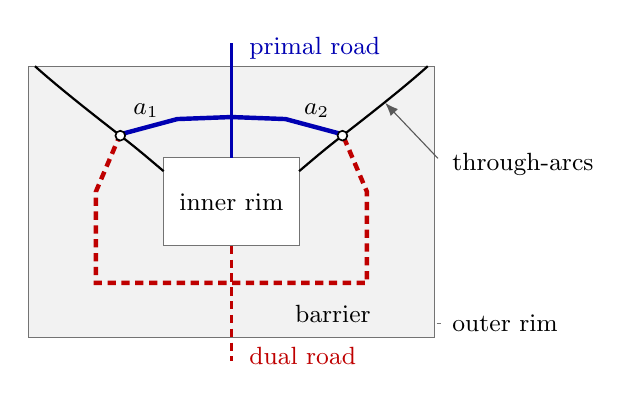
\begin{tikzpicture}[x=0.86cm,y=0.86cm,>=Latex,
  every node/.style={font=\small}]
  \fill[black!5] (-3,-2) rectangle (3,2);
  \fill[white] (-1,-.65) rectangle (1,.65);
  \draw[black!55] (-3,-2) rectangle (3,2);
  \draw[black!55] (-1,-.65) rectangle (1,.65);
  \node at (0,0) {inner rim};
  \node[anchor=west] at (3.12,-1.8) {outer rim};
  \draw[black!55] (3.03,-1.8)--(3.1,-1.8);

  \draw[blue!70!black,line width=1.35pt]
    (0,.65)--(0,2.35);
  \draw[red!75!black,line width=1.35pt,densely dashed]
    (0,-.65)--(0,-2.35);
  \node[anchor=west,text=blue!70!black] at (.12,2.27)
    {primal road};
  \node[anchor=west,text=red!75!black] at (.12,-2.27)
    {dual road};

  \draw[blue!70!black,line width=1.6pt]
    (-1.62,1.00)--(-.8,1.22)--(0,1.25)--(.8,1.22)--(1.62,1.00);
  \draw[red!75!black,line width=1.6pt,densely dashed]
    (1.66,.95)--(2,.15)--(2,-1.2)--(-2,-1.2)--(-2,.15)--(-1.66,.95);
  \draw[black,line width=1.1pt] (1.62,1.00)--(1.66,.95);
  \draw[black,line width=1.1pt] (-1.62,1.00)--(-1.66,.95);

  \draw[black,line width=.8pt]
    (1,.45).. controls (1.26,.67) and (1.40,.79) .. (1.64,.975)
      .. controls (1.98,1.24) and (2.52,1.66) .. (2.9,2);
  \draw[black,line width=.8pt]
    (-1,.45).. controls (-1.26,.67) and (-1.40,.79) .. (-1.64,.975)
      .. controls (-1.98,1.24) and (-2.52,1.66) .. (-2.9,2);
  \draw[black,fill=white,line width=.6pt] (1.64,.975) circle (.072);
  \draw[black,fill=white,line width=.6pt] (-1.64,.975) circle (.072);
  \node[anchor=south east] at (1.59,1.10) {$a_2$};
  \node[anchor=south west] at (-1.59,1.10) {$a_1$};
  \node[anchor=west] at (3.12,.55) {through-arcs};
  \draw[black!65,->] (3.05,.64)--(2.27,1.46);
  \node at (1.5,-1.65) {barrier};
\end{tikzpicture}

\caption{The topological consequence of the reference-band
construction.  A primal path and a dual path form a route of winding
number one around the inner rim, with exactly two adjacency steps
$a_1,a_2$ between colors.  Only those steps can cross medial strands.
Hence at most two strand arcs can cross the band; the two radial
color roads force both to be present.  The picture is schematic:
the adjacency steps are enlarged, the flanking crossings used to
construct the route are omitted, and neither the color paths nor
the medial arcs are asserted to be straight or smooth.}
\label{fig:barrier}
\end{figure}

\subsection{Landing extensions and gluing}

We use a strengthened form of arm separation which retains the
crossing clusters.  For a fixed-ratio bulk annulus and every
$\varepsilon>0$, the probability in the plane FK law that some crossing arms admit no
separated landing extensions in their respective original color
clusters is at most $\varepsilon$, when the separation parameter is
chosen small enough.  This is precisely the event $B_n$ preceding
Lemma~5.9 of \cite{CDCH}.  The replacement arms there are required to
belong to the same respective primal or dual clusters.  The proof
uses the quadrilateral crossing bounds, including at the exposed
jagged sides, the small- and large-extremal-length bounds, and an
upper bound on the number of crossing components.  These are all
available for $1\le q<4$ by \cite[Theorem~1.2 and Section~6]{DMT};
indeed its proof of Proposition~6.2 invokes this argument.  Thus we
use the proof at its stated probabilistic inputs, rather than an
Ising-specific identity.

We need two geometric features of these extensions.  Their endpoints
stay away from the corners of the square cut, and the extension
boxes can be much smaller than the separation between different
landings.  In the proof of \cite[Lemma~5.9]{CDCH}, separation occurs
at the scale denoted there by $\delta^3 n$, whereas extensions are
constructed at smaller scales $\delta^k n$, $k\ge4$.  Only finitely
many such scales are needed for a specified error tolerance.  The
arms consequently protrude a positive relative distance beyond
their landing cut, inside disjoint boxes having a fixed-factor
margin between them.  All constants may depend on the error
tolerance.  Bounded lattice rounding is harmless once the trial
scale exceeds a corresponding fixed minimum.

Suppose a past has been exposed up to a square cut of radius $l$,
and the conditional, unconditioned-FK probability that the specified
start reaches a larger cut of radius $8l$ is at least $h>0$.
Here and below the factors $8$ and $16$ may be increased by fixed
amounts to accommodate collars.  Apply the preceding landing
statement on an annulus strictly between those two cuts.  Its
failure event can be assigned ordinary plane probability less than
$h/(2C)$, where $C$ is the collar-comparison constant.  Its
conditional probability given the past is then less than $h/2$.
Thus, with conditional probability at least $h/2$, the two
start-connected clusters have separated outer extensions before
radius $16l$.  The crossing portions are taken after their last
visits to the annulus's inner rim.  Replacing those portions within
their same clusters preserves connection to the start.  A finite
cover of the landing rim by small boxes allows the landing
locations to be restricted to one pair of boxes, at a cost depending
on $h$ only.

There is a corresponding construction facing inward from the
remaining annulus toward $R$.  Arms beginning at a scale comparable
to $K l$, where $K$ is a sufficiently large fixed number, can have
separated inward protrusions and can be required to reach a little
beyond the target cut.  Their probability is bounded below by
$c\pi_2(l,R)$.  To check the relative cost of the landing failure,
crop the remaining arms through a fixed-ratio buffer before the
annulus where the landing test is performed.  Collar comparison
and quasimultiplicativity bound the joint probability of that
failure and the remaining arms by
$C\varepsilon\pi_2(l,R)$.  Choose $\varepsilon$ small, or use the
equivalent well-separated-arm comparison.  This also shows that
the construction is uniform under conditioning on data separated
from it by the specified collars.

The two sets of protrusions can be joined through the free space
between them.  Group their locations on a sufficiently fine but
fixed grid along each cut.  For every resulting pair of location
choices, there are disjoint corridors joining the primal tabs and
the dual tabs, with widths bounded below by a positive multiple
of $l$.  The constants can be small functions of $h$; they do not
change the total number of geometric trial scales.  In a
protrusion box, require a transverse crossing at a level between
the landing cut and the protrusion's outermost required level.
It must meet the protruding arm.  Overlapping longitudinal and
transverse crossings then carry that contact through its corridor.
Only one color is involved in each corridor and its overlap boxes.
The conditional crossing estimates and FKG in that color give a
positive fixed gluing probability.  This is the tube construction
of \cite[Proof of Proposition~5.4]{CDCH}.

The distinction between the central band and its extensions is
essential here.  An arbitrary event $E$ may fix \emph{every edge}
of the central band, so no gluing edge is allowed to lie there.
The protrusions extend outside that band; their overlap boxes and
the connecting corridors lie strictly outside it.  Within an
overlap box the only requirement inherited from the extension is
a connection in that box's color, which is increasing in its
color edges.  Thus FKG applies after $E$ is fixed.  The auxiliary
extensions are integrated out when we take a measure on the
central-band configurations.  They are not additional band data
that must agree in the eventual coupling.

\subsection{Frequent opportunities under the conditioned law}

We now prove Proposition~\ref{prop:outward}.  Denote the common
ambient law, including its permitted exterior reweighting, by
$\Pp_0$, and write
\[
 Q_a=\Pp_0(\,\cdot\mid S_R(a))
\]
for a particular start $a$.  Until the target scale, all conditional
edge laws before the $S_R(a)$ conditioning are ordinary FK laws
with induced partitions, or mixtures of such laws.  Consequently
the collar and crossing comparisons just established apply to
$\Pp_0$ as well.

Choose a fixed large ratio $K$ leaving room for the past-extension
annulus, the reference band with its two collars, and the
outer-extension annulus.  Trial radii are
$l_i=K^i l_0$, where $l_0$ is a fixed large multiple of $s$,
increased to a fixed minimum mesh scale when necessary.  Stop the
trials before a fixed fraction of $R$.  The number $k$ of available
trials satisfies
\[
 k\ge \frac{\log(R/s)}{\log K}-C.
\]
When the right side is bounded, enlarging the constant in
\eqref{eq:outward-error} suffices.  We may therefore assume there
are many trials.

Let $\mathcal F_i$ contain all edges inside the radius-$l_i$ cut,
together with the identities of the start-connected color
regions there.  Call trial $i$ good for start $a$ if
\begin{equation}\label{eq:good-trial}
 \Pp_0(S_{8l_i}(a)\mid\mathcal F_i)\ge h.
\end{equation}
The threshold $h>0$ is chosen after $K$.  The preceding separation
and gluing constructions then use narrower corridors if necessary;
they require no increase of $K$ depending on $h$.

Under $Q_a$, with probability at least $1-Ce^{-c k}$, at least
$3k/4$ of the trials are good.  Here is the conditioning calculation.
The event $S_R(a)$ implies $S_{8l_i}(a)$ at every trial.  For a
specified collection $J$ of bad trials, expose success to
$8l_i$ before passing to the next selected trial.  Since badness is
$\mathcal F_i$-measurable, the tower property and the negation of
\eqref{eq:good-trial} give a factor at most $h$ for each $i\in J$.
Moreover, by \eqref{eq:start-probabilities} and
quasimultiplicativity,
\[
 \frac{\Pp_0(S_R(a))}{\Pp_0(S_{l_0}(a))}
       \ge C^{-1}e^{-C_0 k}.
\]
The microscopic or one-arm factors in
\eqref{eq:start-probabilities} cancel in this ratio.  Summing over
collections of at least $k/4$ bad trials gives
\begin{equation}\label{eq:good-trial-tail}
 Q_a\{\text{at least }k/4\text{ bad trials}\}
 \le C e^{C_0 k}2^k h^{k/4}.
\end{equation}
Choose $h$ so small that the right side decreases exponentially
in $k$.  This choice is uniform over all the permitted starts and
exterior laws.

\subsection{A common band measure and loss of the past}

At a good trial, place a scaled copy of the reference band between
the past-extension and outer-extension annuli.  Its central
configuration has a subprobability measure $\nu_l$ defined as
follows: take the plane FK law, restrict to the successful
reference-band construction of Lemma~\ref{lem:reference-band},
including the auxiliary protrusions, and then retain only the
central-band edges.  There is a fixed $v_0>0$ such that
$\nu_l(\text{all band data})\ge v_0$.

For every event $E$ of central-band data and every good past,
\begin{equation}\label{eq:band-minorization-raw}
 \Pp_0\{\text{band data}\in E,\ S_R(a)
                     \mid\mathcal F_i\}
       \ge c_h\,\nu_l(E)\,\pi_2(l,R).
\end{equation}
Indeed, the good past supplies the separated start-connected
extensions with probability bounded below in terms of $h$.
Require the reference-band event with its protrusions, and
separated arms continuing toward $R$.  Before gluing, these
observations are separated by full collars.  Bounded-density
comparison can therefore be applied successively from the two
sides of the central band.  It preserves the factor $\nu_l(E)$
for an arbitrary, possibly nonmonotone, set $E$, and gives the
factor $\pi_2(l,R)$ for the remaining arms.  There is still
unobserved space for the two-color tube construction.  Its
same-color overlap requirements leave $E$ fixed, as explained
above, and complete both paths from the start to the target.
This proves \eqref{eq:band-minorization-raw}.

To make the averaging explicit, condition beyond a collar
containing all these constructions, and let $\xi$ denote the
resulting exterior state.  Given the already fixed past, write
$p_\xi$ for the conditional probability of reaching $8l$ and
$\mu$ for the conditional distribution of $\xi$.  Goodness
means $\int p_\xi\,\mu(\dd\xi)\ge h$; it does not assert
$p_\xi\ge h$ for each $\xi$.  Uniform collar comparison makes
the landing-error probability at most $\varepsilon$ for every
$\xi$, with $\varepsilon<h/2$.  In the preceding construction,
keep the probability of the start-connected extensions as a
factor instead of replacing it by a constant.  The finitely
many landing-location choices all have the same lower gluing
bound.  The conditional lower bound is therefore
\[
 c\nu_l(E)\pi_2(l,R)(p_\xi-\varepsilon)_+.
\]
Its integral is at least
$c\nu_l(E)\pi_2(l,R)(h-\varepsilon)$, as required in
\eqref{eq:band-minorization-raw}.  This proves the assertion for
the exterior mixture without imposing pointwise goodness.
No identification jumps an annulus used in these comparisons.

In the reverse direction, any successful continuation from the
past must have two arms in the remaining annulus.  Cropping
through a collar and using \eqref{eq:start-probabilities} gives
\begin{equation}\label{eq:band-denominator}
 \Pp_0(S_R(a)\mid\mathcal F_i)\le C\pi_2(l,R).
\end{equation}
Dividing \eqref{eq:band-minorization-raw} by
\eqref{eq:band-denominator} shows that, under $Q_a$, the band
marginal after every good past dominates $c\nu_l$.  Hence two
good pasts, even for different starts, have a uniformly positive
common part on identical central-band data.

It remains to check that coupling this band is enough.  Cut its
strands at both rims.  There are two through-arcs.  All remaining
arcs have both ends on the same rim.  Whatever the configuration
inside the inner rim, completing its pairings joins the two
through-arcs to one another: they are the only two strand ends
left after the same-rim arcs and the interior pairings are
followed.  Interior loops can change in number, but their loop
weight is then a factor depending solely on that interior
completion.  The effective pairing seen on the outer rim is
fixed by the band.

The same fact can be expressed in FK terms.  Exactly one primal
region and one dual region transmit through the band.  An
exterior connection that enters the past must do so through the
transmitted region of its color, whose trace on the outer rim is
already determined by the band.  Thus the induced exterior
primal partition is independent of the earlier past.  On $S_R(a)$,
the starting regions have made contact with these two transmitted
regions.  Conditional on that contact, the remaining constraint
is only that the transmitted regions continue to the target
cut.  Paths that cross the band repeatedly use the same
transmitted region and impose no additional constraint.  The
domain Markov property now shows that the conditional law on
and outside the outer rim, given the common band and successful
continuation, is identical for the two pasts.  A common exterior
weight or an ambient wall farther out changes this common law
in the same way in both cases.

We can therefore complete the coupling as follows.  At each trial,
if both pasts are good, use the common submeasure $c\nu_l$ to
couple the central-band configurations with probability at least
$p>0$.  On success, fill the interior gaps according to their
respective conditional laws and sample the exterior from the
common conditional law just described.  On failure, use the
residual band marginals and fill the data up to the next trial
cut with their correct conditional laws.  No edges beyond that
next cut are inspected merely to decide whether a coupling
attempt failed.  This is a coupling of the successive conditional
kernels, so each complete marginal remains $Q_a$ throughout.

For completeness, this iteration does not require the trials to
be independent.  By \eqref{eq:good-trial-tail} and a union bound
over the two marginals, except with probability $Ce^{-c k}$
there are at least $k/2$ jointly good trials.  Their goodness is
known from the two pasts before the corresponding attempt.
At each such trial, conditional on the entire coupled past and
on all earlier failures, the overlap probability is at least
$p$.  Iterating at these predictable trial times bounds the
probability of $k/2$ failed good attempts by $(1-p)^{k/2}$.
The total failure probability is consequently at most
$Ce^{-c'k}\le C(s/R)^c$.  On success the band and its exterior
agree, and the two transmitted color regions have been reached
by both starts.  This proves Proposition~\ref{prop:outward}.

For a tile-side start, the common through-strand passes through
the associated medial segment: otherwise that segment would lie
on a completed inner loop surrounding one of its two end sites,
contrary to $S_R(e)$.  For a disk start, the common through-strand
meets the disk, since every disk-to-target strand must pass
through the band.  Thus an exterior rule selecting the
distinguished Dobrushin strand gives the same verdict for a
microscopic segment and for a disk after successful coupling.
This is the form used in the occupation comparison.

\section{From electric correlations to microscopic normalization}
\label{sec:calibration}

The electric formula is accurate when marked points remain separated
by a mesoscopic distance. Counting an edge requires two opposite-color
marked points at distance one. The outward coupling bridges these
scales. We first obtain a pure-power amplitude for a neighboring pair,
then compare that pair with a disk. The latter comparison is the
normalization needed for occupation measures.

\subsection{A signed factor with positive local conditioning}

Fix the two neutral charge groups of
Proposition~\ref{prop:special-charges}. Each group has a core charge
$\alpha=\pi/2-\lambda$ and sufficiently many small negative
compensating charges. Place the compensators at distinct points
$u_j(n)$ on the axis by fixed, color-preserving lattice roundings
$u_j(n)=n\zeta_j+O(1)$, where the $\zeta_j$ are distinct fixed
locations away from the origin. The two cores lie within distance
$r=o(n)$ of the origin, in opposite colors. The first core is held
fixed. Write $e$ for the neighboring pair corresponding to a medial
segment, and write $r$ for the separated pair, with the appropriate
odd lattice separation. All rounding conventions preserve these
colors.

Let
\[
 B_* = \sum_{j\text{ remote}}\beta(t_j),\qquad
 \beta(t)=-A(t^2+2\lambda t),\qquad
 A=\frac{1}{2\pi(\pi-\lambda)}.
\]
Choose disjoint small patches of radius a fixed multiple of $n$ around
the remote points. Reweight only the loops wholly contained in these
patches, using their single-point weights
$v(t_j)=\cos(\lambda+t_j)/\cos\lambda$. These weights are positive.
Let $Z_*(n)$ be the mass of this local reweighting and let
$\Pp_n^*$ be its normalized probability law. The cutoff comparison
and the pure-nest asymptotic give
\begin{equation}\label{eq:proxy-mass}
 Z_*(n)\asymp\prod_{j\text{ remote}}F_n(v(t_j))
 \asymp n^{B_*}.
\end{equation}
Constants are uniform over the finitely many rounding classes used
below. We use the positive-winding expansion of the electric
correlation. Its remaining loop factor, denoted by $Y_r$, need not
be nonnegative.

Let $R$ be larger than the core separation by a fixed factor and
smaller than a sufficiently small multiple of $n$. The event $S_R(r)$
means that both core colors reach the tile rim of radius $R$.
The scalar weight of a loop enclosing just one core and no remote point
is zero, because $\cos(\lambda+\alpha)=0$. A completed loop inside
the $R$-disk enclosing both opposite-color cores contains another
loop separating them. Thus any nonzero configuration has $S_R(r)$.
Conversely, factoring out its indicator merely restricts the original
loop product. Consequently the full electric correlation satisfies
\begin{equation}\label{eq:core-factorization}
 C_r(n)=Z_*(n)\Pp_n^*(S_R(r))
             \E_n^*[Y_r\mid S_R(r)].
\end{equation}
The same identity holds for the neighboring pair $e$.

We record two uniform bounds used throughout this section. For every
fixed $j\ge1$,
\begin{align}
 \E_n^*[|Y_r|^j\mid S_R(r)]&\le C_j,
 \label{eq:macro-moments}\\
 \frac{\Pp_n^*(S_R(r))}{\Pp(S_R(r))}
 &=1+O((R/n)^{c_0}).
 \label{eq:proxy-local-probability}
\end{align}
Here $\Pp$ denotes the ordinary plane FK law; the same statements hold
with $r$ replaced by $e$. To justify the first bound, discard
configurations on which $Y_r=0$. Every non-unit factor remaining
on the other configurations belongs to a macroscopic loop.
A separating loop must enclose a remote point, and an ancestor
enclosing both cores contains such a separating loop. A loop charged
only at remote points but not included in the local reweighting has
left its remote patch. Each such loop therefore has a passage through
one of finitely many buffered regions of size comparable to $n$.
These buffers may be chosen away from the support of $S_R(r)$.
Even a loop with an arbitrarily large excursion has such a passage.
Conditional passage moments and the local-tilt estimate of
Input~\ref{inp:fk} control every fixed moment of the product.
Cutting the arm event back by a fixed factor leaves collars before
the passage buffers, so the estimates cost its ordinary probability,
not its reciprocal. This gives \eqref{eq:macro-moments} after
normalization. The relative collar comparison gives
\eqref{eq:proxy-local-probability}, because the nonnegative local
reweighting is supported at distance comparable to $n$.

\begin{lemma}\label{lem:signed-comparison}
Consider two opposite-color core pairs contained in a disk of radius
$s$, with the same remote charges and local reweighting. If
$Cs<R<cn$, then
\[
 \left|\E_n^*[Y_1\mid S_R(1)]-
             \E_n^*[Y_2\mid S_R(2)]\right|
 \le C(s/R)^{c_1}.
\]
The constants are independent of the microscopic separations of the
pairs.
\end{lemma}

\begin{proof}
Apply Proposition~\ref{prop:outward} to the two starts, with the common
nonnegative remote reweighting. On successful coupling the band and
the entire exterior agree. Exactly one global loop has the two
through-arcs in that band. It separates the opposite-color cores:
an inner closure separating them would contradict $S_R$. Its
enclosures of remote points are the same in both configurations.
Every other loop outside the band either encloses both cores or
neither, and the ancestors of the through-loop enclose both.
Inside the band no completed loop can enclose a core under $S_R$.
The factors $Y_1,Y_2$ therefore agree on successful coupling.
H\"older's inequality and \eqref{eq:macro-moments} bound their
contribution on coupling failure by a positive power of its probability.
Reducing the exponent in Proposition~\ref{prop:outward} proves the
claim. No positivity of $Y_i$ is used.
\end{proof}

\subsection{The neighboring-pair amplitude}

Set $x_1=-\beta(\alpha)$. The parameter identities are
\begin{equation}\label{eq:exponent-identity}
 2x_1+2A\alpha^2=x,
 \qquad
 x=\frac{\pi-2\lambda}{2(\pi-\lambda)}.
\end{equation}
For a sufficiently small fixed $\xi>0$, choose an odd separation
$r\asymp n^{1-\xi}$. Proposition~\ref{prop:special-charges} gives
\begin{equation}\label{eq:mesoscopic-core}
 \begin{split}
 C_r(n)
 &=M_* n^{B_*-x}r^{2A\alpha^2}(1+O(n^{-c_2}))\\
 &=M_* n^{B_*}r^{-2x_1}(r/n)^x(1+O(n^{-c_2})),
 \qquad M_*\ne0.
 \end{split}
\end{equation}
The amplitude depends on the fixed remote geometry, charges, and
rounding convention, but not on $n$ or $r$ in this regime. Indeed the
full Coulomb formula uses the actual pairwise distances; replacing
the remote distances from either core by their limiting values changes
its product by $O(r/n)+O(n^{-1})$. These errors can be included in
the power remainder. We will not use this equivalence with a fixed
$M_*$ when $r/n$ is held positive.

\begin{proposition}\label{prop:microscopic-amplitude}
For the fixed remote experiment there exists $c_*\ne0$ such that
\begin{equation}\label{eq:microscopic-amplitude}
 C_e(n)=c_*n^{B_*-x}(1+O(n^{-c_3})).
\end{equation}
In particular this limit holds through all positive integers $n$.
\end{proposition}

\begin{proof}
Take
\[
 r\asymp n^{1-\xi},\qquad R\asymp n^{1-b\xi},
 \qquad 0<b<1.
\]
All radii are chosen once for the comparison interval $[n,2n]$.
From \eqref{eq:core-factorization}, \eqref{eq:proxy-mass},
\eqref{eq:mesoscopic-core}, the one-arm bound, and
\eqref{eq:start-probabilities}, we obtain, for every small
$\delta>0$,
\begin{equation}\label{eq:expectation-lower}
 \left|\E_n^*[Y_r\mid S_R(r)]\right|
 \ge c_\delta(R/n)^x(r/R)^\delta.
\end{equation}
For example the upper estimate
$\Pp(S_R(r))\le C_\delta r^{-2x_1}(r/R)^{x-\delta}$
in the denominator gives precisely this inequality.
Its right side has order
$n^{-[bx+\delta(1-b)]\xi}$, whereas the signed comparison error
is $O(n^{-c_1(1-b)\xi})$. Choose $b>0$ sufficiently small and then
$\delta>0$ sufficiently small that
\[
 c_1(1-b)>bx+\delta(1-b).
\]
Lemma~\ref{lem:signed-comparison} is then a relative power-error
comparison of the two conditional expectations.

Apply the same argument with the remote geometry at any integer scale
$N\in[n,2n]$, using the \emph{same} core positions, $r$, and $R$.
Equation~\eqref{eq:proxy-local-probability} removes the remote tilt
from the arm probabilities with a power error. Uniformly in this
interval,
\begin{equation}\label{eq:fixed-radii-ratio}
 \frac{C_e(N)}{C_r(N)}
 =\frac{\Pp(S_R(e))}{\Pp(S_R(r))}(1+O(n^{-c_4})).
\end{equation}
The ordinary probability ratio on the right does not depend on $N$.
The mesoscopic formula therefore yields
\begin{equation}\label{eq:dyadic-amplitude-ratio}
 \frac{N^{x-B_*}C_e(N)}{n^{x-B_*}C_e(n)}
 =1+O(n^{-c_5}),\qquad n\le N\le2n.
\end{equation}
The denominator is nonzero for all sufficiently large $n$, since
\eqref{eq:expectation-lower} dominates the coupling error.

Write $a_n=n^{x-B_*}C_e(n)$. On a dyadic sequence, the consecutive
ratios of $a_n$ differ from one by a summable sequence. Their product
converges to a nonzero value, with tail error $O(n^{-c_5})$.
Equation~\eqref{eq:dyadic-amplitude-ratio} compares every intervening
integer to the preceding dyadic scale. Hence the entire sequence has
the same nonzero limit and the stated power error.
\end{proof}

\begin{proposition}\label{prop:sharp-arms}
For all radii above a fixed lattice scale,
\begin{equation}\label{eq:sharp-arms}
 \Pp(S_R(e))\asymp R^{-x},\qquad
 \pi_2(r,R)\asymp(r/R)^x.
\end{equation}
The estimates hold with fixed-factor changes of the inner and outer
rims and with a further bulk collar.
\end{proposition}

\begin{proof}
First choose $R=\theta n$, with $\theta>0$ a sufficiently small fixed
constant. Equations~\eqref{eq:core-factorization},
\eqref{eq:macro-moments}, and~\eqref{eq:microscopic-amplitude}
give the lower bound $\Pp(S_R(e))\ge c n^{-x}$.

For the reverse bound, compare the neighboring pair with an
opposite-color pair at separation $r\asymp aR$, where $a>0$ is a
small fixed constant. Use the full Coulomb formula, not the
$r=o(n)$ simplification with its limiting amplitude. Its magnitude
is uniformly comparable to
$n^{B_*}r^{-2x_1}(r/n)^x$ as first $n\to\infty$ and then
$a\downarrow0$. The nonzero amplitude and the remote-distance
factors vary continuously in this limit. It follows that
\[
 \left|\E_n^*[Y_r\mid S_R(r)]\right|
 \ge c_\delta\theta^x a^\delta.
\]
Choose $\delta<c_1$ and then $a$ small enough that
$Ca^{c_1}<\tfrac12 c_\delta\theta^x a^\delta$.
Lemma~\ref{lem:signed-comparison} gives a strictly positive lower
bound for the magnitude of the conditional expectation at $e$.
Equation~\eqref{eq:core-factorization} now gives
$\Pp(S_R(e))\le C n^{-x}$. Fixed-factor extensions cover all large
$R$, and finite energy covers the remaining bounded scales.

The first line of \eqref{eq:start-probabilities} identifies
$\Pp(S_R(e))$ with $\pi_2(C,R)$. Quasimultiplicativity therefore gives
\[
 \pi_2(r,R)\asymp
 \frac{\pi_2(C,R)}{\pi_2(C,r)}\asymp(r/R)^x.
\]
All comparisons used buffered events, so their collar and rounding
versions follow from the same fixed-factor estimates.
\end{proof}

\subsection{Calibration by disk probes}

A disk does not carry a prescribed electric charge. We therefore
introduce a diagnostic loop factor which agrees with the neighboring
pair's factor after successful outward coupling. Its purpose is only
to determine deterministic normalization constants.

Let $s=\epsilon n<R$. Under the same remote local reweighting, let
$S_R(s)$ be the disk two-arm event. If exactly one global loop touches
the disk and leaves the $R$-cut, assign that loop the factor it would
receive as a separator of the two cores, with its actual remote
enclosures. Give its ancestors the factors corresponding to enclosing
both cores, and give other loops no core charge. Divide out the local
remote weights already included in $\Pp_n^*$. Call the resulting
factor $Y_s$. In every other case set $Y_s=0$. In particular the
distinguished loop receives value zero when it encloses no remote
point. Define the deterministic quantity
\begin{equation}\label{eq:disk-diagnostic}
 W_s(n)=Z_*(n)\Pp_n^*(S_R(s))
                       \E_n^*[Y_s\mid S_R(s)].
\end{equation}
The moment bound \eqref{eq:macro-moments} also holds for $Y_s$:
every charged loop in a nonzero configuration spans between the disk
and a remote patch, or leaves a remote patch.

In the coupling of the disk start and the edge start, the factors
$Y_s$ and $Y_e$ coincide on success. The unique band through-loop
touches the disk, and no second loop can both touch the disk and leave
$R$. Replacing its inside portion preserves its remote enclosures;
the same is true for its ancestors. Thus
\begin{equation}\label{eq:disk-signed-comparison}
 \left|\E_n^*[Y_s\mid S_R(s)]-
             \E_n^*[Y_e\mid S_R(e)]\right|
 \le C(s/R)^{c_6}.
\end{equation}

\begin{lemma}\label{lem:disk-diagnostic}
For almost every fixed pair of scaled radii $0<\epsilon<\theta$
in the permissible range, with $s=\epsilon n$ and $R=\theta n$,
the limit
\begin{equation}\label{eq:diagnostic-limit}
 \lim_{n\to\infty}n^{-B_*}W_s(n)
\end{equation}
exists. Tile-rim roundings do not change the limit.
\end{lemma}

\begin{proof}
We use Corollary~\ref{cor:macroscopic-test}. First remove the nest weights
below radius $\delta n$ at each remote point, dividing by the
corresponding single-point nest partition functions. Their inward
coupling and cutoff insensitivity make the normalized error tend to
zero as $\delta\downarrow0$, uniformly in $n$.

There is a minor extra condition here: a loop deciding the disk
diagnostic might enter one of those small neighborhoods. It can be
discarded at a vanishing cost. Indeed the positive remote tilt produces
a surrounding screen before reaching the neighborhood with probability
tending to one. A loop arriving from the distant disk cannot cross
that screen. More annular trials reduce the exceptional probability,
and the moment bound for the remaining loop factors makes its weighted
contribution vanish. Thus, outside a vanishing exceptional event, the
diagnostic is determined by the truncated macroscopic configuration.

For fixed $\delta$, truncate excursions beyond a large fixed multiple
of $n$ and the number of charged macroscopic passages. The remaining
test uses finitely many loops of diameter bounded below after scaling.
It reads their ordered trajectories, their windings about the remote
points, and their intersections with the two disk rims. In a nonzero
diagnostic, ancestors of the distinguished loop can be recognized
among the remote-enclosing loops by whether they enclose the disk
center: any other such loop is disjoint from the disk, since otherwise
it too would touch the disk and leave $R$.

Input~\ref{inp:loops} gives convergence of these loop tests. Fixed
marked points are almost surely off all macroscopic loop traces.
For almost every choice of radii, no relevant loop is at a tangency
threshold, so intersection tests are continuity events. This follows
also by Fubini from the countable loop collection and its matching
topology. Bounded tile-rounding errors do not affect such tests.
The passage moment bounds remove the count and excursion truncations.
Finally let $\delta\downarrow0$. The pure-power asymptotics of the
remote nest factors identify their normalization with $n^{B_*}$,
proving \eqref{eq:diagnostic-limit}.
\end{proof}

\begin{proposition}\label{prop:disk-calibration}
There is a sequence $\epsilon\downarrow0$, a choice of radii
$R/n\asymp\epsilon^b$, and positive deterministic numbers
$L_\epsilon\asymp\epsilon^{-x}$ such that
\begin{equation}\label{eq:disk-calibration}
 \limsup_{n\to\infty}
 \left|
 \frac{n^x\Pp(S_R(e))}{L_\epsilon\Pp(S_R(\epsilon n))}-1
 \right|\le C\epsilon^{c_7}.
\end{equation}
The exponent $b>0$ may be chosen sufficiently small in advance to
satisfy any additional finitely many inequalities of the form
$(1-b)c>bx$, with $c>0$ fixed. The same constants apply to every
translate and rotation of the edge start, including color exchange.
\end{proposition}

\begin{proof}
Write $t=R/n$. Equations~\eqref{eq:core-factorization},
\eqref{eq:proxy-mass}, \eqref{eq:microscopic-amplitude}, and
\eqref{eq:sharp-arms} imply
\begin{equation}\label{eq:edge-expectation-size}
 \left|\E_n^*[Y_e\mid S_R(e)]\right|\asymp t^x.
\end{equation}
For $t\asymp\epsilon^b$, the relative error in
\eqref{eq:disk-signed-comparison} is bounded by
$C\epsilon^{(1-b)c_6-bx}$. Choose $b$ so that this exponent is
positive; it can simultaneously satisfy the stated finite collection
of further inequalities. The relative collar error in
\eqref{eq:proxy-local-probability} is $O(\epsilon^{bc_0})$.
Consequently
\begin{equation}\label{eq:disk-ratio-identity}
 \frac{n^x C_e(n)}{W_s(n)}
 =\frac{n^x\Pp(S_R(e))}{\Pp(S_R(s))}
                    (1+O(\epsilon^{c_7}))
\end{equation}
for a positive exponent $c_7$ after it is decreased if necessary.
Although the two correlations can be signed, their ratio in this
display is positive for small $\epsilon$, by the relative comparison.

Choose a sequence of continuity pairs for
Lemma~\ref{lem:disk-diagnostic}, with
$R/n\asymp\epsilon^b$. The sharp arm estimates show that the right
side of \eqref{eq:disk-ratio-identity} is comparable to
$\epsilon^{-x}$. Thus the limit of $n^{-B_*}W_s(n)$ is nonzero for
each sufficiently small chosen $\epsilon$. Define
\[
 L_\epsilon=
 \frac{c_*}{\displaystyle\lim_{n\to\infty}n^{-B_*}W_s(n)}.
\]
The numerator is the amplitude in
\eqref{eq:microscopic-amplitude}. This definition and
\eqref{eq:disk-ratio-identity} give positivity,
$L_\epsilon\asymp\epsilon^{-x}$, and
\eqref{eq:disk-calibration}.

All probabilities in \eqref{eq:disk-calibration} are ordinary plane
probabilities. Translation, square symmetries, and planar self-duality
identify them for the different edge locations and orientations, using
covariant tile-disk roundings. Therefore the calibration does not
depend on the checkerboard class or orientation of the probe.
\end{proof}

\section{Occupation measures and the whole trace}
\label{sec:occupation}

Proposition~\ref{prop:disk-calibration} compares a microscopic segment
with a disk whose radius is a fixed fraction of the domain size.  We
first make this comparison inside second moments.  The resulting
approximation permits us to use ordered-curve convergence at a fixed
disk radius, and only afterwards let that radius tend to zero.  We
also control the boundary strip, since weak convergence of finite
measures on the closed square includes convergence of total mass.

\subsection{Segment probes and their replacement by disks}

Let $\mathcal E_n$ be the deterministic set of full medial segments
available in the discrete square, including the boundary collar of
Section~\ref{sec:introduction}.  A segment here is an edge of the drawn
medial graph, before applying $\Pi$.  Write $z_e$ for its projected
midpoint and $I_e$ for the indicator that it belongs to the distinguished
strand.  The pairing at every medial vertex splits that vertex into
two vertices of degree two.  In the resulting finite graph, the
component containing a distinguished terminal half-edge is a path,
with the other distinguished half-edge as its other end.  It cannot
repeat an edge: a repeated edge would put that component on a cycle,
which cannot contain its degree-one terminal vertices.  Consequently
the counting multiplicity in~\eqref{eq:counting-measure} is exactly
$I_e$, even when the unsplit medial vertex is visited twice.  Distinct
collar edges are still counted separately if their projections coincide.

There is a constant $A_0>0$, determined by the density of medial
midpoints in the stated lattice units, such that
\begin{equation}
 A_0n^{-2}\sum_{e\in\mathcal E_n}h(z_e)
 \longrightarrow \int_D h(z)\dd A(z)
 \qquad\bigl(h\in C(\overline D)\bigr).
 \label{eq:probe-riemann}
\end{equation}
Indeed the bulk midpoints form a periodic set of fixed density, and
there are only $O(n)$ additional boundary probes.  Define
\begin{equation}
 X_n(f)=A_0n^{-2}\sum_{e\in\mathcal E_n}f(z_e)n^x I_e
       =A_0n^{-d}\sum_{e\in\mathcal E_n}f(z_e)I_e.
 \label{eq:microscopic-test}
\end{equation}

Use the sequence of radii $\epsilon\downarrow0$ supplied by
Proposition~\ref{prop:disk-calibration}, together with its constants
$L_\epsilon\asymp\epsilon^{-x}$.  The physical scale of a unit tile is
$a_0/n$.  For a probe $e$ in the bulk, let $B_e^\epsilon$ be the
whole-tile disk of radius $s=\epsilon n$ used in that proposition,
translated to the probe.  Its physical radius is $a_0\epsilon$, up to
$O(n^{-1})$.  Let $J_e^\epsilon$ indicate that the distinguished strand
enters this disk; the occurrence of an unrelated loop does not count.
For $f\in C_c(D)$, put
\begin{equation}
 X_{n,\epsilon}(f)
   =A_0n^{-2}\sum_{e\in\mathcal E_n}f(z_e)L_\epsilon J_e^\epsilon.
 \label{eq:disk-test}
\end{equation}
For fixed $\epsilon$ sufficiently small, every disk occurring in this
sum is inside $D$ once $n$ is sufficiently large.

\begin{proposition}[Replacement in second moment]
\label{prop:l2-replacement}
For every real $f\in C_c(D)$,
\begin{equation}
 \lim_{\epsilon\downarrow0}\limsup_{n\to\infty}
 \E\bigl[|X_n(f)-X_{n,\epsilon}(f)|^2\bigr]=0,
 \label{eq:l2-replacement}
\end{equation}
where $\epsilon$ tends to zero through the sequence in
Proposition~\ref{prop:disk-calibration}.  The same approximation holds
for every finite vector of such tests.
\end{proposition}

\begin{proof}
Fix a compact set $K\Subset D$ containing $\supp f$, and abbreviate
\[
 H_e^0=I_e,\qquad H_e^1=J_e^\epsilon,
 \qquad w_0=n^x,\qquad w_1=L_\epsilon,
 \qquad V_e^a=w_aH_e^a\quad(a\in\{0,1\}).
\]
We first compare products at two probes $e,e'$ satisfying
$z_e,z_{e'}\in K$ and $|z_e-z_{e'}|\ge g$, where $g>0$ is fixed.
Constants in this comparison may depend on $K$ and $g$.  Choose
$\ell=c_{K,g}n$ in tile units, with $c_{K,g}>0$ small enough that
balls of radius several times $\ell$ about the two probes are disjoint
and contained in the square.  All auxiliary cuts below leave fixed
annular collars.  Let $\mathcal F$ be the edges outside the ball of
radius $\ell$ about $e$.

Take $R\asymp\epsilon^b n$ as in
Proposition~\ref{prop:disk-calibration}, where $b>0$ will be sufficiently
small, and write $h_\epsilon=R/n\asymp\epsilon^b$.
Let $S_R^a$ denote the local two-color reaching event from the segment
start when $a=0$ and from $B_e^\epsilon$ when $a=1$.  For sufficiently
small $\epsilon$, these events and their collars are inside the
$\ell$-ball.  On every exterior configuration of positive probability,
set
\[
 p_a^{\mathcal F}=\Pp_n(S_R^a\mid\mathcal F),
 \qquad
 Q_a^{\mathcal F}=\Pp_n(\,\cdot\mid\mathcal F,S_R^a),
 \qquad \Lambda_a=w_ap_a^{\mathcal F}.
\]
The conditional FK law has the partition induced by the exposed
exterior; the uniformity in that partition is essential here.

Write $p_a$ for the corresponding ordinary plane probability.  The
relative comparison through the full collar in Input~\ref{inp:fk}
gives, for some $c_{\rm mix}>0$,
\begin{equation}
 p_a^{\mathcal F}=p_a
       \bigl(1+O_{K,g}(h_\epsilon^{c_{\rm mix}})\bigr).
 \label{eq:occupation-relative-comparison}
\end{equation}
Proposition~\ref{prop:sharp-arms}, Equation~\eqref{eq:start-probabilities},
and Proposition~\ref{prop:disk-calibration} consequently imply
\begin{align}
 \Lambda_a&\le C_{K,g}h_\epsilon^{-x},
 \label{eq:occupation-lambda-bound}\\
 |\Lambda_0-\Lambda_1|
 &\le C_{K,g}h_\epsilon^{-x}
 \bigl(\epsilon^{c_{\rm cal}}
          +h_\epsilon^{c_{\rm mix}}+o_{n,\epsilon}(1)\bigr)
 \label{eq:occupation-lambda-difference}
\end{align}
for some $c_{\rm cal}>0$.  Here and below $o_{n,\epsilon}(1)$ tends to
zero as $n\to\infty$ for each fixed admissible $\epsilon$; it can be
chosen uniformly over the probes and exposed exteriors under
consideration.  Translation, rotation, and the color exchange in
Proposition~\ref{prop:disk-calibration} identify their plane ratios.

Fix a second probe type $v\in\{0,1\}$.  Let $T_{e'}^v$ be its
two-color reaching event to a cut of radius $\ell/C$ about $e'$, with
$C$ a sufficiently large fixed constant, defined using actual paths
inside that cut rather than connections supplied by exterior wiring.
This event is
$\mathcal F$-measurable and is necessary for $H_{e'}^v=1$.
Define
\[
 q_a^{\mathcal F}
   =\E_{Q_a^{\mathcal F}}[H_e^aH_{e'}^v].
\]
Proposition~\ref{prop:outward} couples $Q_0^{\mathcal F}$ and
$Q_1^{\mathcal F}$ with failure probability at most
$C(s/R)^{c_{\rm out}}$, for some $c_{\rm out}>0$.  On success there is
an identical intermediate band with exactly two through strands, and
the completions outside that band agree.  The two through strands have
one possible connection through the interior.  In the segment
experiment that connection contains $e$, while in the disk experiment
it enters $B_e^\epsilon$.  Whether the connection belongs to the
distinguished strand is therefore the same in both completions.
The identical outer connection also preserves its hit verdict at $e'$.
This last observation is needed because $H_{e'}^v$ itself need not be
$\mathcal F$-measurable.  It gives
\begin{equation}
 |q_0^{\mathcal F}-q_1^{\mathcal F}|
 \le C_{K,g}(s/R)^{c_{\rm out}}\1_{T_{e'}^v}.
 \label{eq:occupation-q-difference}
\end{equation}

A hit by the distinguished strand also requires continuation from
$R$ to a cut of radius comparable to $\ell$ about $e$.  By the start
comparisons, sharp arms, and their conditional collar versions,
\begin{equation}
 q_a^{\mathcal F}
    \le C_{K,g}h_\epsilon^x\1_{T_{e'}^v}.
 \label{eq:occupation-q-bound}
\end{equation}
One can obtain this bound by taking the ratio of the start probability
to radius $\ell/C$ and that to radius $R$ in the conditional FK law.
Both cuts have collars before the exposed exterior; the start factors
in Equation~\eqref{eq:start-probabilities} cancel, leaving
$\pi_2(R,\ell/C)\le C_{K,g}h_\epsilon^x$.

Since $H_e^a=1$ implies $S_R^a$, the conditional expectation of
$V_e^aH_{e'}^v$ is $\Lambda_aq_a^{\mathcal F}$.  Subtracting these
expressions and using
Equations~\eqref{eq:occupation-lambda-bound}--\eqref{eq:occupation-q-bound}
yields
\begin{align}
 &\left|\E\bigl[(V_e^0-V_e^1)H_{e'}^v\mid\mathcal F\bigr]\right|
 \nonumber\\
 &\quad\le C_{K,g}\1_{T_{e'}^v}
 \left[h_\epsilon^{-x}(s/R)^{c_{\rm out}}
       +\epsilon^{c_{\rm cal}}+h_\epsilon^{c_{\rm mix}}
       +o_{n,\epsilon}(1)\right].
 \label{eq:conditional-product-replacement}
\end{align}
Thus the continuation bound cancels the factor $h_\epsilon^{-x}$ in
the normalization error.  The coupling error retains this factor.
Finally, the necessary arms at the second probe satisfy
\[
 w_v\Pp_n(T_{e'}^v)\le C_{K,g}.
\]
Multiplication of Equation~\eqref{eq:conditional-product-replacement}
by $w_v$ and integration therefore show that
\begin{equation}
 \limsup_{n\to\infty}
 \sup_{\substack{z_e,z_{e'}\in K\\|z_e-z_{e'}|\ge g}}
 \left|\E[(V_e^0-V_e^1)V_{e'}^v]\right|
 \le C_{K,g}\eta(\epsilon),
 \label{eq:separated-product-replacement}
\end{equation}
where
\[
 \eta(\epsilon)=\epsilon^{(1-b)c_{\rm out}-bx}
                +\epsilon^{c_{\rm cal}}
                +\epsilon^{bc_{\rm mix}}.
\]
Choose $b$ sufficiently small that
$(1-b)c_{\rm out}-bx>0$, in addition to the requirements in
Proposition~\ref{prop:disk-calibration}.  Then
$\eta(\epsilon)\to0$.  Interchanging the probes gives the analogous
replacement in the second factor.

It remains to control nearby probes.  The first-moment arm bound on
$K$ is
\begin{equation}
 \E V_e^a\le C_K\qquad(a=0,1).
 \label{eq:interior-probe-first-moment}
\end{equation}
For two probes at distance $y\ge C\epsilon$, impose their necessary
arms separately to radii comparable to $y$, using disjoint collars.
Conditioning on the exterior of either collar leaves the other event
measurable, so the uniform conditional bounds multiply.  They give
\begin{equation}
 \E[V_e^aV_{e'}^v]\le C_K y^{-2x}.
 \label{eq:probe-pair-bound}
\end{equation}
When $a=v=0$, this holds down to a fixed multiple of the mesh; at
smaller distances use the bound $n^{2x}$.  Thus its right side can
there be replaced by $C_K(y\vee n^{-1})^{-2x}$.
If $y\le C\epsilon$ and at least one probe is a disk probe,
Equation~\eqref{eq:interior-probe-first-moment} instead gives
\begin{equation}
 \E[V_e^aV_{e'}^v]\le C_K\epsilon^{-x}.
 \label{eq:overlapping-disk-bound}
\end{equation}
For a mixed pair bound the disk factor by $L_\epsilon$ and use the
microscopic first moment; for two disk probes use the first moment of
either one.

The periodic probe set has at most $C(1+n^2u^2)$ points in a ball of
radius $u$.  Summing Equation~\eqref{eq:probe-pair-bound} in dyadic
distance annuli with $y<g$ shows that its contribution to the double
Riemann sum is at most
$C_K(g^{2-2x}+n^{2x-2})$.  The contribution of
Equation~\eqref{eq:overlapping-disk-bound}, after taking the upper
limit in $n$, is at most $C_K\epsilon^{2-x}$.  Both exponents are
positive.  Expanding the square in
Equation~\eqref{eq:l2-replacement}, use these bounds for pairs at
distance less than $g$ and
Equation~\eqref{eq:separated-product-replacement} for all other pairs.
For fixed $g$ and sufficiently small $\epsilon$ this proves
\[
 \limsup_n\E|X_n(f)-X_{n,\epsilon}(f)|^2
 \le C_K\|f\|_\infty^2
       \bigl(g^{2-2x}+\epsilon^{2-x}\bigr)
       +C_{K,g}\|f\|_\infty^2\eta(\epsilon).
\]
Let $\epsilon\downarrow0$ first and then $g\downarrow0$.
Applying the scalar result to each component proves the assertion for
finite vectors.
\end{proof}

\subsection{Minkowski content in the closed square}

We record the whole-domain consequence of the SLE content theorems,
including the boundary estimate needed to match the convention of
Equation~\eqref{eq:content-measure}.

\begin{lemma}[Whole-square content]
\label{lem:whole-content}
Let $\eta$ be chordal $\mathrm{SLE}_\kappa$ in $(D;a,b)$, with the
parameters of Equation~\eqref{eq:parameters}.  Its interior
$d$-dimensional Euclidean Minkowski-content measure extends by zero
on $\partial D$ to a finite random measure $\mu_\eta$ on
$\overline D$.  For every real $f\in C(\overline D)$,
\begin{equation}
 r^{-x}\int_\C f(\Pi z)
       \1_{\{\dist(z,\tr\eta)<r\}}\dd A(z)
 \longrightarrow \mu_\eta(f)
 \quad\hbox{in probability as }r\downarrow0.
 \label{eq:whole-content-convergence}
\end{equation}
Its expected total mass is finite, and some nonnegative
$f\in C_c(D)$ has $\E\mu_\eta(f)>0$.  If
$U_\delta=\{z\in\overline D:\dist(z,\partial D)\le\delta\}$,
then
\begin{equation}
 \E\mu_\eta(U_\delta)\le C\delta^{1-x}.
 \label{eq:continuum-boundary-strip}
\end{equation}
\end{lemma}

\begin{proof}
Here $4<\kappa\le6<8$ and $0<x<1$.  Theorem~3.1 of
\cite{LawlerRezaeiContent} establishes almost sure and $L^2$
convergence of the full-trace neighborhood-area approximations on
interior dyadic squares in the half-plane.  Together with its
measure construction and Theorem~1.1, this gives the interior content
measure and convergence against continuous tests of compact support.
The normalization there is precisely radius to the power $d-2$
times Euclidean neighborhood area.

For completeness, this interior conclusion is preserved by the
conformal map $F:\mathbb H\to D$ taking $0,\infty$ to $a,b$.
The inverse image of a compact subset of $D$ is a compact subset of
$\mathbb H$.  Given $\vartheta>0$, subdivide a neighborhood of that
compact set into patches with centers $w_j$ on which
$|F'|/|F'(w_j)|$ lies between $1-\vartheta$ and $1+\vartheta$.
For sufficiently small $r$, conformal distortion bounds the preimage
of a physical $r$-neighborhood on the $j$th patch between neighborhoods
with radii $(1\pm C\vartheta+o_r(1))r/|F'(w_j)|$.
Neighborhoods of the whole
trace may be used: a trace portion outside a larger patch cannot
affect a sufficiently small neighborhood of its inner patch.
Changing area by $|F'|^2$ and applying the half-plane convergence
squeezes the limit between the corresponding patchwise integrals.
Taking $r\downarrow0$ first and then $\vartheta\downarrow0$ identifies
the measure as
\[
 F_*\bigl(|F'|^d\mu_{\mathbb H}\bigr)
 \quad\hbox{on }D,
\]
and gives convergence in probability for compactly supported tests.
Continuous nonnegative tests can first be approximated on these
patches; the signed case follows by subtraction.

Theorem~2.3 of \cite{LawlerRezaeiBasic} applies to chordal SLE in any
simply connected domain.  It gives a Euclidean one-point asymptotic,
with an error bounded by a power of
$r/\dist(z,\partial D)$ when this ratio is below $1/10$.
Its Green function is a constant times the conformal radius to the
power $-x$, multiplied by the angular factor
$\sin^{8/\kappa-1}\theta$.  This factor is at most one, and Koebe's
theorem compares conformal radius to boundary distance.  Hence, with
$y=\dist(z,\partial D)$,
\begin{equation}
 \Pp\{\dist(z,\tr\eta)<r\}
       \le C(r/y)^x\qquad(0<r<y/10).
 \label{eq:sle-distance-upper-bound}
\end{equation}
The constants are uniform in $z\in D$, including near the corners.
The interior Green moment identity in
Theorem~3.1 of \cite{LawlerRezaeiContent}, transported by $F$, implies
positive expected content against every nonzero nonnegative
continuous interior test.  This uses the Green function with the
Euclidean content constant absorbed, as in that paper.

Let $M_r$ denote the random approximation measure on the left side
of Equation~\eqref{eq:whole-content-convergence}.  For $r<\delta/10$,
integrating Equation~\eqref{eq:sle-distance-upper-bound} over
$10r<y\le\delta$ gives
\[
 \E M_r\bigl(\{z\in D:10r<\dist(z,\partial D)\le\delta\}\bigr)
 \le C\int_0^\delta y^{-x}\dd y
 \le C\delta^{1-x}.
\]
The interior strip $y\le10r$ has area $O(r)$, so its contribution is
at most $Cr^{1-x}$ even without a probability bound.  Outside $D$,
only the $r$-neighborhood of $\overline D$ contributes.  Its area is
$O(r)$, and $\Pi$ maps it onto the boundary.  We have therefore shown
\begin{equation}
 \E M_r(U_\delta)
       \le C\delta^{1-x}+Cr^{1-x}.
 \label{eq:content-approximation-boundary}
\end{equation}

The interior Green bound is integrable over the square.  Local
convergence, Fatou's lemma, and an exhaustion of $D$ consequently
give a finite interior measure with finite expected total mass.
The same argument in boundary strips gives
Equation~\eqref{eq:continuum-boundary-strip}.  Extend this measure
by assigning zero mass to $\partial D$.  For a continuous test on
$\overline D$, multiply it by a continuous cutoff vanishing on
$U_\delta$ and equal to one outside $U_{2\delta}$.  Local convergence
applies to the cutoff test.  Equations~\eqref{eq:continuum-boundary-strip}
and~\eqref{eq:content-approximation-boundary}, followed by Markov's
inequality, make the discarded parts arbitrarily small, first as
$r\downarrow0$ and then as $\delta\downarrow0$.
This proves Equation~\eqref{eq:whole-content-convergence} with exactly
the prescribed projection and normalization.  The conformal map
extends to the marked corners by Jordan-domain boundary continuity,
so this argument includes both chordal endpoints.
\end{proof}

\subsection{Identification of the joint limit}

\begin{proof}[Proof of Theorem~\ref{thm:main}]
Fix an admissible $\epsilon>0$ and $f\in C_c(D)$.  Input~\ref{inp:trace}
implies, jointly with the ordered curve, that
\begin{equation}
 X_{n,\epsilon}(f)\ \Longrightarrow\
 L_\epsilon\int_D f(z)
       \1_{\{\dist(z,\tr\eta)<a_0\epsilon\}}\dd A(z).
 \label{eq:fixed-radius-joint-limit}
\end{equation}
To verify the approximation of the disk tests, consider any sequence
of curves converging in the ordered-curve metric.  Their trace sets
then converge in Hausdorff distance.  The tile
rounding, disk center choice, and rounded switch drawing change
distances by $O(n^{-1})$.  Sandwich the disk indicators between
Euclidean distance indicators with radii
$a_0\epsilon\pm o(1)$ and apply
Equation~\eqref{eq:probe-riemann}.
For every closed set $T\subset\C$ and every $r>0$, the level set
$\{z:\dist(z,T)=r\}$ has area zero: the distance function has gradient
of magnitude one almost everywhere off $T$, whereas its gradient
vanishes almost everywhere on any positive-area level set.
Thus the sandwich has the asserted limit, and the continuous mapping
theorem gives Equation~\eqref{eq:fixed-radius-joint-limit}.
This reasoning uses no simplicity of $\tr\eta$ and applies to any
finite collection of tests.

The deterministic quantities $L_\epsilon(a_0\epsilon)^x$ are bounded
above and below by positive constants.  Choose a subsequence of the
admissible radii, still denoted by $\epsilon$, on which
\begin{equation}
 L_\epsilon(a_0\epsilon)^x\longrightarrow L\in(0,\infty).
 \label{eq:occupation-limit-constant}
\end{equation}
By Lemma~\ref{lem:whole-content}, the right side of
Equation~\eqref{eq:fixed-radius-joint-limit} tends in probability to
$L\mu_\eta(f)$ on the same SLE probability space.  The finite-vector
version of Proposition~\ref{prop:l2-replacement} and the
converging-together argument now give
\begin{equation}
 \bigl([\eta_n],X_n(f_1),\ldots,X_n(f_k)\bigr)
 \ \Longrightarrow\
 \bigl([\eta],L\mu_\eta(f_1),\ldots,L\mu_\eta(f_k)\bigr)
 \label{eq:interior-joint-limit}
\end{equation}
for all real $f_1,\ldots,f_k\in C_c(D)$, along all integers $n$.
Indeed, at each fixed radius the approximation converges along the
entire mesh sequence; its replacement error tends to zero in the
successive order $n\to\infty$, $\epsilon\downarrow0$.
Extracting radii in Equation~\eqref{eq:occupation-limit-constant}
does not extract meshes.  This also shows directly why the limiting
measure and curve in Equation~\eqref{eq:interior-joint-limit} belong
to the same SLE sample.

To pass to the closed square, regard $X_n$ as the measure defined by
Equation~\eqref{eq:microscopic-test}.  If a probe is at physical
boundary distance $y\ge C/n$, a hit requires its two color arms to a
cut of radius comparable to $ny$ in tile units.  That cut and a full
collar can be placed inside the square.  The conditional arm bound
from Proposition~\ref{prop:sharp-arms} gives
\begin{equation}
 \E[n^x I_e]\le Cy^{-x}.
 \label{eq:lattice-near-boundary-first-moment}
\end{equation}
There are $O(n)$ probes in every strip of width $1/n$ adjacent to the
square boundary.  Consequently, for a sufficiently large fixed
integer $j_0$ and $\delta\ge j_0/n$,
\begin{align}
 \E X_n(U_\delta)
 &\le Cn^{x-1}
       +Cn^{-1}\sum_{j=j_0}^{\lceil\delta n\rceil}(j/n)^{-x}
 \nonumber\\
 &\le Cn^{x-1}+C\delta^{1-x}.
 \label{eq:lattice-boundary-strip}
\end{align}
The first term includes all probes in the remaining bounded-width
mesh strip and in the collar, using $I_e\le1$.  Projecting them does
not change their number.  The terminal connectors have no mass.
Thus all boundary contributions vanish in the successive limits
$n\to\infty$, $\delta\downarrow0$.

Use the same continuous interior cutoffs as in the proof of
Lemma~\ref{lem:whole-content}.  For every $f\in C(\overline D)$ the
discarded discrete part has first moment at most
$C\|f\|_\infty(\delta^{1-x}+n^{x-1})$, and the discarded limit has
first moment at most $CL\|f\|_\infty\delta^{1-x}$.
Equation~\eqref{eq:interior-joint-limit} therefore extends to every
finite set of continuous tests on $\overline D$, including $f=1$.
The same first-moment estimates give
$\sup_n\E X_n(\overline D)<\infty$, after absorbing finitely many
small meshes.  For each finite $M$, the set of nonnegative measures of
total mass at most $M$ is compact in the weak topology on the compact square,
so the measures are tight.  Together with curve tightness from
Input~\ref{inp:trace}, a countable determining family of continuous
tests identifies the joint limit as
\[
 ([\eta_n],X_n)\ \Longrightarrow\ ([\eta],L\mu_\eta).
\]
Finally, by the edge-counting identity preceding
Equation~\eqref{eq:microscopic-test},
$X_n=A_0n^{-d}\sum_{j=1}^{N_n}\delta_{\Pi(z_{n,j})}$.
Taking the single deterministic constant
\[
 c(q)=\frac{A_0}{L}\in(0,\infty)
\]
proves the asserted convergence in the product of the ordered-curve
and weak finite-measure topologies, including convergence of total
mass.
\end{proof}

\bibliographystyle{alpha}
\bibliography{references}
\end{document}
